\chapter{从对称性出发得到的物理}

\section{闵可夫斯基时空和狭义相对论回顾}

基本上整个高能物理中的场论都以四维闵可夫斯基时空为底流形。
四维闵可夫斯基时空有三个空间维,一个时间维。

\subsection{闵可夫斯基时空的导出}

\subsubsection{光速不变原理的推论}

我们假定存在一些参考系,在其中不受外力的粒子做匀速直线运动,并将这样的参考系称为\concept{惯性参考系}。惯性参考系的存在性是直觉上非常合理的。
考虑两个惯性参考系$S$和$S'$,分别用$(t, x, y, z)$和$(t', x', y', z')$标记其中的事件。
我们假定有某种运动的速度在不同的惯性参考系中都是一样的,这个速度称为\concept{光速},这个假定称为\concept{光速不变原理}。
“光速”一词来自波动方程中的光速在参考系变换下不变这一事实,不过在这里我们暂时将它作为一个无意义的名词使用;实际上,狭义相对论中光速的作用在于在时间和空间之间建立关系。

设一个信号%
\footnote{什么是“信号”其实是需要手动指定的。可以想象非常远的距离的两端依次发生了两个事件,但这并不代表有什么东西从这段距离的一端传到了另一端。
一个粒子显然是一个信号,空间中的场的可以连续传播的构型的“位置”或许也可以看成一个信号。
}%
以光速运动,它某时刻在某地出现,记作事件$P_1$,另一时刻在另一地点出现,记作事件$P_2$。
于是我们有
\[
    (x_1 - x_2)^2 + (y_1 - y_2)^2 + (z_1 - z_2)^2 = c^2 (t_1 - t_2)^2, 
\]
以及
\[
    (x_1' - x_2')^2 + (y_1' - y_2')^2 + (z_1' - z_2')^2 = c^2 (t_1' - t_2')^2.
\]
在这里,光速不变性的不同寻常之处已经可以体现出来了:设$S'$系相对$S$以速度$u$沿着$x$轴运动,则
\[
    x_1' = x_1 + u t_1, \quad x_2' = x_2 + u t_2,
\]
于是
\[
    (x_1 - x_2 + u t_1 - u t_2)^2 - (x_1 - x_2)^2 = c^2 (t_1' - t_2')^2 - c^2 (t_1 - t_2)^2,
\]
因此
\[
    (t_1' - t_2')^2 \neq (t_1 - t_2)^2.
\]
这意味着两个参考系中时间流动的速率不一样。因此满足光速不变性的参考系变换肯定不是伽利略变换。

简而言之,如果一个信号以光速运动,那么在任何参考系中都有
\[
    c^2 (t_1 - t_2)^2 - (x_1 - x_2)^2 - (y_1 - y_2)^2 - (z_1 - z_2)^2 = 0.    
\]
反之,如果某个参考系中有上式成立,那么信号一定以光速运动。于是我们定义两个事件的\concept{间隔}为
\begin{equation}
    s^2 = c^2 (t_1 - t_2)^2 - (x_1 - x_2)^2 - (y_1 - y_2)^2 - (z_1 - z_2)^2,
\end{equation}
并且如果一个参考系中的间隔为零,那么别的参考系中的间隔也为零。

现在我们考虑靠得很近的两个事件,即考虑$\dd{s^2}$。坐标变换是连续的,即$\dd{s^2}$和$\dd{s'^2}$是同阶小量,并且$\dd{s^2}=0$时$\dd{s'^2}=0$。
因此我们设
\[
    \dd{s^2} = a \dd{s'^2}.
\]
现在再引入一个惯性参考系$S''$。由空间的均匀性和各向同性,$a$不应该显含任何坐标,无论是时间还是空间,因此它只应该依赖于两个惯性参考系之间的相对速度(我们不能预期$S$在$S'$中的运动速度和$S'$在$S$中的运动速度只差一个负号,但是它们之间显然是有关系的),而且不能依赖于相对速度的方向。
设$S'$在$S$中的运动速度大小为$V_1$,$S''$在$S$中的运动速度大小为$V_2$,$S''$在$S'$中的运动速度为$V_3$,则显然
\[
    \dd{s'^2} = a(V_1) \dd{s^2}, \quad \dd{s''^2} = a(V_2) \dd{s^2}, \quad \dd{s''^2} = a(V_3) \dd{s'^2},
\]
于是
\[
    a(V_3) = \frac{a(V_1)}{a(V_2)}.
\]
但是$V_3$不仅依赖于$V_1$和$V_2$,肯定还依赖于它们的相对角度,而上式右边却没有出现任何相对角度,因此仅有的可能是$a$根本就是一个常数,代入上式就有$a = 1$,于是
\begin{equation}
    \dd{s^2} = \dd{s'^2},
\end{equation}
即时空间隔在不同的惯性参考系中完全一样。在重新定义时间的单位,从而用$t$代替$ct$之后,不同惯性参考系实际上成了一个\concept{四维闵可夫斯基时空}的坐标系,惯性参考系之间的坐标变换就是参考系变换,需要满足的条件就是间隔微元相等。

不同惯性系之间相对做匀速直线运动,即$(x', y', z')$可以写成$(x, y, z)$加上某个三维矢量乘以$t$,或许加上一个常数,即从$(t, x, y, z)$到$(x', y', z')$的变换是仿射的。
代入间隔微元相等的条件中可以发现到$t'$的变换也是仿射的。
反之,如果两个参考系之间的坐标变换是仿射的,且其中一个是惯性系,那么另一个当然也是惯性系。
因此,惯性系之间的坐标变换总是仿射的,并且保持时空间隔不变,即为等度规变换。
惯性系之间的坐标变换在忽略了平移之后就是一个矩阵群,称为\concept{洛伦兹变换}。

本文将一个任意的洛伦兹变换记作$\Lambda^\mu_\nu$,实际上应该记作$\Lambda\indices{^\mu_\nu}$。

\subsection{闵可夫斯基时空中的几何对象}

\subsubsection{四维矢量的分量}\label{sec:components-of-four-vector}

本节暂时不区分时间和空间的单位,具体的讨论见\prettyref{sec:unit-system}。
为了避免不必要的麻烦,我们在直角坐标系加时间维下讨论问题。设时间维为第$0$维,闵可夫斯基时空的度规为
\begin{equation}
    g_{\mu \nu} = g^{\mu \nu} = \diag(1, -1, -1, -1).
\end{equation}
对一个四维矢量$A^\mu$,我们设
\begin{equation}
    A^\mu = (A^0, \vb*{A}),
\end{equation}
则由指标升降关系自然得到
\begin{equation}
    A_\mu = (A_0, -\vb*{A}), \quad A_0 = A^0.
\end{equation}
虽然梯度算符的行为和矢量非常相似,由于按照定义
\[
    \partial_\mu = \pdv{x^\mu}, \quad \partial^\mu = \pdv{x_\mu},
\]
而坐标显然是货真价实的矢量,我们有
\begin{equation}
    \partial^\mu = \pdv{x_\mu} = (\partial^0, \partial^i) = (\partial_t, - \grad), \quad \partial_t = \partial^t,
\end{equation}
对应的
\begin{equation}
    \partial_\mu = \pdv{x^\mu} = (\partial_t, \grad).
\end{equation}
这里有一个看起来比较奇怪的地方,就是
\[
    [\partial^i]_i = - \grad,
\]
但是上式中的$\partial^i$算符定义在闵可夫斯基时空中,而闵可夫斯基时空中空间维的度规为$-1$。
如果$\partial^i$是指三维欧氏空间中的那个梯度,那么就有
\[
    [\partial^i]_i = \grad,
\]
也就是说闵可夫斯基时空和欧氏空间中的空间梯度算符差一个负号。为了避免混乱,之后我们将$\partial^i$局限为欧氏空间中的梯度算符。

闵可夫斯基时空版本的拉普拉斯算符——也就是达朗贝尔算符——定义为
\begin{equation}
    \Box^2 = \partial_\mu \partial^\mu = \partial_t^2 - \laplacian.
\end{equation}

\section{单位制,指标记号和度规选取}

\subsection{单位制}\label{sec:unit-system}

到现在为止我们的方程都是\concept{自然单位制}的。实际计算时会使用一些不同的单位制,会让方程变得复杂一些。

\subsection{度规的圣战}

时间在整个四维矢量中的位置,一些人取为$x^0$,一些人取为$x^4$。

\subsubsection{$-+++$和$+---$}

在以上所有的讨论中,我们都在使用度规$+---$。度规$-+++$在一些文献中也是常用的,并且在做Wick转动时更加方便(见下一节)。

两种度规的协变矢量保持一致,点乘差一个负号。

\subsubsection{Wick转动}

为了免去洛伦兹度规的麻烦,一些人会做Wick转动,即令$\tau=\ii t$,这样就不需要区分逆变协变了,并且很多积分的性质会变得良好。
为了尽可能减少需要改动的地方,最方便的做法是在Wick转动后的理论(“欧氏空间度规理论”)和$-+++$度规之间切换,需要时再切换到$+---$度规。

如果单纯是做替换$\tau = \ii t$,那么没有太多可说,但实际上其它物理量也需要变化,而这些变化有很多自由发挥的空间。
例如,原本在相对论性量子场论中含有傅里叶变换的表达式在做完Wick转动之后是否需要修改为拉普拉斯变换?
格林函数的定义是否需要更动?这些都是需要指定的。

我们于是施加以下条件:
\begin{itemize}
    \item Wick转动后的理论,如果将时间的积分区域设为实数,应该给出原理论对应的有限温度场论。
    这就是说,对应关系$\tau \leftrightarrow \ii t$和$\ii \omega_n \leftrightarrow \omega$应当可以在Wick转动的过程中找到,虽然由于$t$和$\omega$区分逆变和协变,有待进一步澄清以上关系式中的$t$和$\omega$指的是什么。
    \item Wick转动前后标量尽可能不变。
    \item Wick转动将原本的傅里叶变换映射为$\ee^{\ii k_i x_i}$形式的欧氏空间傅里叶变换。
    \item 闵氏时空下,矢量的欧氏部分的协变分量和欧氏四维空间中对应的分量需要完全一样,从而我们无需在$(x^\text{M})^i$和$x^\text{E}_i$之间做任何区分。这里上标M和E分别表示闵氏时空和欧氏四维空间,下同。
\end{itemize}

我们来看一下这些条件意味着什么。首先,第二个和第三个条件意味着应有
\[
    (x^\text{M})^0 p^\text{M}_0 + (x^\text{M})^1 p^\text{M}_1 + (x^\text{M})^2 p^\text{M}_2 + (x^\text{M})^3 p^\text{M}_3 = x^\text{E}_0 p^\text{E}_0 + x^\text{E}_1 p^\text{E}_1 + x^\text{E}_2 p^\text{E}_2 + x^\text{E}_3 p^\text{E}_3,
\]
因为我们有
\[
    \ee^{\ii k^M \cdot x^M} = \ee^{\ii k^E \cdot x^E}.
\]
请注意在$-+++$度规下$p_i$和$p^i$并无差别,于是按照第四个条件,我们有
\[
    (x^\text{M})^1 p^\text{M}_1 + (x^\text{M})^2 p^\text{M}_2 + (x^\text{M})^3 p^\text{M}_3 = x^\text{E}_1 p^\text{E}_1 + x^\text{E}_2 p^\text{E}_2 + x^\text{E}_3 p^\text{E}_3,
\]
即
\[
    (x^\text{M})^0 p^\text{M}_0 = x^\text{E}_0 p^\text{E}_0.
\]
在相对论性量子场论中我们通常认为$t$就是$x^0$而$\omega$就是$p^0$,它和$p_0$正好差了一个负号,而显然我们应该指定$\tau=\ii t$为$x^\text{E}_0$,因此就有
\[
    p_0^\text{E} = \ii \omega,
\]
即应有
\begin{equation}
    p_0^\text{E} = - \omega_n = \ii \omega, \quad x^\text{E}_0 = \tau = \ii t.
\end{equation}
换句话说,四维欧氏空间中的$p^\text{E}$的时间分量和松原频率差了一个负号。
这其实是正确的,因为在凝聚态场论中有
\[
    \phi(\tau) \propto \sum_n \ee^{-\ii \omega_n \tau} \phi_n,
\]
加入动量之后就是
\[
    \phi(\tau, \vb*{x}) \propto \sum_n \int \dd[3]{\vb*{p}} \phi_n(\vb*{p}) \ee^{-\ii \omega_n \tau + \ii \vb*{p} \cdot \vb*{x}} , 
\]
考虑到$\omega_n \tau = \omega t$,做了反Wick转动之后这正好就是$-+++$度规,即使用$\omega_n$表示的傅里叶变换的$\ee$指数本身遵循$-+++$度规而不是$++++$度规,自然会导致$\omega_n$和$p^\text{E}_0$差一个负号。

任何使用爱因斯坦求和得到的洛伦兹标量在Wick转动后形式均不变,因为Wick转动相当于做了一次坐标变换,而满足上下同指标求和规则的量在坐标变换下形式不变。
由于Wick转动后是欧氏度规,我们不必再区分逆变和协变。
需要修改的主要是积分测度,即需要加上或减少一个因子$\ii$。
因此以上给出的关于坐标和频率的Wick转动足够让我们完成标量场论的配分函数的Wick转动。
对矢量场只需要对$A^0$做代换即可,即取
\begin{equation}
    A^\text{E}_0 = (A^\text{E})^0 = \ii (A^\text{M})^0.
\end{equation}

在完成配分函数的Wick转动之后还需要注意格林函数也需要做一些调整。
从闵可夫斯基时空的理论中得到关联函数的方式是做变分导数$\fdv*{Z}{(\ii J)}$,$J$是在以
\[
    \exp(\ii \int \dd[4]{x} J \phi)
\]
形式引入的。在Wick转动后,以上激励项变成了
\[
    \exp(\int \dd[4]{x} J \phi).
\]
在此过程中场$J$和$\phi$没有发生任何变化,所以用四维欧氏时空计算闵氏时空中的格林函数,只需要先计算$\fdv*{Z^\text{E}}{(\ii J)}$然后做反Wick转动即可。
然而,需要注意一件事:四维欧氏时空中本身也定义有格林函数,即所谓虚时间格林函数,而当激励项以
\[
    \exp(\int \dd[4]{x} J \phi)
\]
形式给出时,计算虚时间格林函数使用的泛函导数是$\fdv*{Z^\text{E}}{J}$,没有$\ii$。(这和松原格林函数又差了一个负号)
在四维欧氏时空中计算虚时间格林函数,使用Wick定理,画费曼图等使用的都是$\fdv*{Z^\text{E}}{J}$方法求出的格林函数,但是最后切换回$-+++$度规的闵氏时空时需要把$\ii$加回去,格林函数中涉及几个场加几个。
例如,对二体格林函数,四维欧氏时空中的虚时间格林函数计算出来之后,需要做反Wick转动(在此过程中由于$\tau = \ii t$,闵氏时空格林函数的分子上会多出$-\ii$),然后加上一个负号(由于泛函导数而导致的$\ii$有两个,因为有两个场,而$\ii^2=-1$),才能得到$-+++$度规的闵氏时空中的格林函数。

对旋量场,事情略微复杂一些,因为$\gamma$矩阵也需要做同样的变换——当然其实可以不做任何变换,但是这样很多公式会看起来很奇怪。
考虑配分函数:
\[
    \begin{aligned}
        Z &= \int \fd{\psi} \int \fd{\bar{\psi}} \exp(\ii \int \dd[4]{x} \bar{\psi} (\ii \gamma^\mu \partial_\mu - m) \psi) \\
        &= \int \fd{\psi} \int \fd{\bar{\psi}} \exp(\int \dd{\tau} \int \dd[3]{\vb*{x}} \bar{\psi} (\ii \gamma^\mu \partial_\mu - m) \psi) \\
        &= \int \fd{\psi} \int \fd{\bar{\psi}} \exp(\int \dd{\tau} \int \dd[3]{\vb*{x}} \bar{\psi} (- \gamma^0 \pdv{\tau} + \ii \gamma^i \partial_i - m) \psi).
    \end{aligned}
\]
如果我们做变换
\begin{equation}
    (\gamma^\text{M})^0 = (\gamma^\text{E})^0, \quad - \ii (\gamma^\text{M})^i = (\gamma^\text{E})^i,
\end{equation}
并且,由于到了欧氏空间中,不再区分上下标,就得到
\begin{equation}
    Z = \int \fd{\psi} \int \fd{\bar{\psi}} \exp(- \int \dd[4]{x^\text{E}} \bar{\psi} (\gamma^\text{E}_\mu \partial_\mu^\text{E} + m) \psi)
\end{equation}
这就是旋量场的Wick转动。相应的$\gamma$矩阵的代数需要做调整,但是旋量本身并不需要做调整(除了用$-\ii \tau$代替$t$以外)。
$\gamma$矩阵的变动意味着,$\gamma^\mu a_\mu$形式的量即$\slashed{a}$虽然看起来像是点乘,但是在Wick转动下会发生变化:$a_0^\text{E}$相比于$(a^\text{M})^0$多出来了一个$\ii$,而$\gamma_i^\text{E}$相比于$(\gamma^\text{M})^i$多出来了一个$-\ii$,再加上度规从$-+++$变成了$++++$,我们就得到
\begin{equation}
    \gamma^\text{E}_\mu a^\text{E}_\mu = \slashed{a}^\text{E} = - \ii \slashed{a}^\text{M} = -\ii {\gamma^\text{M}}^\mu a^\text{M}_\mu.
\end{equation}

以上推导都是针对相对论情况下的。非相对论情况下的理论大多都是一个相对论情况下的理论的低能有效理论,因此所有的矢量分量的Wick转动规则仍然适用。
例如,电磁场和非相对论性电子的耦合给出的拉氏量不具有洛伦兹协变性,但是电磁分量

\section{洛伦兹群及其表示}\label{sec:symmetry}

粒子物理中底流形是给定的:四维闵可夫斯基时空,因此讨论时空的拓扑没有什么意义;我们将直接开始讨论闵可夫斯基时空的对称性。
对称性可以大致分为两类:一类来自时空坐标变换,可能是平移,也可能是旋转或者推动,此时$\var{x}$不为零,且常常$\var{\phi}$也不为零(注意即使平移时$\var{\phi}$也不为零,这是为了保持$\bar{\var}{\phi}$始终为零);
另一类为\concept{内禀对称性},即多分量场内部不同分量之间的“转动”。
无论是时空坐标变换还是内禀对称性实际上都是某些对称群——在本文中通常是一些李群——的表示。
李群的连通分支可以完全用它的李代数加上指数映射
\[
    g = \exp(\ii \theta^i \sigma_i)
\]
描述,其中$g$是任意的李群群元而$\theta^i$为群参数,而不同分支之间的切换则对应某个离散的群,因此我们只需要讨论离散群的表示和李代数的表示就可以。

李代数的表示可以分成有限维表示,即矩阵表示,和无限维表示,通常是把李代数中的生成元写成一些导数算符。
从李代数的有限维表示可以导出其无限维表示以及\concept{场表示},设$\phi(x)$是一个场,$R(\Lambda)$是李群成员$\Lambda$在坐标上的有限维表示,$M(\Lambda)$是$\Lambda$在$\phi(x)$的场值上的有限维表示,则将$\Lambda$作用在$\phi(x)$上,就有
\[
    \phi'(R(\Lambda) x) = M(\Lambda) \phi(x),
\]
现在让$\Lambda$为无穷小操作,$\theta$为很小的群参数取值,$\sigma$是全体生成元,就得到
\begin{equation}
    \bar{\var}{\phi} = \underbrace{\theta^i M(\sigma_i) \phi}_{{\var{\phi}}} - (\theta^i R(\sigma_i))^\mu \partial_\mu \phi,
\end{equation}
第一项就是李代数的有限维表示作用在了$\phi$的场值上,第二项是有限维表示作用在坐标上而诱导出的无限维表示,两者共同组成了所谓的场表示。

我们通常要求李群的有限维表示是幺正的,因为如前所述场经过量子化后被提升为场算符,而场算符作用在真空态上得到多粒子态,既然多粒子态的变换是幺正的,场算符的变换也必须是幺正的。
这里还有一个对应关系:设$M_\text{state}$是某个群在态空间上的表示(而与此同时不改变与之配套的算符),而$M_\text{field}$是某个群在算符上的场表示(而与此同时不改变量子态),则
\begin{equation}
    \comm*{M_\text{state}}{\psi} = M_\text{field} \psi,
    \label{eq:field-and-state-corr}
\end{equation}
其中$\psi$为任意的场。

\subsection{平移}\label{sec:translation}

平移可能是我们能想到的最简单的变换,但实际上它相当特殊——在实际的物理问题中平移群通常不使用矩阵群表示,因为它无疑不是线性的。%
\footnote{可以在仿射空间中使用矩阵表示平移,但是这对本文没有太大意义。}

生成元$P^\mu$

\begin{equation}
    \comm*{P_\mu}{P_\nu} = 0.
    \label{eq:comm-of-trans}
\end{equation}

接下来讨论平移群的线性表示。非Cartan元素的缺乏意味着平移群的有限维表示中不能够构造其Cartan元素(也就是全体平移生成元)的升降算符,因此平移群的有限维表示一定是平凡的。
因此转而观察其无限维表示。我们考虑
\[
    \phi'(x) = \phi(x - a) = \phi(x) - a^\mu \partial_\mu \phi,
\]
其中$a$是一个小量。于是,平移群的李代数的无穷维表示形如
\[
    P_\mu \propto - \partial_\mu.
\]
不失一般性地我们取幺正表示,并适当选取群参数,那么就有
\begin{equation}
    P_0 = \ii \partial_0, \quad P_i = - \ii \partial_i.
    \label{eq:transition-inf-rep}
\end{equation}
我们特意让时间平移变换的方向和空间平移的方向反过来了。
这是为了和物理中通常的时间演化方程的形式匹配。

\subsection{旋转}\label{sec:rotation}

\subsubsection{三维欧氏空间的旋转矩阵}

本节讨论$\reals^3$中的旋转。所谓旋转,指的是一个可微的(从而可以通过一个物理上的微分方程实现的)等距同构变换。
显然,$\reals^3$中的等距同构变换的全体就是$O(3)$,其中任何一个矩阵的行列式都是$\pm 1$。
另一方面,变换可微意味着,可以找到形如下式的无穷小变换:
\[
    \vb*{r} \longrightarrow \vb*{r}' = \vb*{r} + \dd{\vb*{r}}, \quad \dd{\vb*{r}} = \dd{t} \vb*{A} \cdot \vb*{r},
\]
从而
\[
    \dv{\vb*{r}'}{\vb*{r}} = \vb*{I} + \dd{t} \vb*{A},
\]
\[
    \det \left( \dv{\vb*{r}'}{\vb*{r}} \right) = 1 + \dd{t} \trace \vb*{A} \approx 1.
\]
因此$\reals^3$中的旋转变换的全体就是$SO(3)$,也就是行列式为1的全体$3\times 3$矩阵。

我们来分析$SO(3)$的结构。矩阵$A$在$SO(3)$中,当且仅当
\begin{equation}
    A A^\top = I, \quad \det A = 1.
    \label{eq:def-so3}
\end{equation}
矩阵$A$含有9个分量;$A A^\top = I$是对称的,因此它等价于6个独立的纯数量方程;
$\det A = \pm 1$可以直接从$A A^\top=I$推出,则$\det A = 1$的要求仅仅是去掉了其中的一支,因此对维数没有影响。
这样,$SO(3)$就是$9-6=3$维的,因此它有三个彼此独立的生成元。
注意到绕$x$轴旋转、绕$y$轴旋转、绕$z$轴旋转都是$SO(3)$的子群,这三者的表达式分别为
\begin{equation}
    R_x = \pmqty{1 & 0 & 0 \\ 0 & \cos \theta & -\sin \theta \\ 0 & \sin \theta & \cos \theta}, 
    R_y = \pmqty{\cos \theta & 0 & \sin \theta \\ 0 & 1 & 0 \\ - \sin \theta & 0 & \cos \theta}, 
    R_z = \pmqty{\cos \theta & - \sin \theta & 0 \\ \sin \theta & \cos \theta & 0 \\ 0 & 0 & 1}.
    \label{eq:rotation-with-axis}
\end{equation}
\eqref{eq:rotation-with-axis}自然导出三个生成元:
\begin{equation}
    J_1 = \ii \pmqty{0 & 0 & 0 \\ 0 & 0 & -1 \\ 0 & 1 & 0}, 
    J_2 = \ii \pmqty{0 & 0 & 1 \\ 0 & 0 & 0 \\ -1 & 0 & 0}, \\
    J_3 = \ii \pmqty{0 & -1 & 0 \\ 1 & 0 & 0 \\ 0 & 0 & 0}.
    \label{eq:generators-of-so3}
\end{equation}
注意到各个生成元都是厄米的,因为$SO(3)$在此处的矩阵表示是幺正的。
\eqref{eq:generators-of-so3}也可以直接通过分析$SO(3)$的抽象性质得到。
对无穷小变换$A = I + \theta J$($\theta$是小量),\eqref{eq:def-so3}中的两个方程分别代表
\[
    (I+\theta J) (I + \theta J^\top) = I, \quad \det (1 + \theta J) = 1 + \theta \trace J = 1,
\]
也就是
\[
    J + J^\top = 0, \quad \trace J = 0.
\]
上式描述了一个三阶方阵构成的向量空间,容易看出\eqref{eq:generators-of-so3}正是它的一组基。
通过显式表达式\eqref{eq:generators-of-so3}可以导出
\begin{equation}
    [J_i, J_j] = \ii \epsilon_{ijk} J_k.
    \label{eq:lie-algebra-so3}
\end{equation}
% TODO:这里好像正负号有问题?
这就得到了旋转群的李代数的对易关系,从而我们刻画了$SO(3)$的李代数的结构。

\subsubsection{$SU(2)$群}

然而,能够实施空间旋转的并不只有$SO(3)$。实际上,$SU(2)$也能做到这件事。
下面我们引入$SU(2)$群。$SU(2)$是由二阶复方阵组成的矩阵群,由
\begin{equation}
    A^\dagger A = I, \quad \det A = 1
    \label{eq:def-su2}
\end{equation}
定义。
二阶复数方阵一共有$4 \times 2 = 8$个自由度。矩阵方程$A^\dagger A = I$含有4个复数方程,
但是因为它是厄米的,因此它只含有2个独立的复数方程,从而它含有4个独立的实数方程,也即它将总自由度降到了4。
从$A^\dagger A = I$只能够推出$\abs{\det A} = 1$,$\det A$仍然可以连续变化;
$\det A = 1$则将$\det A$确定到一个点上面,因此它将总自由度降到了3。
因此$SU(2)$的维度为3。
可以证明,$SU(2)$中的每一个元素均形如
\begin{equation}
    A = a \mathbf{1} + b \mathbf{i} + c \mathbf{j} + d \mathbf{k}, \quad a^2 + b^2 + c^2 + d^2 = 1,
    \label{eq:su2-expression}
\end{equation}
其中
\begin{equation}
    \mathbf{1} = \pmqty{1 & 0 \\ 0 & 1}, \; \mathbf{i} = \pmqty{0 & -1 \\ 1 & 0}, \; 
    \mathbf{j} = \pmqty{0 & \ii \\ \ii & 0}, \; \mathbf{k} = \pmqty{\ii & 0 \\ 0 & -\ii},
    \label{eq:quad-basis}
\end{equation}
它们实际上就是四元数。
可以直接使用以上两式计算出$SU(2)$的生成元,但是这样比较繁琐。
使用$SU(2)$的一般定义\eqref{eq:def-su2},套用到无穷小变换
\[
    A = I + \ii \epsilon \sigma
\]
上,可以发现$\sigma$是幺正、无迹的矩阵;幺正、无迹的矩阵的一组基(通常称为\concept{泡利矩阵})为
\begin{equation}
    \sigma_1 = \pmqty{0 & 1 \\ 1 & 0}, \; \sigma_2 = \pmqty{0 & -\ii \\ \ii & 0}, \; \sigma_3 = \pmqty{1 & 0 \\ 0 & -1}.
    \label{eq:sigma-matrix}
\end{equation}
它们也是厄米的。这正好是三个线性独立的矩阵,从而它们就是$SU(2)$的一组彼此独立的生成元。
我们有
\begin{equation}
    \comm{\frac{\sigma_i}{2}}{\frac{\sigma_j}{2}} = \ii \epsilon_{ijk} \frac{\sigma_k}{2},
\end{equation}
这表明$SU(2)$和$SO(3)$的李代数是一致的。

然而,$SU(2)$和$SO(3)$是两个不同的群。%
\footnote{当我们说两个群相同时我们是指它们在群论中同构,也就是说,我们所谓的“群”指的是抽象的群结构而不是具体的矩阵集合。
如果$SU(2)$和$SO(3)$中的元素可以一一对应,且在这个对应下相应的乘法关系不变,
那么这两个群——虽然使用了不同阶数的矩阵来表述——还是相同的。
然而正如我们马上要看到的那样,$SO(3)$中的一个元素可以和$SU(2)$中的两个元素相对应,且这种对应保持相应的乘法关系不变。
因此这两个群不同。}%
要看出这是为什么,考虑$SU(2)$在由\eqref{eq:quad-basis}的所有线性组合形成的空间上的表示。
记
\[
    q = a \mathbf{1} + b \mathbf{i} + c \mathbf{j} + d \mathbf{k}, \quad a^2 + b^2 + c^2 + d^2 = 1,
\]
显然它是$SU(2)$在二维复数空间上的矩阵表示。
可以验证
\[
    q^{-1} = a \mathbf{1} - b \mathbf{i} - c \mathbf{j} - d \mathbf{k},
\]
则$SU(2)$在\eqref{eq:quad-basis}的所有线性组合形成的空间上的作用可写成
\begin{equation}
    x \longrightarrow q x q^{-1}.
    \label{eq:su2-rotation}
\end{equation}
注意我们把$x$当成了算符来看待。
$\reals^3$中的向量$\vb*{v}$与
\begin{equation}
    x = v_1 \mathbf{i} + v_2 \mathbf{j} + v_3 \mathbf{k}
    \label{eq:trans-vec-quad}
\end{equation}
一一对应,且容易证明
\[
    \det x = \abs{\vb*{v}}.
\]
我们注意到
\[
    \det (q x q^{-1}) = (\det q) (\det x) (\det q^{-1}) = \det x,
\]
因此\eqref{eq:su2-rotation}是等距同构。由于$SU(2)$是李群,其表示\eqref{eq:su2-rotation}也必然是可微的。
这表明变换(这是将\eqref{eq:su2-rotation}和\eqref{eq:trans-vec-quad}写在一起的结果)
\[
    \vb*{v} \longrightarrow x \longrightarrow x' = q x q^{-1} \longrightarrow \vb*{v}'
\]
给出了$SO(3)$中全部的成员,而且也仅仅给出这么多成员。
然而,同一个变换\eqref{eq:su2-rotation}实际上对应着两个$q$。
% TODO:证明,不过多半鸽了
这表明$SU(2)$实际上是$SO(3)$的双覆盖。
\eqref{eq:su2-expression}意味着$SU(2)$实际上就是四维球面$S^4$,因此它是单连通群,
因此它是李代数$\mathfrak{so}(3)$——也就是$\mathfrak{su}(2)$——的覆盖群。
所有以$\mathfrak{so}(3)$为李代数的李群中$SU(2)$是最大的。

顺带提一句:以上的推导也表明,一个群在一个特定空间上的表示有时并不能完整地展现这个群的结构。
$\mathfrak{su}(2)$在$\reals^3$上的表示,也就是$\mathfrak{so}(3)$在$\reals^3$上的表示,就是\eqref{eq:generators-of-so3},
把它放进指数映射中得到的就是$SO(3)$的三阶方阵形式。
因此$SU(2)$和$SO(3)$在$\reals^3$上的表示完全一样。
换而言之,$SU(2)$在$\reals^3$上的表示不是忠实的。
我们需要\eqref{eq:quad-basis}这样更大的空间才能完全展示$SU(2)$的结构。%
\footnote{严格来说本节中我们使用了两种$SU(2)$的表示。
其一是$q$,也就是$\complexes^2$上的表示,其二是\eqref{eq:su2-rotation},也就是$GL(\complexes^2)$上的表示。
后者和$SO(3)$在$GL(\complexes^2)$上的表示完全一样,但后者中的每一个都对应两个$q$,
两者间的对应就是
\[
    \hat{B} \longrightarrow \hat{A} \hat{B} \hat{A}^{-1},
\]
它并非一一对应。}

\subsubsection{有限维不可约表示}

本节分析$SU(2)$的有限维不可约表示。注意到,$J_1, J_2, J_3$互不对易。因此$J_3$就是$\mathfrak{su}(2)$的一个Cartan子代数。
使用本征值标记这些本征矢为$\ket*{J_3^{(1)}}$, $\ket*{J_3^{(2)}}$, \dots。由于我们仅仅讨论有限维不可约表示,
本征值序列一定有上下限。记最大的本征值为$j$。
现在寻找升降算符。我们将使用寻找李代数中升降算符的一般方法,设升算符形如
\[
    \hat{a}^\dagger = \lambda^j J_j, \quad \comm*{\hat{a}^\dagger}{J_i} = c \hat{a}^\dagger,
\]
并设$f_{ij}^k$为李代数的结构常数,则方程
\[
    (f_{ji}^k - c \delta_j^k) \lambda^j = 0
\]
的非零解给出了全部$c$和$\lambda$。求解得到$c = \pm 1$,$c=1$对应着$\lambda^2 = \ii \lambda^1$,$\lambda^3 = 0$;$c=-1$对应着$\lambda^2 = - \ii \lambda^1$。
这表明有限维表示中仅有的升降算符为
\[
    J_+ \propto \lambda^1 J_1 + \ii \lambda^1 J_2, \quad J- \propto \lambda^1 J_1 - \ii \lambda^1 J_2. 
\]
习惯上我们取
\begin{equation}
    J_+ = \frac{1}{\sqrt{2}} (J_1 + \ii J_2), \quad J_- = \frac{1}{\sqrt{2}} (J_1 - \ii J_2).
\end{equation}
$J_+$让本征值加一,$J_-$让本征值减一。两个算符采取同样的系数是为了让$J_1,J_2,J_3$厄米时,$J_+$和$J_-$互为共轭转置。
容易得到下面的对易关系:
\begin{equation}
    \comm*{J_3}{J_{\pm}} = \pm J_3, \quad \comm*{J_+}{J_-} = J_3.
\end{equation}

从升降算符的定义可以得到
\[
    J_+ \ket{k} = \alpha_k \ket{k+1}, \quad J_- \ket{k+1} = \alpha_k^* \ket{k},
\]
由于$\ket{j}$是本征值最大的本征态,
\[
    J_+ \ket{j} = 0,
\]
从而
\[
    \bra{j} J_- = 0.
\]
我们有
\[
    J_- \ket{j} = \alpha_{j-1}^* \ket{j-1},
\]
两边求模长,
\[
    \begin{aligned}
        \abs{\alpha_{j-1}}^2 &= \abs{J_- \ket{j}}^2 = \mel{j}{J_+ J_-}{j} \\
        &= \mel{j}{J_+ J_-}{j} - \mel{j}{J_- J_+}{j} \\
        &= \mel{j}{[J_+, J_-]}{j} \\
        &= \mel{j}{J_3}{j} = \mel{j}{j}{j} = j.
    \end{aligned}
\]
没有其它条件能够确定$\alpha_{j-1}$具体应该取什么值。这是因为仅仅靠对易关系并不能够确定$J_1$和$J_2$(从而$J_+$和$J_-$)作用在$\ket{k}$上面会得到什么样的结果。
然而,注意到只要是同维度的非奇异有限维表示之间可以通过相似变换相互转换,%TODO真的吗
不失一般性地我们可以认为所有的$\alpha$都是正实数。于是
\[
    \alpha_{j-1} = \sqrt{j}.
\]
另一方面,
\[
    \begin{aligned}
        \abs{\alpha_k}^2 &= \abs{J_- \ket{k+1}}^2 = \mel{k+1}{J_+ J_-}{k+1} \\
        &= \mel{k+1}{[J_+, J_-]}{k+1} + \mel{k+1}{J_- J_+}{k+1} \\
        &= \mel{k+1}{J_3}{k+1} + \abs{J_+ \ket{k+1}} \\
        &= k+1 + \abs{\alpha_{k+1}}^2,
    \end{aligned} 
\]
于是可以递推得到
\[
    \abs{a_k} = \frac{(j+k+1)(j-k)}{2},
\]
得到显式表达式
\begin{equation}
    J_+ \ket{k} = \sqrt{\frac{(j+k+1)(j-k)}{2}} \ket{k+1}, \quad J_- \ket{k} = \sqrt{\frac{(j+k)(j-k+1)}{2}} \ket{k-1}.
    \label{eq:ladder-operators-of-su2}
\end{equation}
由于是有限维表示,反复作用$J_-$在$\ket{j}$上最后一定会得到$0$。由\eqref{eq:ladder-operators-of-su2},得到零的唯一一种可能就是$k=-j$。这表明从$\ket{j}$出发不断作用$J_-$能够得到的全部非零本征向量为
\[
    \ket{j}, \; \ket{j-1}, \; , \ldots, \; \ket{-j+1}, \; \ket{-j},
\]
而由于$J_+$和$J_-$是仅有的升降算符,它们就是$J_3$仅有的本征向量。
这等价于$j$是半整数,且整个向量空间的维度为$2j+1$。
于是我们找到了$SU(2)$的所有不可约有限维表示。

作为最简单的两个例子:$j=0$时向量空间维数为1,所有李代数中的生成元都是0,而李群中的元素的表示为恒等运算;而在$j=1/2$时向量空间维度为2,相应的表示,使用$\ket{\frac{1}{2}}$和$\ket{-\frac{1}{2}}$为基底,就是$\sigma_1 / 2$,$\sigma_2 / 2$和$\sigma_3 / 2$。

舒尔引理说明,在这种有限维不可约表示中卡西米尔算符的表示一定是单位矩阵的某个倍数,因此可以使用这个倍数来标记有限维不可约表示。
就旋转群而言,
\begin{equation}
    J^2 = (J_1)^2 + (J_2)^2 + (J_3)^2
\end{equation}
足够起到这个作用了。容易验证这的确是一个卡西米尔算符,且
\begin{equation}
    J^2 \ket{k} = j (j+1) \ket{k}.
\end{equation}

$\mathfrak{su}(2)$的任何一个可约表示是若干不可约表示的直和。
我们使用$j$来标记各不可约表示,则$\mathfrak{su}(2)$的任何一个可约表示的基矢量均可以写成$\{\ket{jm}\}$,其中对于标记同一个矢量的$j$和$m$,有
\[
    m = -j, -j+1, \ldots, 0, \ldots, j,
\]
且$j$是半整数。

\subsubsection{无限维表示}

旋转群的李代数的无穷维表示为
\[
    (J_i)_\text{inf} = - ((J_i)_\text{fin} x) \cdot \grad.
\]
由于旋转群和时间维无关,梯度算符也可以看成是仅仅作用在空间维上的。
代入具体的值就得到
\begin{equation}
    J_1 = \ii (x^3 \partial_2 - x^2 \partial_3), \quad J_2 = \ii (x^1 \partial_3 - x^3 \partial_1), \quad
    J_3 = \ii (x^2 \partial_1 - x^1 \partial_2).
    \label{eq:rotation-inf-rep}
\end{equation}
很容易验证,以上三个算符确实满足李代数\eqref{eq:lie-algebra-so3}。

\subsection{洛伦兹群}

\subsubsection{四维闵可夫斯基时空中的洛伦兹矩阵}

首先讨论洛伦兹群在四维闵可夫斯基空间$\reals^{3, 1}$上的表示,也就是保持闵可夫斯基度规%
\footnote{当然,正如我们在欧氏空间的张量分析当中能够看到的那样,如果基矢量彼此不正交,那么度规就不能够写成对角形式。
这里我们实际上已经做了一个不失一般性的设定,要求度规一定是对角的。
这总是可以做到,因为不对角的度规可以通过一个合同变换(这个变换对应着一个坐标变换)变成对角的。}%
\begin{equation}
    \eta \equiv [\eta_{\mu \nu}]_{\mu \nu} = \diag (1, -1, -1, -1)
\end{equation}
不变的全体坐标变换矩阵$O(1,3)$。记这些矩阵中的一个为$\Lambda$,容易看出保持度规不变等价于
\begin{equation}
    \Lambda_\sigma^\mu \Lambda_\rho^\nu \eta_{\mu \nu} = \eta_{\sigma \rho},
\end{equation}
或者如果将$\Lambda$的矩阵形式看成是$[\Lambda^\mu_\nu]_{\mu \nu}$,%
\footnote{更加规范的写法是$\Lambda^\mu_{\ \nu}$,利用“第一个指标是行号、第二个指标是列号”的习惯。相应的也有$\Lambda_{\nu}^{\ \mu}$。
使用这种记号,
\[
    \Lambda_\sigma^\mu \Lambda_\rho^\nu \eta_{\mu \nu} = \Lambda_{\ \sigma}^\mu \eta_{\mu \nu} \Lambda_{\ \rho}^\nu = (\Lambda^T)_\sigma^{\ \mu} \eta_{\mu \nu} \Lambda_{\ \rho}^\nu = \Lambda^T \eta \Lambda.
\]
}%
那么就是
\begin{equation}
    \Lambda^\top \eta \Lambda = \eta.
    \label{eq:lorentz-matrix}
\end{equation}
从\eqref{eq:lorentz-matrix}可以看出
\begin{equation}
    \det \Lambda = \pm 1. 
    \label{eq:det-lorentz}
\end{equation}

\eqref{eq:lorentz-matrix}意味着
\[
    (\Lambda_0^0)^2 - (\Lambda_0^1)^2 - (\Lambda_0^2)^2 - (\Lambda_0^3)^2 = 1,
\]
从而
\begin{equation}
    \Lambda_0^0 = \pm \sqrt{1 + (\Lambda_0^1)^2 + (\Lambda_0^2)^2 + (\Lambda_0^3)^2}.
\end{equation}

现在我们将满足$\det \Lambda = 1 > 0$——也就是说,坐标系的手性不改变——以及$\Lambda_0^0 > 0$——也就是说,变换前的坐标时增加则变换后的坐标时也增加——的变换称为\concept{正规洛伦兹群}。
容易验证这确实是一个群。记之为$SO(1,3)^\uparrow$。
正规洛伦兹群由于不改变时间维的指向,设$a^\mu$是一个四维矢量,则$\theta(a^0)$在正规洛伦兹群下不变,其中$\theta$为阶跃函数。
正规洛伦兹群中的成员称为\concept{洛伦兹变换}。我们不认为接下来要谈到的含有宇称算符和时间反演算符的洛伦兹群成员为洛伦兹变换,因为它们无法通过可微的物理过程实现。

按照$\det \Lambda$和$\Lambda_0^0$的正负,可以将洛伦兹群分成四支。
其中两者皆为正的那一支就是$SO(1,3)^\uparrow$。
考虑矩阵
\begin{equation}
    \Lambda_P = \diag (1, -1, -1, -1), 
\end{equation}
容易看出,$\Lambda_P \Lambda$还是洛伦兹群的成员,并且
\[
    \det \Lambda = - \det (\Lambda_P \Lambda).
\]
它就是\concept{宇称算符}。同样,\concept{时间反演算符}
\begin{equation}
    \Lambda_T = \diag(-1, 1, 1, 1)
\end{equation}
也将一个洛伦兹变换转化为另一个洛伦兹变换,且
\[
    \Lambda_0^0 = - (\Lambda_T \Lambda)_0^0.
\]
由于这两个算符都是可逆的,且可以作用在任何洛伦兹群的成员上,实际上洛伦兹群的四支之间只相差一个宇称算符和/或一个时间反演算符,也就是
\begin{equation}
    O(1, 3) = \{ SO(1,3)^\uparrow, \Lambda_P SO(1,3)^\uparrow, \Lambda_T SO(1,3)^\uparrow, \Lambda_T \Lambda_P SO(1,3)^\uparrow \}.
    \label{eq:4-parts-of-o13}
\end{equation}
需注意除了$SO(1,3)^\uparrow$以外的部分只是陪集,并不能构成群,因为它们没有单位元。

\subsubsection{洛伦兹群的李代数}

洛伦兹群的四支之间不能通过可微的变换相互联系。因此,所谓洛伦兹群的李代数就是$SO(1,3)^\uparrow$的李代数。
洛伦兹群的定义\eqref{eq:lorentz-matrix}含有10个彼此独立的实数方程,因此留下6个自由度。
因此只需要寻找6个生成元就可以得到洛伦兹群的李代数。
由\eqref{eq:lorentz-matrix}可以得到无穷小生成元需要满足的关系为
\begin{equation}
    \eta K + K^\top \eta = 0.
    \label{eq:def-generators-of-lorentz}
\end{equation}
容易验证,设\eqref{eq:generators-of-so3}中的$J$为$J^\text{3dim}$,并定义
\begin{equation}
    J_i = \pmqty{\dmat{0 ,J^\text{3dim}_i}},
\end{equation}
则$J_i$,$i=1, 2, 3$满足\eqref{eq:def-generators-of-lorentz},这样我们就得到了洛伦兹群的三个生成元。
当然,$SO(3)$实际上是$SO(1,3)^\uparrow$的一部分,因此这是合理的。
通过考虑涉及$x^0$的矩阵,我们可以得到另外三个生成元:
\begin{equation}
    K_1 = \ii \pmqty{0 & 1 & 0 & 0 \\ 1 & 0 & 0 & 0 \\ 0 & 0 & 0 & 0 \\ 0 & 0 & 0 & 0}, \quad 
    K_2 = \ii \pmqty{0 & 0 & 1 & 0 \\ 0 & 0 & 0 & 0 \\ 1 & 0 & 0 & 0 \\ 0 & 0 & 0 & 0}, \quad
    K_3 = \ii \pmqty{0 & 0 & 0 & 1 \\ 0 & 0 & 0 & 0 \\ 0 & 0 & 0 & 0 \\ 1 & 0 & 0 & 0}.
    \label{eq:boost-generators}
\end{equation}
这些生成元对应的李群元素称为\concept{推动},物理上它们涉及到时间,因此实际上是参考系变换。
每个矩阵前面都加上了$\ii$是为了保持指数映射的形式成立,而我们现在讨论的洛伦兹群中的矩阵都是实数矩阵,因此$\ii \theta \sigma$必须是实数,而由于参数$\theta$是实数,生成元前面就应该多一个纯虚数,否则$\ii \theta \sigma$不会是实数。
请注意\eqref{eq:boost-generators}不是厄米的。这可以预期,因为洛伦兹群涉及推动的部分是无界的,从而不是紧致的——这是闵可夫斯基时空的性质决定的,而非紧致的李群的有限维表示是平凡的。
这也就是我们讨论的洛伦兹群的场表示中,场的分量的变换都是$SU(2)$的表示,因为场的分量的变换对应场的内禀自由度的变换而这应该是幺正的;推动和平移都没有非平凡的有限维幺正表示,前者有有限维非幺正表示,后者干脆没有有限维表示。
容易验证,有下面的对易关系:
\begin{equation}
    \comm*{J_i}{J_j} = \ii \epsilon_{ijk} J_k, \quad \comm*{J_i}{K_j} = \ii \epsilon_{ijk} K_k, \quad \comm*{K_i}{K_j} = - \ii \epsilon_{ijk} J_k.
    \label{eq:lie-algebra-lorentz}
\end{equation}
这就得到了洛伦兹群的李代数。
\eqref{eq:lie-algebra-lorentz}中$J$之间的运算是封闭的,而$K$之间的运算不是封闭的,而且$J$和$K$之间不对易。
但如果定义
\begin{equation}
    N_i^\pm = \frac{1}{2} (J_i \pm \ii K_i),
    \label{eq:def-n-pm}
\end{equation}
就有
\begin{equation}
    \comm{N_i^+}{N_j^+} = \ii \epsilon_{ijk} N_k^+, \quad \comm{N_i^-}{N_j^-} = \ii \epsilon_{ijk} N_l^-, \quad \comm{N^+_i}{N^-_j} = 0.
    \label{eq:two-su2-algebra}
\end{equation}
这表明$SO(1,3)^\uparrow$的李代数是两个$\mathfrak{su}(2)$的直和,或者说是$\mathfrak{sl}(2, \complexes)$。
% 这个关系其实是需要说明的,因为从“两个SU2”的直和推不出$SL(2, \complexes)$
但可以证明,$SO(1,3)^\uparrow$并不是$SL(2, \complexes)$,事实上后者是前者的覆盖群,而且是双覆盖。

现在我们考虑洛伦兹群中的其它三支。事实上,由于\eqref{eq:4-parts-of-o13},讨论洛伦兹群的作用等价于讨论正规洛伦兹群在四维向量空间以及作用了宇称变换和/或时间反演变换的四维向量空间上的作用。%
\footnote{数学上说,完整的洛伦兹群$O(1,3)$是正规洛伦兹群$SO(1,3)^\uparrow$和$\{I, \Lambda_P, \Lambda_T\}$的半直积。$SO(1,3)^\uparrow$是一个正规子群,因此只需要知道$\Lambda_P$和$\Lambda_T$下$SO(1,3)^\uparrow$的变动即可完全刻画$O(1,3)$。}%
因此只需要讨论$SO(1,3)^\uparrow$在宇称变换和时间反演变换之下会怎么变化,从而只需要讨论生成元$J_i$和$K_i$在宇称变换和时间反演变换之下的变化。
宇称变换,写成分量矩阵的形式,是(取$\mu$为行指标)
\[
    (\Lambda_P)^\mu_\nu = \Lambda_P = \diag(1, -1, -1, -1).
\]
我们没有区分行指标和列指标,因为宇称变换无非是洛伦兹变换的一种,而洛伦兹变换的应用场景中不会出现需要区分行指标和列指标的情况。%
\footnote{洛伦兹变换可以看成一种坐标变换,因此可以把$\Lambda$看成指标变换符号的另一种写法:
\[
    \Lambda_\mu^\nu = \beta_{\mu}^{\nu'}.
\]
由于本文是从洛伦兹群的表示出发讨论问题而淡化“带坐标的流形”这一几何概念,有时对不同坐标系下同一矢量或旋量的各分量我们不使用$x^\mu, x^{\mu'}$这样明确区分坐标系的写法;相反,洛伦兹群的作用被认为是作用在\concept{同一个}向量空间上的算符。
}%
若对一个四维矢量做宇称变换,那么作用在其上的算符——也就是$4\times 4$矩阵——会发生如下所示的变换:%
\footnote{你可能会疑惑为什么这个变换的形式看起来不是
\[
    \hat{B} \longrightarrow \hat{A} \hat{B} \hat{A}^{-1}.
\]
实际上,如果我们将变换后的指标加上撇号,那么此变换形如
\[
    A^\mu_{\ \nu} \longrightarrow A^{\mu'}_{\ \nu'} = (\Lambda_P)^{\mu'}_\rho (\Lambda_P)^\sigma_{\nu'} A^\rho_{\ \sigma}.
\]
由于$\Lambda_P$实际上是坐标变换符号,分量矩阵$[(\Lambda_P)^{\mu'}_\rho]_{\mu' \rho}$和$[(\Lambda_P)^\sigma_{\nu'}]_{\sigma \nu'}$的的确确互为逆矩阵。
由于我们使用的度规是正规型,因此无需在意$\Lambda_P$、它的转置或者它的逆的区别——三者实际上是一样的。
}%
\[
    A^\mu_{\ \nu} \longrightarrow (A')^\mu_{\ \nu} = (\Lambda_P)^\mu_\rho (\Lambda_P)^\sigma_\nu A^\rho_{\ \sigma}.
\]
然后简单的计算就表明:
\begin{equation}
    J_i \stackrel{\Lambda_P}{\longrightarrow} J_i, \quad J_i \stackrel{\Lambda_T}{\longrightarrow} J_i, \quad K_i \stackrel{\Lambda_P}{\longrightarrow} - K_i, \quad K_i \stackrel{\Lambda_T}{\longrightarrow} - K_i.
    \label{eq:parity-and-time-reversion-transform}
\end{equation}

\subsubsection{$SO(1,3)^\uparrow$的魏尔旋量表示}\label{sec:weyl-spinor-representation}

为了方便起见,我们把洛伦兹群的表示以及它的双覆盖的表示统称为洛伦兹群的表示。
% TODO:这有没有考虑到$SO(1,3)^\uparrow$以外的部分?
我们先只讨论$SO(1,3)^\uparrow$的表示。完整的洛伦兹群的表示——也就是说考虑了宇称变换和时间反演变换——只需要在$SO(1,3)^\uparrow$的表示上额外增加宇称变换和时间反演变换的规则即可。
由于\eqref{eq:two-su2-algebra},$SO(1,3)^\uparrow$的有限维表示全部可以看成是两个$SU(2)$的有限维不可约表示的直积,或者若干个这样的直积的直和。
% TODO:直积是怎么来的
我们记$SO(1,3)^\uparrow$的有限维表示为$(j_1, j_2)$,$j_1$和$j_2$分别代表其中一个$SU(2)$的有限维表示的$j$(见\autoref{sec:rotation})。
通常用$j_1$表示$N^+_i$那部分李代数的$j$,$j_2$代表$N^-_i$那一部分李代数的$j$。
% TODO:标量、旋量、矢量

首先是$(0,0)$表示。这个表示作用在一个$1\times1 = 1$维向量空间上。由之前的讨论,$N^+_i$和$N^-_i$都是零,也就是说,$(0,0)$维表示是一个平凡的、只有恒等运算的表示。
这个向量空间当然就是\concept{标量},这个表示称为\concept{标量表示},
其中的对象是单分量的,在洛伦兹变换下不变。
可以证明只有在这种表示下任何对象都不变。也就是说,只有标量在洛伦兹变换下完全不变;多分量对象不可能规洛伦兹变换下完全不变。

接着是$(\frac{1}{2}, 0)$表示。这是一个二维表示,这个表示中,
\begin{equation}
    N^+_i = \frac{\sigma_i}{2}, \quad N^-_i = 0.
\end{equation}
使用\eqref{eq:def-n-pm}可以推导出
\begin{equation}
    J_i = \frac{1}{2} \sigma_i, \quad K_i = - \frac{\ii}{2} \sigma_i.
\end{equation}
于是使用指数映射就能够得到洛伦兹变换下这种二分量对象的变化方式,也就是
\begin{equation}
    R_\theta = \exp \left( \frac{1}{2} \ii \theta_i \sigma_i \right), \quad B_\phi = \exp \left( \frac{1}{2} \phi_i \sigma_i \right).
\end{equation}
值得注意的是,洛伦兹变换下各个分量混合起来的系数一般来说含有虚部。
类似的,$(0, \frac{1}{2})$表示也是一个二维表示,其中
\begin{equation}
    N^+_i = 0, \quad N^-_i = \frac{\sigma_i}{2},
\end{equation}
这又等价于
\begin{equation}
    J_i = \frac{1}{2} \sigma_i, \quad K_i = \frac{\ii}{2} \sigma_i.
\end{equation}
其变换方式为
\begin{equation}
    R_\theta = \exp \left( \frac{1}{2} \ii \theta_i \sigma_i \right), \quad B_\phi = \exp \left( - \frac{1}{2} \phi_i \sigma_i \right).
\end{equation}
我们称$(\frac{1}{2}, 0)$表示为\concept{左手旋量},$(0, \frac{1}{2})$表示为\concept{右手旋量}。
两者统称为\concept{魏尔旋量}。容易看出,两种旋量在旋转下的变化相同,在推动下的变化差一个负号。

以下,我们仿照向量的指标升降、坐标变换等规则,定义一套旋量的指标升降、坐标变换规则,称为\concept{范德瓦尔登符号}。

\paragraph{旋量度规和指标升降} 首先定义\concept{旋量度规}
\begin{equation}
    \epsilon = \pmqty{0 & 1 \\ -1 & 0},
\end{equation}
为什么叫做这个名字马上可以看到。很容易看出,
\begin{equation}
    (-\epsilon) \epsilon = I, \quad \epsilon \sigma_i^* (-\epsilon) = - \sigma_i. 
    \label{eq:attributes-of-epsilon}
\end{equation}
使用这两个关系式可以证明:若$\chi_L$是一个左手旋量,那么
\begin{equation}
    \chi_L^C = \epsilon\chi_L^*
    \label{eq:left-spinor-c}
\end{equation}
就是一个右手旋量;若$\chi_R$是一个右手旋量,则
\begin{equation}
    \chi_R^C = -\epsilon \chi_R^*
    \label{eq:right-spinor-c}
\end{equation}
就是一个左手旋量。
(方法是,将$R_\theta$或者$B_\phi$作用到$\chi_L$上得到$\chi_L'$,从而可以计算出$(\chi_L^C)'$,然后使用\eqref{eq:attributes-of-epsilon}凑出$(\chi_L^C)'$和$\chi_L$之间的关系)
在\eqref{eq:right-spinor-c}中我们特意加了一个负号,这样
\[
    (\chi_L^C)^C = \chi_L, \quad (\chi_R^C)^C = \chi_R.
\]
请注意$\epsilon$是可逆的,因此,\eqref{eq:left-spinor-c}和\eqref{eq:right-spinor-c}表明有一样多的左手旋量和右手旋量,它们通过\eqref{eq:left-spinor-c}和\eqref{eq:right-spinor-c}一一对应。
一对通过\eqref{eq:left-spinor-c}和\eqref{eq:right-spinor-c}相对应的左手旋量和右手旋量就可以看成一个抽象的魏尔旋量$\chi$分别在$(\frac{1}{2},0)$和$(0, \frac{1}{2})$中的表示。
我们使用$\chi_a$表示$\chi_L$的第$a$个分量,$\chi^{\dot{a}}$表示$\chi_R$的第$a$个分量,那么由于
\[
    \chi_R = \chi_L^C, \quad \chi_L = \chi_R^C,
\]
有
\[
    \chi^{\dot{a}} = \sum_b (\text{the $(a,b)$-element of $\epsilon$}) \cdot \chi_b^*, \quad \chi_a = \sum_b ( - \text{the $(a,b)$-element of $\epsilon$}) \cdot (\chi^{\dot{b}})^*.
\]
于是定义%
\footnote{到目前为止我们还没有赋予上下指标任何意义,所以我们可以任意地规定涉及它们的表达式。此处上下指标看起来和逆变-协变关系很像,虽然它们可能未必可以赋予微分几何中的意义。}
% TODO:真的不行吗?
\begin{equation}
    \epsilon^{ab} = \epsilon^{\dot{a} \dot{b}} = \pmqty{0 & 1 \\ -1 & 0}, \quad \epsilon_{ab} = \epsilon_{\dot{a} \dot{b}} = \pmqty{0 & -1 \\ 1 & 0},
\end{equation}
以及
\begin{equation}
    \chi^{\dot{a}} = (\chi^a)^*, \quad \chi_{\dot{a}} = (\chi_a)^*,
\end{equation}
我们得到了$\chi$在左右手旋量空间中的表示相互切换的公式
\begin{equation}
    \chi^a = \epsilon^{ab} \chi_b, \quad \chi^{\dot{a}} = \epsilon^{\dot{a} \dot{b}} \chi_{\dot{b}}, \quad \chi_a = \epsilon_{ab} \chi^b, \quad \chi_{\dot{a}} = \epsilon_{\dot{a} \dot{b}} \chi^{\dot{b}}.
\end{equation}
其中一上一下两个相同指标要求和。我们看到了$\epsilon$的地位正是矢量分析中度规的地位,因此称它为旋量度规。

使用指标升降的一般理论,我们发现,若
\begin{equation}
    \psi_b = A_b^{\ a} \chi_a, \quad \psi_{\dot{b}} = A_{\dot{b}}^{\ \dot{a}} \chi_{\dot{a}}, \quad \psi^b = A^b_{\ a} \chi^a, \quad \psi^{\dot{b}} = A^{\dot{b}}_{\ \dot{a}} \chi^{\dot{a}},
    \label{eq:linear-operator-on-spinor}
\end{equation}
则
\begin{equation}
    A^c_{\ d} = \epsilon^{cb} A_{b}^{\ a}\epsilon_{ad}, \quad A^{\dot{c}}_{\ \dot{d}} = (A^c_{\ d})^*, \quad A^{\dot{c}}_{\ \dot{d}} = \epsilon^{\dot{c} \dot{b}} A_{\dot{b}}^{\ \dot{a}} \epsilon_{\dot{a}\dot{d}}.
    \label{eq:left-right-matrix-transform}
\end{equation}
通常对作用在左手旋量上的矩阵$A$,规定$A_a^{\ b}$就是$A$,这样\eqref{eq:linear-operator-on-spinor}中的四个式子全部等价于
\[
    \psi_L = A \chi_L.
\]

\paragraph{坐标变换} 得到了指标升降关系,再来看坐标变换关系。按照前述规定,
\[
    (\sigma_i)_b^{\ a} = \sigma_i,
\]
对左手旋量我们有
\[
    \chi'_a = \Lambda_a^{\ b} \chi_b = \exp \left( \frac{1}{2} \ii \theta_i \sigma_i + \frac{1}{2} \phi_i \sigma_i \right)_a^{\; b} \chi_b.
\]
与之对应的右手旋量会怎样变换?很容易想到,应该使用\eqref{eq:left-right-matrix-transform}来得到对应的作用在右手旋量上的变换矩阵。
但实际上右手旋量的变换方式在定义时就已经确定了(因为$(0, \frac{1}{2})$表示本来就是$SO(1,3)^\uparrow$的某种表示)。
我们要验证这两种变换方式是不是一致。
从右手旋量的定义出发我们有(下面的公式是在处理分量,具体指标$a$和$b$是上标还是下标由于没有微分几何的阐释,尚不确定)
\[
    {\chi'}^{\dot{a}} = \sum_b \text{the $(a,b)$-element of } \exp \left( \frac{1}{2} \ii \theta_i \sigma_i - \frac{1}{2} \phi_i \sigma_i \right) \cdot \chi^{\dot{b}} .
\]
而如果右手旋量的洛伦兹变换服从\eqref{eq:left-right-matrix-transform},那么就有
\[
    {\chi'}^{\dot{a}} = \Lambda^{\dot{a}}_{\ \dot{b}} \chi^{\dot{b}}.
\]
这两种变换方式是一致的,当且仅当
\[
    \text{the $(a,b)$-element of } \exp \left( \frac{1}{2} \ii \theta_i \sigma_i - \frac{1}{2} \phi_i \sigma_i \right) = \sum_{c,d} \epsilon^{\dot{a} \dot{c}} \left(\exp \left( \frac{1}{2} \ii \theta_i \sigma_i + \frac{1}{2} \phi_i \sigma_i \right)_c^{\; d}\right)^* \epsilon_{\dot{d} \dot{b}}
\]
使用$\eqref{eq:attributes-of-epsilon}$很容易证明这确实是对的。
类似的,可以表明$\chi_{\dot{a}}$和$\chi^a$的变换矩阵正是$\Lambda_a^{\ b}$通过\eqref{eq:left-right-matrix-transform}变换得到的。
于是我们就得到了$\Lambda_a^{\ b}$和$\Lambda^{\dot{a}}_{\ \dot{b}}$两个分量矩阵。

朴素地使用指标升降,可以得到
\begin{equation}
    \begin{bigcase}
        \Lambda_a^{\ b} = \exp \left( \frac{1}{2} \ii \theta_i \sigma_i + \frac{1}{2} \phi_i \sigma_i \right)_a^{\ b}, \quad \Lambda^{\dot{a}}_{\ \dot{b}} = \exp \left( \frac{1}{2} \ii \theta_i \sigma_i - \frac{1}{2} \phi_i \sigma_i \right)_a^{\ b}, \\
        \Lambda_{\dot{a}}^{\ \dot{b}} = \exp \left( - \frac{1}{2} \ii \theta_i \sigma_i^* + \frac{1}{2} \phi_i \sigma_i^* \right)_a^{\ b}, \quad \Lambda^{a}_{\ b} = \exp \left( - \frac{1}{2} \ii \theta_i \sigma_i^* - \frac{1}{2} \phi_i \sigma_i^* \right)_a^{\ b},
        \label{eq:lorentz-transform-on-spinors}
    \end{bigcase}
\end{equation}
且它们满足\eqref{eq:left-right-matrix-transform}。
通过$\sigma$矩阵的定义%
\footnote{这里有一个可能引起困惑的细节。在张量代数中,我们有
\[
    (T^\top)_a^{\ b} = T^b_{\ a},
\]
但是在此处我们却似乎写出了这样的表达式:
\[
    (\sigma_a^{\ b})^\top = \sigma_b^{\ a},
\]
两者相差一个指标升降。产生这样的现象的原因在于,当我们通过\eqref{eq:sigma-matrix}定义
\[
    \sigma_a^{\ b} = \sigma
\]
时,左右两边的$\sigma$实际上有微妙的差异——左边的$\sigma$是某种旋量张量,右边的$\sigma$只是一个矩阵。
这就意味着,左边的$\sigma$的转置运算并不是简单的“把矩阵翻转过来”(因为转置之后的结果必须是协变的),$(\sigma^\top)_a^{\ b} = \sigma^b_{\ a}$关于左边的$\sigma$(不是分量矩阵$\sigma_a^{\ b}$!)成立。
然而,\eqref{eq:sigma-matrix}——从而由它导出的$\sigma$矩阵的厄米性——是关于右边的$\sigma$的,也就是说它仅仅关于左边的分量矩阵$\sigma_a^{\ b}$。因此,通过\eqref{eq:sigma-matrix}导出的$\sigma^*=\sigma^\top$中的转置就是简单的将矩阵翻转过来。
\label{note:confusion-by-transpose}
}%
,会发现$\sigma_i^* = \sigma_i^\top$,于是我们还可以得到
\begin{equation}
    \Lambda_{\dot{a}}^{\ \dot{b}} = \exp \left( - \frac{1}{2} \ii \theta_i \sigma_i + \frac{1}{2} \phi_i \sigma_i \right)_b^{\ a}, \quad \Lambda^a_{\ b} = \exp \left( - \frac{1}{2} \ii \theta_i \sigma_i - \frac{1}{2} \phi_i \sigma_i \right)_b^{\ a}.
\end{equation}
可以看到$\Lambda_a^{\ b}$和$\Lambda^b_{\ a}$是不同的,实际上,它们正好互为逆。
这和坐标变换矩阵应该具有的对称性有冲突。
当然,只要采用主动观点,把$\Lambda_a^{\ b}$之类的东西看成保持坐标系不变、改变系统中所有旋量的操作,就不会有任何矛盾。
另一方面,如果把洛伦兹变换看成坐标变换,那么我们是在用$\Lambda_a^{\ b}$表示$\Lambda_{a'}^b$,而在用$\Lambda^b_{\ a}$表示$\Lambda_a^{b'}$。
我们知道$\Lambda_a^{\ b}$确实是$\Lambda_{a'}^{b}$(定义如此),那么对它做指标升降会得到
\[
    \epsilon^{ac} \Lambda_c^{\ d} \epsilon_{db} = \epsilon^{a' c'} \Lambda_{c'}^{d} \epsilon_{db} = \Lambda^{a'}_b,
\]
因此实际上,$\Lambda_a^{\ b}$中下标$a$对应一个洛伦兹变换之后的旋量,上标$b$对应洛伦兹变换之前的旋量;而$\Lambda_{\ a}^b$则正好相反,$b$对应变换前的旋量而$a$对应变换后的旋量,因此如果不考虑$\Lambda$的两个指标实际上是不同基底下的指标而朴素地做升降指标,就会让$\Lambda_a^{\ b}$和$\Lambda^b_{\ a}$不同。
实际上这个情况在普通的张量分析中也会出现。
这样,使用$\Lambda^a_{\ b}$的记号会写成
\[
    \chi'^b = \Lambda^b_{\ a} \chi^a
\]
的洛伦兹变换现在就写成
\[
    \chi'^b = \Lambda_a^{b'} \chi^a,
\]
即$\chi^b$和$\chi_b$的变换可以统一地用简洁的爱因斯坦求和写成
\[
    \chi'^b = \Lambda_a^{b'} \chi^a, \quad \chi'_b = \Lambda_{b'}^a \chi_a.
\]
带点的指标同理。$\Lambda_a^{\ b}$和$\Lambda^b_{\ a}$正好互为逆的事实给出了下面直觉上非常合理的式子:
\begin{equation}
    \Lambda_{a'}^b \Lambda^{a'}_c = \Lambda_a^{\ b} \Lambda^a_{\ c} = \delta_b^a, \quad \Lambda_{\dot{a}'}^{\dot{b}} \Lambda^{\dot{a}'}_{\dot{c}} = \Lambda_{\dot{a}}^{\ \dot{b}} \Lambda^{\dot{a}}_{\ \dot{c}} = \delta_{\dot{c}}^{\dot{b}}.
\end{equation}

\paragraph{不变量} 因此我们已经验证了旋量满足指标升降关系和坐标变换关系,尽管指标升降关系中用到的“度规”并不是对称的。
因此我们可以使用$\chi^{a'}$这样的记号代替${\chi'}^{a}$,也就是说我们把$\chi$看成某种抽象的实体,它在坐标变换之下是不变的。%
\footnote{在微分几何中矢量、张量等可以处理为一个抽象的几何实体,然后定义矢量和张量的分量,然后导出指标升降规则和坐标变换规则;我们这里的步骤则正好相反,我们是首先通过洛伦兹群的表示得到指标升降规则和坐标变换规则,然后发现这两个规则允许我们把$\chi$看成某种抽象的实体。}%

下面我们要讨论使用旋量以及它们的一阶导数能够构造出怎样的标量。这是很重要的,因为如果需要使用旋量场来描述某种物理过程,那么对应的拉氏量应该是标量,或者至少是协变的,也就是说在洛伦兹变换下的变化量能够写成一个散度项。
注意到
\[
    \chi_a \xi^a \longrightarrow \chi'_a {\xi'}^a = \Lambda_a^{\ b} \chi_b \Lambda^a_{\ c} \xi^c = \delta_c^b \chi_b \xi^c = \chi_a \xi^a,
\]
同样的有
\[
    \chi_{\dot{a}} \xi^{\dot{a}} \longrightarrow \chi'_{\dot{a}} {\xi'}^{\dot{a}} = \chi_{\dot{a}} \xi^{\dot{a}}.
\]
但$\chi_a \xi^{\dot{a}}$或者$\chi^{\dot{a}} \xi_a$这种量却没有不变性。
这表明,只有“同类”——也就是都带点或者都不带点——的指标才能够一上一下地求和而得到一个标量。
% TODO:含导数的项

\subsubsection{四维矢量表示}\label{sec:4-vector-representation}

% TODO:是不是洛伦兹群的所有不可约表示都可以使用魏尔旋量直积出来?

我们接着讨论$(\frac{1}{2}, \frac{1}{2})$表示。由于$N_i^-$和$N_i^+$对易,这个表示实际上就是$(\frac{1}{2}, 0) \otimes (0, \frac{1}{2})$,于是这个表示可以使用一个左手旋量和一个右手旋量的张量积表示,记作$v_a^{\dot{b}}$。
% 向量空间中元素的张量积和向量空间上的矩阵或者说算符是不同的——前者实际上不需要考虑什么指标是行、什么指标是列!
% 不过,两者却按照同样的方式变换。
其中每个指标都独立地以\eqref{eq:lorentz-transform-on-spinors}变换。
当然,可以使用指标升降关系把$v_a^{\dot{b}}$转化为$v_{a\dot{b}}$。
这么做的好处在于,我们可以发现$(\frac{1}{2}, \frac{1}{2})$表示实际上可以约化为一个厄米的不可约表示和一个反厄米的不可约表示的直和。%
\footnote{同样,这里所谓的厄米和反厄米也是就分量矩阵$v_{a\dot{b}}$而论的,并不涉及旋量张量$v$的(协变的)转置。见\autoref{note:confusion-by-transpose}。}
注意到
\[
    v'_{c\dot{d}} = \Lambda_c^{\ a} \Lambda_{\dot{d}}^{\ \dot{b}} v_{a\dot{b}},
\]
可以得到
\[
    v'_{d\dot{c}} = \Lambda_d^{\ a} \Lambda_{\dot{c}}^{\ \dot{b}} v_{a\dot{b}} = \Lambda_d^{\ b} \Lambda_{\dot{c}}^{\ \dot{a}} v_{b\dot{a}},
\]
从而
\[
    (v'_{d\dot{c}})^* = \Lambda_{\dot{d}}^{\ \dot{b}} \Lambda_{c}^{\ a} (v_{b\dot{a}})^*.
\]
显然,如果分量矩阵$v_{a\dot{b}}$是厄米的,那么它经过洛伦兹变换之后还是厄米的;如果它是反厄米的,那么经过洛伦兹变换之后它还是反厄米的。
因此$(\frac{1}{2}, \frac{1}{2})$可以分解成其厄米子代数和反厄米子代数的直和。

我们来仔细分析其厄米子代数。二阶厄米方阵组成的向量空间有$2^2 \times 2 / 2 = 4$维。因此只需要找到四个独立的厄米方阵即可。
容易看出,三个泡利矩阵连同单位矩阵构成了这样的一组基。
为便于书写下标,使用$\sigma^i, i=1, 2, 3$表示三个泡利矩阵,又使用$\sigma^0$表示单位矩阵。
我们记$\sigma^\mu_{a\dot{b}}$为$\sigma^\mu$的第$a$行$b$列。(这个记号和\autoref{sec:weyl-spinor-representation}中的$\sigma_a^{\ b}$是不一样的!)
于是就可以把$(\frac{1}{2}, \frac{1}{2})$表示的厄米子代数的成员统一地写成
\begin{equation}
    v_{a\dot{b}} = v_\nu \sigma^\nu_{a\dot{b}}, \quad v_a^{\dot{b}} = \epsilon^{\dot{b} \dot{c}} v_\nu \sigma^\nu_{a \dot{c}}.
    \label{eq:vector-is-spin-tensor}
\end{equation}

% TODO: 严格证明$v$的变换正是洛伦兹变换

于是就可以使用$v_\nu$来代替整个$v_{a\dot{b}}$,并且$v_\nu$的变换方式正是洛伦兹变换下的矢量。
总之,$(\frac{1}{2}, \frac{1}{2})$表示的厄米子代数就是四维矢量。
因此,正如矢量可以看成二阶张量的平方根那样,魏尔旋量也可以看成矢量的平方根。
可以预期,四维矢量不见得能够描述所有的物理系统,因为它们不够基本。
% TODO:反厄米子代数呢?

同样我们考虑四维矢量能够构造出来的二阶的不变量。通过坐标变换关系容易看出,这样的不变量一定具有形式$A^\mu B_\mu$。

\subsubsection{狄拉克旋量}

在\autoref{sec:weyl-spinor-representation}和\autoref{sec:4-vector-representation}中我们只讨论规洛伦兹变换的表示。
当然,完整的洛伦兹群的表示肯定还是旋量,只不过我们还需要指定时间反演变换和宇称变换的表示。
% TODO:相当奇怪好像大家都不关注宇称变换作用在旋量上实际上会是怎样一个变换矩阵,当然似乎这也不重要。
注意到\eqref{eq:parity-and-time-reversion-transform},并考虑$N_i^\pm$的定义\eqref{eq:def-n-pm},在宇称变换下
\begin{equation}
    N_i^+ \stackrel{\Lambda_P}{\longrightarrow} N_i^-, \quad N_i^- \stackrel{\Lambda_P}{\longrightarrow} N_i^+.
\end{equation}
这意味着经过宇称变换,原本是$(\frac{1}{2}, 0)$表示的变换矩阵现在变成了$(0, \frac{1}{2})$表示的变换矩阵,原本是$(0, \frac{1}{2})$表示的变换矩阵则变成了$(\frac{1}{2}, 0)$表示的变换矩阵。
也就是说宇称变换下左手旋量按照右手旋量的方式变换,右手旋量按照左手旋量的方式变换。%
\footnote{我们并没有给出宇称变换的变换矩阵到底是什么。实际上因为宇称变换不在正规洛伦兹群中,只靠旋量的定义是不可能完全确定下宇称变换的矩阵表示是什么的。}%
这就是“左手”、“右手”名称的来历:它们之间的变换和左右手坐标系之间的变换是完全一样的。
需要注意的是,$\chi_L$经过宇称变换之后未必变成$\chi_R$,同理$\chi_R$经过宇称变换之后也未必变成$\chi_L$。

如果一个体系在宇称变换之下不变,那么不可能仅仅使用一个左手旋量或者一个右手旋量描述它,因为宇称变换会改变旋量的手征。
因此,完整描述一个体系的物理量一定能够写成一对一对相互匹配的左手旋量和右手旋量。
我们称像这样由一个左手旋量和一个右手旋量组合而成的场
\begin{equation}
    \psi = \pmqty{\chi_L \\ \xi_R}
\end{equation}
为\concept{狄拉克旋量}。它是洛伦兹群的一个可约表示,因为其变换矩阵
\begin{equation}
    \Lambda_\text{Dirac} = \pmqty{\dmat{\Lambda_{(\frac{1}{2}, 0)}, \Lambda_{(0, \frac{1}{2})}}}
\end{equation}
是左手旋量和右手旋量的变换矩阵直和起来得到的结果。
现在我们做一个宇称变换,那么变换矩阵就成为
\[
    \Lambda'_\text{Dirac} = \pmqty{\dmat{\Lambda_{(0, \frac{1}{2})}, \Lambda_{(\frac{1}{2}, 0)}}}.
\]
因此,考虑宇称变换在狄拉克旋量上的表示$(\Lambda_P)_\text{Dirac}$,我们有
\[
    (\Lambda_P)_\text{Dirac} \Lambda_\text{Dirac} (\Lambda_P)_\text{Dirac}^{-1} = \Lambda'_\text{Dirac},
\]
于是
\[
    (\Lambda_P)_\text{Dirac} = a \pmqty{0 & I_{2\times 2} \\ I_{2 \times 2} & 0}.
\]
由于我们考虑的是幺正表示,$a$的模长为1。
请注意宇称变换、时间反演变换和恒等变换自成一个群,因此从有关正规洛伦兹群的表示的任何知识——它们是通过考虑正规洛伦兹群的李代数得到的,和宇称变换没有任何关系——都不可能把$a$的值确定下来。
不失一般性地%TODO:怎么就不失一般性了??
通常取$a=1$,于是就有
\begin{equation}
    (\Lambda_P)_\text{Dirac} = \pmqty{0 & I_{2\times 2} \\ I_{2 \times 2} & 0}.
\end{equation}
那么狄拉克旋量在宇称变换下的变化就是
\begin{equation}
    \psi \stackrel{\Lambda_P}{\longrightarrow} \psi^P = \pmqty{0 & I_{2\times 2} \\ I_{2 \times 2} & 0} \pmqty{\chi_L \\ \xi_R} = \pmqty{\xi_R \\ \chi_L}.
\end{equation}
也就是说宇称变换把狄拉克旋量变成了另一个同样具有$\chi_L$和$\xi_R$的对象,但是上下位置发生了变化。

狄拉克旋量上可以定义一种重要的变换。它不是洛伦兹变换的一种,其形式为
\begin{equation}
    \psi = \pmqty{\chi_L \\ \xi_R} \longrightarrow \psi^C = \pmqty{\xi_L \\ \chi_R}.
\end{equation}
容易看出变换之后得到的结果还是狄拉克旋量。

\subsubsection{无限维表示}

洛伦兹群的无限维表示完全由旋转生成元的无限维表示和推动生成元的无限维表示确定。
前者已经由\eqref{eq:rotation-inf-rep}给出了。虽然\eqref{eq:rotation-inf-rep}是在三维空间中推导出来的,但是因为推导它时各个坐标的标号和本节一致,都是$x^1, x^2, x^3$,它也适用于四维闵可夫斯基时空。
使用基本上一样的方法,从\eqref{eq:boost-generators}可以导出
\begin{equation}
    K_1 = - \ii (x^1 \partial_0 + x^0 \partial_1), \quad K_2 = - \ii (x^2 \partial_0 + x^0 \partial_2), \quad K_3 = - \ii (x^3 \partial_0 + x^0 \partial_3).
    \label{eq:boost-inf-rep}
\end{equation}

\subsection{庞加莱群}

% TODO:将下标转为上标
正规子群平移群半直积上洛伦兹群就得到了庞加莱群。

现在我们分析庞加莱群的李代数。独立的生成元总共有10个,4个是平移群生成元,3个是旋转生成元,3个是推动生成元。
平移群的李代数为\eqref{eq:comm-of-trans},而洛伦兹群的李代数为\eqref{eq:lie-algebra-lorentz},因此只需要$P_\mu$和$J_i,K_i$的对易关系就能够完全确定庞加莱群的李代数。
首先由于旋转操作不涉及时间维,显然我们有
\begin{equation}
    \comm*{J_i}{P_0} = 0.
\end{equation}
使用\eqref{eq:transition-inf-rep}、\eqref{eq:rotation-inf-rep}和\eqref{eq:boost-inf-rep}三式,可以推导出以下关系:
\begin{equation}
    \comm*{J_i}{P_j} = \ii \epsilon_{ijk} P_k, \quad \comm*{K_i}{P_j} = \ii \delta_{ij} P_0, \quad \comm{K_i}{P_0} = - \ii P_i.
    \label{eq:comm-k-j-p}
\end{equation}
虽然使用的是特殊的表示,但由于推导出来的都是对易关系,因此它们普遍成立。
\eqref{eq:comm-k-j-p}和\eqref{eq:lie-algebra-lorentz}给出了庞加莱群的李代数。

为了简化记号,我们设$M_{\mu \nu}$是一个反对称的矩阵,且
\begin{equation}
    J_i = \frac{1}{2} \epsilon_{ijk} M_{jk}, \quad K_i = M_{0i},
\end{equation}
那么\eqref{eq:comm-k-j-p}完全等价于
\begin{equation}
    \comm*{M_{\mu \nu}}{P_\rho} = \ii (\eta_{\mu \rho} P_\nu - \eta_{\nu \rho} P_\mu),
    \label{eq:comm-m-p}
\end{equation}
而\eqref{eq:lie-algebra-lorentz}等价于
\begin{equation}
    \comm{M_{\mu \nu}}{M_{\rho \sigma}}  = \ii (\eta_{\mu \rho} M_{\nu \sigma} + \eta_{\nu \sigma} M_{\mu \rho} - \eta_{\mu \sigma} M_{\nu \rho} - \eta_{\nu \rho} M_{\mu \sigma}).
    \label{eq:comm-m}
\end{equation}
\eqref{eq:comm-of-trans},\eqref{eq:comm-m-p}和\eqref{eq:comm-m}共同描述了庞加莱群的李代数。
% TODO:上面的几个公式有没有指标升降?
% TODO:建立群元的升降指标关系

庞加莱群的群参数一共有10个,在定义了$M$之后我们可以把群参数写成$a^\mu$和$\omega^{\mu \nu}$,其中$\omega$是反对称矩阵,从而庞加莱群就可以写成
\[
    \Lambda = \exp \left( \ii a^\mu P_\mu + \ii \omega^{\mu \nu} M_{\mu \nu} \right).
\]
实际上,即使$\omega$不是反对称的,上式照样给出庞加莱群,因为$\omega$的对称部分和$M$相乘得到的一定是零。反对称的要求仅仅是让每个变换对应唯一一个群参数。

庞加莱群的卡西米尔元有两个,它们分别是
\begin{equation}
    P_\mu P^\mu = m^2,
    \label{eq:momentum-and-mass}
\end{equation}
和
\begin{equation}
    W_\mu W^\mu = j_1 + j_2 = j,
\end{equation}
其中
\begin{equation}
    W^\mu = \frac{1}{2} \epsilon^{\mu \nu \rho \sigma} P_\nu M_{\rho \sigma}.
\end{equation}

我们使用$P_\mu P^\mu$给出的$m^2$实际上正是该表示下场的质量的平方。详情见\autoref{sec:k-g-eq}。

\section{对称性操作和守恒量}

\subsection{连续对称性对应的守恒量}\label{sec:continuous-conservation-general}

\subsubsection{平移和能动张量}

首先是最简单的平移。处理平移时假定场是标量场,这无损一般性,因为平移没有有限维表示,因此不会导致场分量发生混合。
平移变换作用于场上得到的结果是:
\[
    \begin{split}
        x^\mu \longrightarrow {x'}^{\mu} = x^\mu + a^\mu, \\
        \bar{\var}{\phi} = \phi'(x') - \phi(x) = 0.
    \end{split}
\]
平移变换导致的场的变化(就是没有变化)的扣除了坐标变化导致的影响的场的变化就是
\[
    \var{\phi} = \bar{\var}{\phi} - \partial_\mu \phi \var{x}^\mu = - \partial_\mu \phi \var{a^\mu},
\]
或者,由于场在坐标拖曳下的变动实际上就是平移变换的无限维表示,可以直接使用\eqref{eq:transition-inf-rep}得到上式。
于是对应的守恒流为
\[
    0 = \partial_\mu \left( - \pdv{\mathcal{L}}{\partial_\mu \phi} \partial_\nu \phi \var{a^\nu} + \mathcal{L} \var{a^\mu} \right) 
    = \partial_\mu \left( - \pdv{\mathcal{L}}{\partial_\mu \phi} \partial_\nu \phi + \mathcal{L} \delta^\mu_\nu \right) \var{a^\nu},
\]
考虑到$\var{a^\mu}$的任意性,我们有
\begin{equation}
    T_\mu^\nu = \pdv{\mathcal{L}}{\partial_\nu \phi} \partial_\mu \phi - \mathcal{L} \delta^\nu_\mu, \quad \partial_\nu T_\mu^\nu = 0.
\end{equation}
我们称$T^\nu_\mu$为\concept{能动张量}。它给出了4个守恒荷,其中一个是来自时间平移不变性的\concept{能量}
\begin{equation}
    E = \int \dd[3]{x} T^0_0 = \int \dd[3]{x} \left( \pdv{\mathcal{L}}{\partial_0 \phi} \partial_0 \phi - \mathcal{L} \right) ,
    \label{eq:field-energy}
\end{equation}
很容易看出$\mu=0$时这就是在做从拉氏量到哈密顿量的勒让德变换,即上式确确实实就是能量。
另外三个是来自空间平移不变性的\concept{动量}
\begin{equation}
    P_i = \int \dd[3]{x} T^0_i = \int \dd[3]{x} \pdv{\mathcal{L}}{\partial_0 \phi} \partial_i \phi .
    \label{eq:field-momentum}
\end{equation}
能动张量的纯空间部分是能量和动量的输运流,因此就是\concept{应力张量}。%
\footnote{在非相对论连续介质力学中这些结果也是成立的,因为时间和空间平移同时出现在伽利略群和庞加莱群中。}
相应的,
\begin{equation}
    \mathcal{P}_\mu = \pdv{\mathcal{L}}{\partial_0 \phi} \partial_\mu \phi - g_\mu^0 \mathcal{L}
\end{equation}
为四维动量$(E, \vb*{p})$的密度。
在计算场的三维动量时要注意一点:由于闵可夫斯基度规为$(+, -, -, -)$,闵可夫斯基时空中空间部分的基矢量实际上是指向空间坐标减少的方向的。从而,
\[
    \begin{aligned}
        \vb*{P} &= \int \dd[3]{x} \pdv{\mathcal{L}}{\partial_0 \phi} \partial_i \phi \vb*{g}^i \\
        &= - \int \dd[3]{x} \pdv{\mathcal{L}}{\partial_0 \phi} \partial_i \phi \vb*{g}^i_{\text{3dim}},
    \end{aligned}
\]
也即
\begin{equation}
    \vb*{P} = - \int \dd[3]{\vb*{x}} \pi \grad{\phi}.
\end{equation}

\subsubsection{旋转和角动量}

接下来是旋转对称性。%
\footnote{同样,这个对称性无论是在相对论性场论还是非相对论性场论中都是成立的。}%
旋转对称性不涉及时间维,于是我们有
\[
    \var{x^i} = \epsilon^i_{\ jk}  x^j \theta^k,
\]
相应的
\[
    \bar{\var}{\phi^a} = \ii (J_i)^a_{\ b} \theta^i \phi^b - \epsilon^i_{\ jk}  x^j \theta^k \partial_i \phi^a.
\]
其中指标$a,b$跑遍$\phi$的所有分量,$J$指的是旋转生成元在$\phi$所属的向量空间上的表示,具体表达式见\autoref{sec:rotation}。
我们使用了$\epsilon^i_{jk}  x^j \theta^k$这样的记号是因为要与\eqref{eq:generators-of-so3}保持一致,因为若取$J$为\eqref{eq:generators-of-so3},正好就有
\[
    \epsilon^i_{\ jk}  x^j \theta^k = (\ii \theta^k J_k x)^i.
\]
则诺特定理导致的守恒流为
\[
    \begin{aligned}
        0 &= \partial_0 \left( \pdv{\mathcal{L}}{\partial_0 \phi^a} \left( \ii (J_k)^a_b \theta^k \phi^b - \epsilon^i_{\ jk}  x^j \theta^k \partial_i \phi^a \right) \right) + \partial_i (\text{something}) \\
        &= \theta^k \partial_0 \left( \ii (J_k)^a_b \phi^b \pdv{\mathcal{L}}{\partial_0 \phi^a} - \epsilon^i_{\ jk} x^j \mathcal{P}_i \right) \\
        &= \theta^k \partial_0 \left( \ii (J_k)^a_b \phi^b \pdv{\mathcal{L}}{\partial_0 \phi^a} + \epsilon^i_{\ jk} x^j \mathcal{P}_i \right),
    \end{aligned}
\]
于是我们就得到了一个守恒量 % TODO:正负号
\begin{equation}
    L_k = \int \dd[3]{\vb*{x}} \left( \ii (J_k)^a_b \phi^b \pdv{\mathcal{L}}{\partial_0 \phi^a} + \epsilon^i_{\ jk} x^j \mathcal{P}_i \right).
    \label{eq:field-angular-momentum}
\end{equation}
其中的
\begin{equation}
    \mathcal{M}_k = \epsilon^i_{\ jk} x^j \mathcal{P}_i 
\end{equation}
部分和质点的角动量形式一致,称为\concept{轨道角动量},另一部分
\begin{equation}
    \mathcal{S}_k = \ii (J_k)^a_b \phi^b \pdv{\mathcal{L}}{\partial_0 \phi^a}
    \label{eq:spin-angular-momentum}
\end{equation}
则不会出现在没有内部结构的质点的角动量内部。由于其形式和有自转的粒子除去轨道角动量以外的角动量一致,称其为\concept{自旋角动量}。
正如其名称暗示的那样,自旋角动量源自场的内禀旋转自由度,也就是说,旋转群在场上的表示不仅仅含有无穷维的表示,还含有一个有限维的表示的时候就会出现自旋角动量。
如果场是标量场,那么旋转群在其上的有限维表示就是平凡的,此时$J_i$全部为零,就没有自旋角动量。

以上推导在有相互作用时可能是不安全的,因为此时涉及多个场,且相互作用会引入额外的能量,从而难以良定义“一个场的能量”或是“一个场的动量”。

\subsubsection{推动}

推动操作同样对应着守恒流。

\subsection{宇称、正反粒子变换和时间反演}

时间反演变换造成的结果和宇称变换完全一样,除了具体的变换矩阵差一个负号。


% TODO:1:所谓“粒子作为庞加莱群的表示”,这里“粒子”的概念是什么意思?此处都是纯经典的,没有经过量子化的,那么“粒子”的概念从何而来?2.为什么massless的spin-1的粒子(光子)用矢量场$A_{\mu}$描述?而$A__{\mu}$的分量不独立,四个分量有两个约束,因此只有两个自由度,那么场的自由度和粒子的螺旋度能取的值又有什么关系?同理对于massless的.spin-2的graviton,为什么广相的自由度为2恰好对应graviton的螺旋度有两个取值?为什么引力子恰好是spin-2的?


% TODO:矢量在宇称变换之下的变换

\section{单粒子态}\label{sec:single-particle}

\subsection{单粒子态与庞加莱群的表示}

在实际的物理系统中,如果我们能通过给一些可观测量安排一些实观测值从而完全确定某些系统,且这些系统直观上应该可以使用坐标(当然也可以是动量)加上一些比较简单的、通常是离散的标签标记,那么我们把这些基础的系统称为\concept{基本粒子}。

我们可能常常听到这样的说法:基本粒子是庞加莱群的不可约表示。
通过上述讨论,我们知道对于一个量子系统来说,各种对称性变换构成的李群是以幺正表示的方式(连续地、有时投影地)作用在系统的希尔伯特空间上的。
具体来说,例如李群$G$中的一个元素$g\in G$,考虑其幺正表示$g\to U(g)$,此群元同样可以自伴算子的方式作用在系统的一个可观测量$A$上:$A\to U(g)AU^\dagger(g)$,后者表示一个对称性变换$g$作用在系统上后,原来的可观测量$A$的形式。此变换既可看成$g$作用在系统本身上,也可看做作用在参考系上,但其视角并不妨碍我们的讨论。
因此,虽然本文主要是关于相对论性量子场论的,绕过场的概念直接分析单粒子态仍然是有益的。

例如我们考虑最简单的体系,我们通过实验得到一些质量$m$的观测值,它们为非负实数;同时得到一系列自旋$s$的观测值,它们的可取值有$\{1/2,1,3/2,\cdots\}$,而不同的数组$(m,s)$意味着不同的基本粒子($m$与$s$恰好为庞加莱群$\mathcal{P}$的卡西米尔元)。这些数字有如下性质:它们在(正时正规)庞加莱群的群作用下是不变的,这是显然而且必须的,因为同一类粒子的相同可观测量的观测值必然不依赖于参考系,而参考系之间的变换正是由庞加莱群所连接的。考虑量子情形,我们因此必然有相应的可观测量$M$表示质量与$S$表示自旋,并且它们在庞加莱群的群作用下是不变的,即:
\begin{equation}
	U(g)MU^\dagger(g)=M,U(g)SU^\dagger(g)=S,\forall g\in \mathcal{P}
\end{equation}
同时也必须满足有固定值,即
\begin{equation}
	M=m\boldsymbol{I},S=s\boldsymbol{I}
\end{equation}
而Wigner证明了如果满足以上两个条件,那么表示$g\to U(g)$是不可约的。\footnote{同时Wigner也证明了另一个非常重要的定理,即任何对称变换可以表示成希尔伯特空间上的算符,这个算符要么是线性且幺正的,要么是反线性且反幺正的,见Weinberg。}实际上,如果我们反过来看,由于$M$,$S$为$\mathcal{P}$的卡西米尔元,也即$\mathcal{P}$的李代数的泛包络代数中的元素,他们可以用群表示的自伴的生成元来定义,那么我们应有:$U(g)MU^\dagger(g)=M,U(g)SU^\dagger(g)=S,\forall g\in \mathcal{P}$。如果$U$是不可约表示,那么$U(g)M=MU(g),U(g)S=SU(g)$,根据舒尔引理,我们自然有$M=m\boldsymbol{I},S=s\boldsymbol{I}$,其中$s,m\in \mathbb{R}$。

Wigner根据$m$的本征值的取值将庞加莱群的非负能量不可约表示分为了三类(即Wigner's classification):
\begin{itemize}
	\item $m>0$,即$P=(m,0,0,0)$被称为有质量态。有质量态被$\operatorname{Spin}(3)$的不可约酉表示进一步分类(即自旋)。即:
	\begin{equation}
		P^2\Psi=m^2\Psi,W^2\Psi=m^2s(s+1)\Psi
	\end{equation}
	\item $m=0,P_0>0$。这些态可以被进一步分为两类,其中一种表示被整数倍的$1/2$的数字所分类,它们被称为螺旋度;而另一种则被称为“连续自旋”表示(continuous spin representation)。即:
	\begin{equation}
		P^2\Psi=0,W^2\Psi=\mu^2\Psi
	\end{equation}
	实际上,连续自旋表示虽然符合Wigner分类的所有要求,但是事实上我们并没有观测到连续自旋的无质量粒子\footnote{温伯格言:``are not observed to have'' ,见其量子场论P74。}。我们也可以通过要求因果性来排除掉连续自旋表示作为实际粒子,但其证明都非常冗长\footnote{参考文献可见网页:\url{https://www.physicsoverflow.org/24751}中的推荐列表。}。
	
	对于无质量粒子,其螺旋度等于手性(chirality)(有些约定中差一个$\hbar/2$),也常常被称为自旋。但对于有质量粒子,其螺旋度被定义为自旋在动量方向上的投影。如果粒子的自旋和运动方向相同,那么其螺旋度被定义为右手的(正的),反之则是左手的。
	
	但值得注意的是,如果对于有质量粒子,观测者有可能在某些参考系下运动地比粒子“快”,那么原本的螺旋度就会反向。因此我们可以看出,有质量粒子的螺旋度并非洛伦兹协变的,虽然它是一个运动常数,而对于有质量粒子,相应的洛伦兹协变的量为手性,但它并非一个运动常数。之前我们用自旋分类了有质量粒子,但其实可以用手性进一步分类。例如,对自旋$1/2$的粒子来说,在旋转$2\pi$后,波函数会获得一个负号(旋转给波函数带上一个复相位),而粒子的手性所区分的就是在复平面上,这个复相位是如何到达$-1$的,即是“左手地”从$1$转到$-1$,还是“右手地”从$1$转到$-1$。
	
	\begin{figure}
		\centering
		
		

% Gradient Info

\tikzset {_evaqk6wzt/.code = {\pgfsetadditionalshadetransform{ \pgftransformshift{\pgfpoint{0 bp } { 0 bp }  }  \pgftransformscale{1 }  }}}
\pgfdeclareradialshading{_1n0vthefz}{\pgfpoint{0bp}{0bp}}{rgb(0bp)=(0.95,0.98,1);
	rgb(0bp)=(0.95,0.98,1);
	rgb(25bp)=(0.84,0.94,0.99);
	rgb(400bp)=(0.84,0.94,0.99)}
\tikzset{every picture/.style={line width=0.75pt}} %set default line width to 0.75pt        

\begin{tikzpicture}[x=0.75pt,y=0.75pt,yscale=-1,xscale=1]
	%uncomment if require: \path (0,225); %set diagram left start at 0, and has height of 225
	
	%Straight Lines [id:da7572743314001158] 
	\draw [fill={rgb, 255:red, 144; green, 19; blue, 254 }  ,fill opacity=1 ]   (177.75,147.25) -- (177.75,86.27) ;
	\draw [shift={(177.75,83.27)}, rotate = 450] [fill={rgb, 255:red, 0; green, 0; blue, 0 }  ][line width=0.08]  [draw opacity=0] (10.72,-5.15) -- (0,0) -- (10.72,5.15) -- (7.12,0) -- cycle    ;
	%Shape: Ellipse [id:dp2822082850827441] 
	\path  [shading=_1n0vthefz,_evaqk6wzt] (161.32,115.26) .. controls (161.32,106.19) and (168.67,98.83) .. (177.75,98.83) .. controls (186.82,98.83) and (194.17,106.19) .. (194.17,115.26) .. controls (194.17,124.33) and (186.82,131.68) .. (177.75,131.68) .. controls (168.67,131.68) and (161.32,124.33) .. (161.32,115.26) -- cycle ; % for fading 
	\draw  [color={rgb, 255:red, 0; green, 0; blue, 0 }  ,draw opacity=1 ] (161.32,115.26) .. controls (161.32,106.19) and (168.67,98.83) .. (177.75,98.83) .. controls (186.82,98.83) and (194.17,106.19) .. (194.17,115.26) .. controls (194.17,124.33) and (186.82,131.68) .. (177.75,131.68) .. controls (168.67,131.68) and (161.32,124.33) .. (161.32,115.26) -- cycle ; % for border 
	
	%Curve Left Arrow [id:dp26723489796076993] 
	\draw  [fill={rgb, 255:red, 245; green, 166; blue, 35 }  ,fill opacity=1 ] (164.26,129.29) .. controls (149.57,129.89) and (145.8,121.19) .. (155.84,109.86) -- (159.94,109.7) .. controls (149.9,121.02) and (153.66,129.72) .. (168.36,129.12) ;\draw  [fill={rgb, 255:red, 245; green, 166; blue, 35 }  ,fill opacity=1 ] (168.36,129.12) .. controls (180.17,128.64) and (195.45,122.29) .. (206.2,113.93) -- (213,113.65) -- (211.1,107.6) -- (195.31,114.38) -- (202.11,114.1) .. controls (191.35,122.46) and (176.08,128.8) .. (164.26,129.29)(168.36,129.12) -- (164.26,129.29) ;
	
	%Shape: Axis 2D [id:dp22064170995903698] 
	\draw  (351.78,58.09) -- (467.76,58.09)(408.41,2.53) -- (408.41,111.54) (460.76,53.09) -- (467.76,58.09) -- (460.76,63.09) (403.41,9.53) -- (408.41,2.53) -- (413.41,9.53)  ;
	%Shape: Ellipse [id:dp8524966468602786] 
	\draw   (373.38,58.09) .. controls (373.38,38.74) and (389.06,23.06) .. (408.41,23.06) .. controls (427.75,23.06) and (443.43,38.74) .. (443.43,58.09) .. controls (443.43,77.44) and (427.75,93.12) .. (408.41,93.12) .. controls (389.06,93.12) and (373.38,77.44) .. (373.38,58.09) -- cycle ;
	%Straight Lines [id:da49553294322242825] 
	\draw    (443.43,58.09) ;
	\draw [shift={(443.43,58.09)}, rotate = 0] [color={rgb, 255:red, 0; green, 0; blue, 0 }  ][fill={rgb, 255:red, 0; green, 0; blue, 0 }  ][line width=0.75]      (0, 0) circle [x radius= 2.68, y radius= 2.68]   ;
	%Straight Lines [id:da5984806110215237] 
	\draw    (408.41,23.06) ;
	\draw [shift={(408.41,23.06)}, rotate = 0] [color={rgb, 255:red, 0; green, 0; blue, 0 }  ][fill={rgb, 255:red, 0; green, 0; blue, 0 }  ][line width=0.75]      (0, 0) circle [x radius= 2.68, y radius= 2.68]   ;
	%Straight Lines [id:da8369323246524298] 
	\draw    (408.41,93.12) ;
	\draw [shift={(408.41,93.12)}, rotate = 0] [color={rgb, 255:red, 0; green, 0; blue, 0 }  ][fill={rgb, 255:red, 0; green, 0; blue, 0 }  ][line width=0.75]      (0, 0) circle [x radius= 2.68, y radius= 2.68]   ;
	%Straight Lines [id:da6270329877482388] 
	\draw    (373.38,58.09) ;
	\draw [shift={(373.38,58.09)}, rotate = 0] [color={rgb, 255:red, 0; green, 0; blue, 0 }  ][fill={rgb, 255:red, 0; green, 0; blue, 0 }  ][line width=0.75]      (0, 0) circle [x radius= 2.68, y radius= 2.68]   ;
	%Curve Lines [id:da23824647545105204] 
	\draw [color={rgb, 255:red, 208; green, 2; blue, 27 }  ,draw opacity=1 ]   (439.34,58.09) .. controls (439.11,17.61) and (379.76,17.01) .. (377.39,56.27) ;
	\draw [shift={(377.33,58.09)}, rotate = 270.85] [color={rgb, 255:red, 208; green, 2; blue, 27 }  ,draw opacity=1 ][line width=0.75]    (8.74,-2.63) .. controls (5.56,-1.12) and (2.65,-0.24) .. (0,0) .. controls (2.65,0.24) and (5.56,1.12) .. (8.74,2.63)   ;
	%Curve Lines [id:da6462902096310119] 
	\draw [color={rgb, 255:red, 74; green, 144; blue, 226 }  ,draw opacity=1 ]   (439.34,58.09) .. controls (439.11,98.57) and (379.76,99.17) .. (377.39,59.91) ;
	\draw [shift={(377.33,58.09)}, rotate = 449.15] [color={rgb, 255:red, 74; green, 144; blue, 226 }  ,draw opacity=1 ][line width=0.75]    (8.74,-2.63) .. controls (5.56,-1.12) and (2.65,-0.24) .. (0,0) .. controls (2.65,0.24) and (5.56,1.12) .. (8.74,2.63)   ;
	
	%Curve Lines [id:da2522351838052146] 
	\draw [color={rgb, 255:red, 208; green, 2; blue, 27 }  ,draw opacity=1 ]   (231.82,34.45) .. controls (256.8,6.96) and (319.63,8.57) .. (344.09,31.48) ;
	\draw [shift={(345.18,32.54)}, rotate = 225.34] [color={rgb, 255:red, 208; green, 2; blue, 27 }  ,draw opacity=1 ][line width=0.75]    (10.93,-3.29) .. controls (6.95,-1.4) and (3.31,-0.3) .. (0,0) .. controls (3.31,0.3) and (6.95,1.4) .. (10.93,3.29)   ;
	%Curve Lines [id:da02423372186453876] 
	\draw [color={rgb, 255:red, 74; green, 144; blue, 226 }  ,draw opacity=1 ]   (231.82,80.06) .. controls (256.8,107.56) and (319.63,105.95) .. (344.09,83.04) ;
	\draw [shift={(345.18,81.98)}, rotate = 494.66] [color={rgb, 255:red, 74; green, 144; blue, 226 }  ,draw opacity=1 ][line width=0.75]    (10.93,-3.29) .. controls (6.95,-1.4) and (3.31,-0.3) .. (0,0) .. controls (3.31,0.3) and (6.95,1.4) .. (10.93,3.29)   ;
	
	
	%Curve Lines [id:da40466147892473336] 
	\draw [color={rgb, 255:red, 208; green, 2; blue, 27 }  ,draw opacity=1 ]   (231.82,150.45) .. controls (256.8,122.96) and (319.63,124.57) .. (344.09,147.48) ;
	\draw [shift={(345.18,148.54)}, rotate = 225.34] [color={rgb, 255:red, 208; green, 2; blue, 27 }  ,draw opacity=1 ][line width=0.75]    (10.93,-3.29) .. controls (6.95,-1.4) and (3.31,-0.3) .. (0,0) .. controls (3.31,0.3) and (6.95,1.4) .. (10.93,3.29)   ;
	%Curve Lines [id:da11726096837131395] 
	\draw [color={rgb, 255:red, 74; green, 144; blue, 226 }  ,draw opacity=1 ]   (231.82,196.06) .. controls (256.8,223.56) and (319.63,221.95) .. (344.09,199.04) ;
	\draw [shift={(345.18,197.98)}, rotate = 494.66] [color={rgb, 255:red, 74; green, 144; blue, 226 }  ,draw opacity=1 ][line width=0.75]    (10.93,-3.29) .. controls (6.95,-1.4) and (3.31,-0.3) .. (0,0) .. controls (3.31,0.3) and (6.95,1.4) .. (10.93,3.29)   ;
	
	%Shape: Wave [id:dp9433948168752311] 
	\draw   (364.35,173.26) .. controls (369.84,186.04) and (375.1,198.22) .. (381.19,198.22) .. controls (387.29,198.22) and (392.55,186.04) .. (398.04,173.26) .. controls (403.53,160.47) and (408.79,148.3) .. (414.89,148.3) .. controls (420.99,148.3) and (426.24,160.47) .. (431.74,173.26) .. controls (437.23,186.04) and (442.49,198.22) .. (448.58,198.22) .. controls (454.68,198.22) and (459.94,186.04) .. (465.43,173.26) .. controls (470.93,160.47) and (476.18,148.3) .. (482.28,148.3) .. controls (486.59,148.3) and (490.47,154.38) .. (494.32,162.45) ;
	%Shape: Wave [id:dp5227264393253617] 
	\draw  [color={rgb, 255:red, 74; green, 144; blue, 226 }  ,draw opacity=1 ][dash pattern={on 0.84pt off 2.51pt}] (354.62,173.26) .. controls (360.11,186.04) and (365.37,198.22) .. (371.46,198.22) .. controls (377.56,198.22) and (382.82,186.04) .. (388.31,173.26) .. controls (393.81,160.47) and (399.06,148.3) .. (405.16,148.3) .. controls (411.26,148.3) and (416.51,160.47) .. (422.01,173.26) .. controls (427.5,186.04) and (432.76,198.22) .. (438.86,198.22) .. controls (444.95,198.22) and (450.21,186.04) .. (455.7,173.26) .. controls (461.2,160.47) and (466.45,148.3) .. (472.55,148.3) .. controls (476.86,148.3) and (480.75,154.38) .. (484.59,162.45) ;
	%Shape: Wave [id:dp18938055828073508] 
	\draw  [color={rgb, 255:red, 208; green, 2; blue, 27 }  ,draw opacity=1 ][dash pattern={on 4.5pt off 4.5pt}] (376.39,173.26) .. controls (381.88,186.04) and (387.14,198.22) .. (393.24,198.22) .. controls (399.33,198.22) and (404.59,186.04) .. (410.08,173.26) .. controls (415.58,160.47) and (420.84,148.3) .. (426.93,148.3) .. controls (433.03,148.3) and (438.29,160.47) .. (443.78,173.26) .. controls (449.27,186.04) and (454.53,198.22) .. (460.63,198.22) .. controls (466.72,198.22) and (471.98,186.04) .. (477.48,173.26) .. controls (482.97,160.47) and (488.23,148.3) .. (494.32,148.3) .. controls (498.63,148.3) and (502.52,154.38) .. (506.37,162.45) ;
	
	
	
	% Text Node
	\draw (233,163.45) node [anchor=north west][inner sep=0.75pt]   [align=left] {effect of rotation};
	% Text Node
	\draw (250.5,24.45) node [anchor=north west][inner sep=0.75pt]   [align=left] {right-chiral};
	% Text Node
	\draw (255.5,77.45) node [anchor=north west][inner sep=0.75pt]   [align=left] {left-chiral};
	% Text Node
	\draw (445.34,60.96) node [anchor=north west][inner sep=0.75pt]    {$1$};
	% Text Node
	\draw (371.52,60.96) node [anchor=north east] [inner sep=0.75pt]    {$-1$};
	% Text Node
	\draw (410.32,20.19) node [anchor=south west] [inner sep=0.75pt]    {$\mathrm{i}$};
	% Text Node
	\draw (410.28,95.99) node [anchor=north west][inner sep=0.75pt]    {$-\mathrm{i}$};
	
	
\end{tikzpicture}
		
		\caption{当你旋转一个自旋为$1/2$的费米子时,左手与右手费米子的相位变化表现不同,反映在波函数的变化上就是偏置不同。}
	\end{figure}
	
	如果我们考虑狄拉克方程\eqref{eq:dirac-eq}在手性基下的拉格朗日量:
	\begin{equation}
		\mathcal{L}_{D}=i \psi_{L}^{\dagger} \sigma^{\mu} \partial_{\mu} \psi_{L}+i \psi_{R}^{\dagger} \bar{\sigma}^{\mu} \partial_{\mu} \psi_{R}-m \psi_{L}^{\dagger} \psi_{R}-m \psi_{R}^{\dagger} \psi_{L}
	\end{equation}
	其中$\psi_L$为手性为左的费米子(后简称左手费米子),$\psi_R$为手性为右的费米子,它们在质量项中可以相互转换。
	
	\item  $m=0,P^{\mu}=0$,这种情况被称为\concept{真空},而并不被看成一种基本粒子。
\end{itemize}

注意,并不是所有基本粒子都可以被Wigner的分类法所分类,例如中微子的质量$m$是“震荡”的;对于夸克,其内在的对称性为$SU(3)$对称性,此时庞加莱群就不能用来定义它们了,在描述它们时我们需要引入相应的规范群。

如果你有很多基本粒子,那么系统的希尔伯特空间自然是它们单独的希尔伯特空间的张量积,那么对应的变换也是相应的不可约表示的张量积,不过总表示就不再是不可约表示了。因此后面我们会着重讨论单粒子态,随后根据基本粒子的分类讨论相应的场,如$s=0$的标量场,$s=1/2$旋量场,$s=1$的矢量场等等。



\subsection{粒子的自由度}\label{sec:single-particle-quantity}

\subsubsection{位置算符与动量算符}\label{sec:position-and-momentum}

先考虑一维的位置算符$\hat{x}$。由于我们认为$\hat{x}$对应\concept{位置},其谱为连续谱,本征值没有上下界,而是跑遍整个实数轴%
\footnote{注意这是\concept{定义}:我们单纯构造了一个李代数,仅此而已。这一步实际上并没有用到任何物理概念。}%
。
于是,我们考虑一个可以完全由$\hat{x}$描述的希尔伯特空间$\mathcal{H}_{1\text{d}}$,在其上我们可以写出
\begin{equation}
    \hat{x} = \int \dd{x} x \dyad{x},
\end{equation}
有
\begin{equation}
    \hat{x} \ket{x'} = x' \ket{x'},
\end{equation}
其中$\ket{x'}$代表位置在$x'$的本征态。

很自然地,我们考虑空间平移群导致的物理量。空间平移群是李群,它在$\mathcal{H}_{1\text{d}}$上有幺正表示,则其生成元是厄米的,从而是一个可观察量。设%
\footnote{容易看出这代表
\[
    \hat{p} = \ii \pdv{\hat{Q}}{x},
\]
刚好和一般的定义差了一个负号。这是因为平移群对“场算符”位置$\hat{x}$的作用是
\[
    \hat{x} \stackrel{Q_\text{operator}}{\longrightarrow} \hat{x} + a,
\]
使用同一个群参数$a$,上式按照\eqref{eq:field-and-state-corr}诱导出的在态矢量上的作用就是
\[
    \ket{x} \stackrel{Q_\text{operator}}{\longrightarrow} \ket{x - a}.
\]
然而,我们通常希望空间平移群在态矢量上的作用是
\[
    \ket{x} \stackrel{Q_\text{state}}{\longrightarrow} \ket{x + a},
\]
因此为了让$Q_\text{operator}$按\eqref{eq:field-and-state-corr}诱导出的在态矢量上的作用的生成元和$Q_\text{state}$的生成元一致,在定义$Q_\text{state}$的生成元时我们特意加了一个负号。正文中的$\hat{Q}$指的都是$Q_\text{state}$。
\label{note:state-and-operator-minus-symbol}}
\begin{equation}
    \hat{Q}(\dd{x}) = \hat{I} + \frac{1}{\ii} \dd{x} \hat{p},
\end{equation}
其中$\hat{p}$是一个不显含任何参量的厄米算符。容易看出它具有动量量纲。
注意到
\[
    \begin{split}
        \hat{x} \hat{Q}(\dd{x'}) \ket{x'} = \hat{x} \ket{x' + \dd{x'}} = (x' + \dd{x'}) \ket{x' + \dd{x'}}, \\
        \hat{Q}(\dd{x'}) \hat{x} \ket{x'} = \hat{Q}(\dd{x'}) x' \ket{x'} = x' \hat{Q}(\dd{x'}) \ket{x'} = x' \ket{x' + \dd{x'}},
    \end{split}
\]
就有
\[
    [\hat{x}, \hat{Q}(\dd{x'})] \ket{x'} = \dd{x'} \ket{x' + \dd{x'}} \approx \dd{x'} \ket{x'}.
\]
考虑到$\ket{x'}$的任意性,我们得到
\[
    [\hat{x}, \hat{Q}(\dd{x'})] = \left[\hat{x}, \hat{I} + \frac{1}{\ii} \dd{x} \hat{p}\right] = \hat{I},
\]
从而
\begin{equation}
    [\hat{x}, \hat{p}] = \ii . 
    \label{eq:x-p-commutator-1d}   
\end{equation}
对易关系\eqref{eq:x-p-commutator-1d}完全确定了$\hat{x}$和$\hat{p}$的李代数结构。
实际上,完全可以使用更加简单的方法获得\eqref{eq:x-p-commutator-1d}。设一维空间平移群在$\mathcal{H}_\text{1d}$上的表示为$\hat{p}$。一维空间平移群对算符$\hat{x}$的作用的微分为
\[
    \frac{1}{\ii} \dv{a} {((x + a) - x)} = - \ii,
\]
从而由算符上的场表示和态空间上的表示之间的关系\eqref{eq:field-and-state-corr},我们有
\[
    \comm{\hat{p}}{\hat{x}} = - \ii,
\]
就得到了\eqref{eq:x-p-commutator-1d}。

我们来分析动量算符在坐标表象下的表示。
我们有
\[
    \begin{aligned}
        (1 - \ii \hat{p} \dd{x}) \ket{\psi} &= \hat{Q}(\dd{x'}) \ket{\psi} \\
        &= \int \dd{x'} \hat{Q}(\dd{x}) \ket{x'} \braket{x'}{\psi} \\
        &= \int \dd{x'} \ket{x' + \dd{x}} \braket{x'}{\psi} \\
        &= \int \dd{x'} \ket{x'} \braket{x' - \dd{x}}{\psi} \\
        &= \int \dd{x'} \ket{x'} \left(\braket{x'}{\psi} - \dd{x} \pdv{x'} \braket{x'}{\psi} \right) \\
        &= \ket{\psi} - \dd{x} \int \dd{x'} \ket{x'} \pdv{x'} \braket{x'}{\psi}, 
    \end{aligned}
\]
从而
\begin{equation}
    \hat{p} \ket{\psi} = - \ii \int \dd{x'} \ket{x'} \pdv{x'} \braket{x'}{\psi},
\end{equation}
或者等价的,
\begin{equation}
    \mel{x}{\hat{p}}{\psi} = - \ii \pdv{x} \braket{x}{\psi}.
    \label{eq:p-in-x-representation-1d}
\end{equation}
当然,完全可以使用空间平移群在无限维空间上的表示得到这个结果;由\autoref{note:state-and-operator-minus-symbol},虽然使用同一个群参数的空间平移群在算符$\hat{x}$和态$\ket{x}$上的作用正好是相反的,但由于定义$\hat{p}$时已经考虑了这一点,从\eqref{eq:transition-inf-rep}就能够得到\eqref{eq:p-in-x-representation-1d}。

从\eqref{eq:p-in-x-representation-1d}可以导出位置的本征态和动量本征态之间的切换关系。取$\ket{\psi}$为$\ket{p}$,我们有
\[
    \mel{x}{\hat{p}}{p} = - \ii \pdv{x} \braket{x}{p} = \mel{x}{p}{p} = p \braket{x}{p},
\]
即微分方程
\[
    \pdv{x} \braket{x}{p} = \ii p \braket{x}{p},
\]
从而
\[
    \braket{x}{p} = C \ee^{\ii p x}.
\]
由于总是可以在所有$\ket{p}$上一起乘上一个模长为1的常数而不产生任何影响,不失一般性地我们取$C$为实数。
归一化条件为
\[
    \delta(p - p') = \braket{p}{p'} = \int \dd{x} \braket{p}{x} \braket{x}{p'},
\]
从而计算得到
\begin{equation}
    \braket{x}{p} = \frac{1}{\sqrt{2\pi}} \ee^{\ii p x}.
\end{equation}
这表明坐标表象和动量表象之间的变换是傅里叶变换。

下面转而讨论三维的情况。三维位置算符$\hat{\vb*{x}}$指的是
\begin{equation}
    \hat{\vb*{x}} = \hat{x}^1 \vb*{e}_1 + \hat{x}^2 \vb*{e}_2 + \hat{x}^3 \vb*{e}_3,
\end{equation}
其中为方便起见选取$\vb*{e}_1, \vb*{e}_2, \vb*{e}_3$为一组规范正交基。
$\hat{x}^1, \hat{x}^2, \hat{x}^3$的本征值均跑遍整条实数轴,因此$\hat{\vb*{x}}$的本征值是$\reals^3$中全体矢量。
我们还需要加入另一个假设:$\hat{x}^1, \hat{x}^2, \hat{x}^3$彼此对易。这个假设要求这三个算符满足某种“独立性”。
在一个完全能够由$\hat{\vb*{x}}$描述的希尔伯特空间$\mathcal{H}_{3\text{d}}$中我们写出其形式
\begin{equation}
    \hat{\vb*{x}} = \int \dd[3]{\vb*{x}} \vb*{x} \dyad{\vb*{x}} 
    = \int \dd[3]{\vb*{x}} (\hat{x}^1 \vb*{e}_1 + \hat{x}^2 \vb*{e}_2 + \hat{x}^3 \vb*{e}_3) \dyad{x^1, x^2, x^3}.
\end{equation}

沿着$\vb*{e}_1, \vb*{e}_2, \vb*{e}_3$的平移操作是对易的,这就意味着
\begin{equation}
    [\hat{p}_1, \hat{p}_2] = [\hat{p}_2, \hat{p}_3] = [\hat{p}_3, \hat{p}_1] = 0.
\end{equation}
所有生成元彼此对易。这样三维空间平移群的李代数就被拆分成了三个一维空间平移群的李代数的直和,三维空间平移群就被拆分成了三个一维空间平移群的直积。
这三个一维空间平移群分别是$x^1$方向上的平移群$\hat{Q}_1(a)$,$x^2$方向上的平移群$\hat{Q}_2(a)$,以及$x^3$方向上的平移群$\hat{Q}_3(a)$。
另一方面,注意到三维位置算符对应的本征态张成的空间$\{ \ket{x^1, x^2, x^3} \}_{x_1,x_2,x_3}$实际上是三个一维位置算符对应的本征态张成的空间的直积,
这是因为$\hat{x}^1, \hat{x}^2, \hat{x}^3$彼此对易。于是我们做拆分
\[
    \mathcal{H}_\text{3d} = \mathcal{H}_\text{1d1} \otimes \mathcal{H}_\text{1d2} \otimes \mathcal{H}_\text{1d3},
\]
并且用$\hat{x}^1$完全描述$\mathcal{H}_\text{1d1}$,用$\hat{x}_2$完全描述$\mathcal{H}_\text{1d2}$,用$\hat{x}_3$完全描述$\mathcal{H}_\text{1d3}$。
由于$\hat{Q}_1(a)$不改变$x^2, x^3$,它在$\mathcal{H}_\text{1d2},\mathcal{H}_\text{1d3}$上没有作用。同样也可以对$\hat{Q}_2(a),\hat{Q}_3(a)$做同样的论证。从而,下标不一样的$\hat{x}^i$和$\hat{p}_i$彼此对易。
这样关于诸$\hat{x}$和诸$\hat{p}$的李代数就可以拆分成$\{\hat{x}^1, \hat{p}_1\}$、$\{\hat{x}^2, \hat{p}_2\}$和$\{\hat{x}^3, \hat{p}_3\}$三对量的李代数的直和。
最后注意到在每个空间$\mathcal{H}_\text{1d$i$}$中,
\[
    \hat{Q}_i(a) \ket{x^i} = \ket{x^i + a},
\]
于是我们可以原封不动地套用对一维动量和位置的论证,得到
\[
    [\hat{x}^i, \hat{p}_i] = \ii \delta_{j}^i.
\]
于是,在没有做任何计算,而只是观念性地拆分了态空间之后,我们得到三维情况下的动量-位置对易关系:
\begin{equation}
    [\hat{x}^i, \hat{x}^j] = 0, \quad [\hat{p}_i, \hat{p}_j] = 0, \quad [\hat{x}^i, \hat{p}_j] = \ii .
\end{equation}
同样,也可以通过\eqref{eq:field-and-state-corr}得到上式。
同样,套用一维动量和位置的论证,我们得到动量算符在坐标表象下的形式
\begin{equation}
    \mel{\vb*{x}}{\hat{\vb*{p}}}{\psi} = - \ii \grad{\braket{\vb*{x}}{\psi}},
    \label{eq:p-in-x-representation}
\end{equation}
以及相应的表象变换矩阵
\begin{equation}
    \braket{\vb*{x}}{\vb*{p}} = \frac{1}{(2\pi)^{3/2}} \ee^{\ii \vb*{p} \cdot \vb*{x}}.
    \label{eq:x-p-trans}
\end{equation}

以上我们讨论了三维动量表象。但实际上,空间平移群是在闵可夫斯基时空中的,因此我们还可以讨论四维动量表象。
所谓四维动量就是四维空间平移群的场表示按照\eqref{eq:field-and-state-corr}产生的、作用在态矢量上的生成元。
它的空间部分就是我们已知的$\hat{p}$,它的时间部分$\hat{E}$满足
\[
    - \ii \pdv{\psi}{t} = [\hat{E}, \psi],
\]
其中$\psi$是某个场。因此$\hat{E}$就是能量。我们不说这是哈密顿量是因为它仅仅关于被讨论的单个粒子,而真正的哈密顿量应该关于整个体系。
按照\autoref{sec:translation}中的描述,四维动量的四个分量彼此对易。因此,四维矢量算符$\hat{p}^\mu$似乎应该是态空间
\[
    \{\ket{p}\}_p = \{\ket{\vb*{p}} \ket{E}\}
\]
的CSCO。然而,完整地描述单粒子的坐标空间实际上并不需要全部的$\{\ket{\vb*{p}} \ket{E}\}$——这是当然的,既然使用$\hat{p}$已经能够完整描述态空间了。
事实上,考虑到\eqref{eq:momentum-and-mass},我们有
\begin{equation}
    \hat{E}^2 - \hat{\vb*{p}}^2 = m^2,
\end{equation}
如果态$\ket{p}$描述的是坐标空间中的某个态,就可以把上式作用在$\ket{p}$上:
\[
    \begin{aligned}
        m^2 \ket{p} &= \hat{E}^2 \ket{p} - \hat{\vb*{p}}^2 \ket{p} \\
        &= (E^2 - \vb*{p}^2) \ket{p},
    \end{aligned}
\]
从而
\[
    m^2 = E^2 - \vb*{p}^2 = p_\mu p^\mu.
\]
为了保证$E$的单值性我们要求$E>0$,于是
\begin{equation}
    m^2 = E^2 - \vb*{p}^2 = p_\mu p^\mu, \quad E > 0.
    \label{eq:mass-shell}
\end{equation}
我们看到,\eqref{eq:mass-shell}在四维闵可夫斯基时空中选出了一个三维的子流形。我们称这个子流形为\concept{质壳}。
态$\ket{p}$描述了一个实际的单粒子的坐标空间,当且仅当,$p$在质壳\eqref{eq:mass-shell}上,或者说$p$\concept{在壳}。
从而,给定一个$\vb*{p}$,我们把使用质壳方程写出的对应能量记作
\begin{equation}
    \omega_{\vb*{p}} = \sqrt{ m^2 + \vb*{p}^2 }.
\end{equation}

到现在为止这里的$m$都完全是一个来自群表示论的参数。然而,我们将在\autoref{sec:k-g-eq}中看到,这里的$m$和场的克莱因-高登方程中的$m$是同一个东西,而随后退化到非相对论情况后,我们会发现这个$m$实际上根本就是粒子质量。

由于$\eqref{eq:mass-shell}$让我们能够从$\vb*{p}$直接导出$p_0$也就是$E$,实际上完全可以使用$\vb*{p}$来标记在质壳上的$\ket{p}$。但我们并没有这么做,原因马上可以看到。
现在我们来归一化$\ket{p}$。因为我们在四维闵可夫斯基时空中工作,不再能够使用$\int \dd[3]{\vb*{p}}$来做归一化了,因为它不满足洛伦兹协变性:做一个洛伦兹变换,就有可能把一部分$\vb*{p}$弄到$p_0$中。
因此我们需要在四维矢量空间上定义一个积分测度,它只能在质壳上给出非零值,且这个积分测度必须是洛伦兹标量。
容易看出,
\[
    \int \dd[4]{p} \delta(p^2 - m^2) \theta(p_0)
\]
正是一个满足这种条件的积分测度。实际上,质壳是两个对顶的四维锥面,以上积分相当于对其中一个超锥面做积分。因此归一化条件为
\[
    1 = \int \dd[4]{p} \delta(p^2 - m^2) \theta(p_0) \dyad{p}.
\]
由于
\[
    \begin{aligned}
        \int \dd[4]{p} \delta(p^2 - m^2) \theta(p_0) &= \int \dd[3]{\vb*{p}} \int \dd{p_0} \delta (p_0^2 - \vb*{p}^2 - m^2) \theta(p_0) \\
        &= \int \dd[3]{\vb*{p}} \int \dd{p_0} \left( \frac{\delta(p_0 - \omega_{\vb*{p}})}{2 \omega_{\vb*{p}}} + \frac{\delta(p_0 + \omega_{\vb*{p}})}{- 2 \omega_{\vb*{p}}} \right) \theta (p_0) \\
        &= \int \frac{\dd[3]{\vb*{p}}}{2 \omega_{\vb*{p}}},
    \end{aligned}
\]
我们得到
\[
    \int \frac{\dd[3]{\vb*{p}}}{2\omega_{\vb*{p}}} \dyad{p} = 1.
\]
%此时得到的$\ket{p}$是洛伦兹不变的,用于求和动量模式的积分测度$\dd[3]{\vb*{p}} / 2 \omega_{\vb*{p}}$也是洛伦兹不变的。(这件事的证明见\homeworkone中的\eqref{homework1-eq:sch-2.6-2})
另一方面,单粒子量子力学中动量本征态通常不是用上式归一化的。我们于是需要在这两种动量本征态之间建立一个关系。
我们不失一般性地认为在壳的$\ket{p}$就在单粒子量子力学的坐标空间中,且由于$\ket{p}$与以它的空间部分$\vb*{p}$为标记的态$\ket{\vb*{p}}$一一对应,不失一般性地要求$\ket{p}$和$\ket{\vb*{p}}$差一个实数。
例如,下式是一种常用的归一化方案:
\[
    \int \dd[3]{\vb*{p}} \dyad{\vb*{p}} = 1, \quad \braket{\vb*{q}}{\vb*{p}} = \delta^3(\vb*{q} - \vb*{p}),
\]
在此假设下就有
\begin{equation}
    \ket{p} = \sqrt{2 \omega_{\text{p}}} \ket{\vb*{p}}.
\end{equation}
在三维动量空间中,$\ket{p}$是没有被归一化的;但在质壳中,$\ket{\vb*{p}}$反而是没有被归一化的那个。
为了保证洛伦兹协变性,在讨论相对论性量子场论时多用$\ket{p}$而不是$\ket{\vb*{p}}$,虽然它们表示的物理状态完全是一样的。
在坐标表象和$p$表象之间切换只需要使用
\begin{equation}
    \braket{\vb*{x}}{p} = \sqrt{\frac{2 \omega_{\vb*{p}}}{(2\pi)^3}} \ee^{\ii \vb*{p} \cdot \vb*{x}}.
    \label{eq:relativity-x-p-trans}
\end{equation}
但实际上这个公式很少真的被使用,因为一来相对论情况下很少需要讨论粒子位置,二来从相对论动量表象也就是$p$表象切换回$\vb*{x}$表象时需要使用积分测度$\int \dd[3]{\vb*{x}}$,而这不是洛伦兹协变的。由于我们在实际计算时有时需要将时间单独拿出来当成一个“演化参数”来看待而不是把它当成坐标,通常不讨论$\int \dd[3]{\vb*{x}}$的洛伦兹协变版本,从而从$p$表象切换回$\vb*{x}$表象会有困难,我们也不去理会它。

在本文中,我们还需要对上式做一个小小的调整。如\autoref{sec:canonical-general}所示,我们希望动量本征态可以直接由产生算符作用在真空态上产生,而产生算符是(坐标表象下的)场算符的傅里叶分量。
将坐标表象下的场算符展开成傅里叶分量时需要对所有动量取值求和,而通常我们使用积分测度$\int \dd[3]{\vb*{p}} / (2\pi)^3$,于是我们转而使用归一化方案
\begin{equation}
    \int \frac{\dd[3]{\vb*{p}}}{(2\pi)^3} \dyad{\vb*{p}} = 1, \quad \braket{\vb*{q}}{\vb*{p}} = (2\pi)^3 \delta^3(\vb*{q} - \vb*{p}),
\end{equation}
但是为了让
\begin{equation}
    \ket{p} =  \sqrt{2 \omega_{\text{p}}} \ket{\vb*{p}}
    \label{eq:relativity-p}
\end{equation}
仍然成立,$\ket{p}$的归一化可能看起来比较奇怪:
\begin{equation}
    \int \frac{\dd[3]{\vb*{p}}}{(2\pi)^3 2 \omega_{\vb*{p}}} \dyad{p} = 1.
    \label{eq:strange-p-state}
\end{equation}

\subsubsection{角动量}

% TODO:把指标升降放到最后做

角动量算符就是旋转生成元在态矢量上的表示。有限维的旋转生成元是一些矩阵,它们实际上就是三个方向上的角动量算符在$\hat{J}_z$的本征态上的分量矩阵(为什么是$\hat{J}_z$是因为在导出具体的矩阵表达式时是使用$J_x$和$J_y$构造$J_z$的本征态的产生湮灭算符的)。
与\autoref{note:state-and-operator-minus-symbol}中提到的类似,如果旋转群$\hat{R}(\vb*{\phi})$是直接作用在态上的,那么定义
\begin{equation}
    \hat{R}(\vb*{\phi}) = \hat{I} + \frac{1}{\ii} (\phi_1 \hat{J}^1 + \phi_2 \hat{J}^2 + \phi_3 \hat{J}^3), 
\end{equation}
而如果它是作用在算符上,那么定义
\[
    \hat{R}(\vb*{\phi}) = \hat{I} + \ii (\phi_1 \hat{J}^1 + \phi_2 \hat{J}^2 + \phi_3 \hat{J}^3).
\]
两种定义给出的$\hat{J}^i$是一样的,只是群参数差了一个负号。这就是\autoref{note:state-and-operator-minus-symbol}中提到的情况。

$J^i$可以分解成两部分:一部分改变$\vb*{x}$的取值,一部分不改变。改变$\vb*{x}$取值的那一部分记作$L^i$,称为\concept{轨道角动量},它与粒子的位置自由度有关,因此有这个名称;不改变$\vb*{x}$取值的那一部分记作$S^i$,称为\concept{自旋角动量},因为它和粒子的内禀自由度有关。
$J^i$服从\eqref{eq:lie-algebra-so3},因此我们也称\eqref{eq:lie-algebra-so3}为\concept{角动量代数}。
通常设
\begin{equation}
    \vb*{J} = J_1 \vb*{e}_1 + J_2 \vb*{e}_2 + J_3 \vb*{e}_3,
\end{equation}
则角动量代数就是
\begin{equation}
    \vb*{J} \times \vb*{J} = \ii \vb*{J}.
\end{equation}
不过,实际计算时很少用到这个矢量,因为由于$\hat{J}^i$是三维旋转群的李代数的无穷维厄米表示,它们遵循角动量代数,因此彼此间不对易。
$\hat{\vb*{J}}$没有本征态。但由角动量代数,$\hat{\vb*{J}}^2$却和三个$\hat{J}^i$都对易。

需要注意的是,以上定义不能够一般地将轨道角动量和自旋角动量完全分开,因为可以任意地将自旋角动量划归一部分给轨道角动量。因此我们人为要求轨道角动量仅仅作用在坐标空间上,而自旋角动量仅仅作用在内禀自由度上。

按照\eqref{eq:rotation-inf-rep}和\eqref{eq:p-in-x-representation},我们有
\[
    \begin{aligned}
        \mel{\vb*{x}}{\hat{L}^1}{\psi} &= x^2 (- \ii \partial_3) \braket{\vb*{x}}{\psi} - x^3 (- \ii \partial_2) \braket{\vb*{x}}{\psi} \\
        &= \mel{\vb*{x}}{(\hat{x}^2 \hat{p}_3 - \hat{x}^3 \hat{p}_2)}{\psi}, \\
        \hat{L}^1 &= \hat{x}^2 \hat{p}_3 - \hat{x}^3 \hat{p}_2.
    \end{aligned}
\]
同样也可以这样计算出$\hat{L}^2$和$\hat{L}^3$。从而我们得到
\begin{equation}
    \hat{\vb*{L}} = \hat{\vb*{x}} \times \hat{\vb*{p}},
\end{equation}
其中$\hat{\vb*{L}}$就是
\begin{equation}
    \hat{\vb*{L}} = \hat{L}^i \vb*{e}_i.
\end{equation}

\begin{equation}
    \hat{\vb*{L}}^2 = \hat{\vb*{x}}^2 \hat{\vb*{p}}^2 - (\hat{\vb*{x}} \cdot \hat{\vb*{p}})^2 + \ii \hat{\vb*{x}} \cdot \hat{\vb*{p}} = \hat{\vb*{x}}^2 \hat{\vb*{p}}^2 - (\hat{\vb*{x}} \cdot \hat{\vb*{p}}) (\hat{\vb*{p}} \cdot \hat{\vb*{x}}).
\end{equation}

总角动量$\hat{J}^i$和轨道角动量$\hat{L}$都遵循角动量代数,也即
\[
    \begin{aligned}
        \comm*{\hat{L}^i+\hat{S}^i}{\hat{J}^j+\hat{S}^j} &= \ii \epsilon_{ijk} (J^k+S^k), \\
        \comm*{\hat{L}^i}{\hat{L}^j} &= \ii \epsilon_{ijk} L^k,
    \end{aligned}
\]
而由于轨道角动量和自旋角动量作用在态空间的不同自由度上,它们是彼此对易的,从而我们推导出
\[
    \comm*{\hat{S}^i}{\hat{S}^j} = \ii \epsilon_{ijk} \hat{S}^k,
\]
因此自旋角动量确确实实是一种角动量:它也满足角动量代数。

我们也可以定义
\begin{equation}
    H = \hat{\vb*{S}} \cdot \frac{\hat{\vb*{P}}}{\abs{\vb*{P}}}
\end{equation}

如前所述,$J^2$和$\hat{J}_i$中的任何一个都对易。习惯上考虑$\hat{J}_3$,我们会发现$\hat{J}^2$和$J_3$实际上构成了角动量代数中的一组CSCO,因为$\hat{J}^2$是角动量代数的卡西米尔元,它确定了$\hat{J}_3$的取值的上下限,再加上$\hat{J}_3$的取值,系统的角动量状况就完全确定了。
通常称$\hat{L}^2$的本征值$\sqrt{j(j+1)}$中的$j$为\concept{角量子数},$\hat{L}_3$的本征值为\concept{磁量子数},而$\hat{S}_3$称为\concept{自旋量子数}。
$\hat{S}^2$没有专门的称呼,因为对种类确定的粒子它是固定的。

容易验证,若$\vb*{J}_1$和$\vb*{J}_2$都是角动量算符(也即,它们构成角动量代数),则它们之和$\vb*{J}_1 + \vb*{J}_2$也是角动量算符。
我们会看到将$\vb*{J}_1$和$\vb*{J}_2$叠加会得到一个可约表示,$\vb*{J}_1 + \vb*{J}_2$作用在$\vb*{J}_1$和$\vb*{J}_2$各自作用的空间的直积上,而这个直积实际上是一系列空间的直和。
我们设
\[
    \hat{J}^2 \ket{jm} = j(j+1) \ket{jm}, \quad \hat{J} \ket{jm} = m \ket{jm},
\]
特意加上一个$j$的标记是因为这个表示可能是可约的。到现在为止$j$可以取哪些值都是完全不清楚的,不过无论如何,上式构成了$\hat{J}$的表示空间的一组基。另一方面,容易看出
\[
    \ket{j_1 j_2 m_1 m_2} = \ket{j_1 m_1} \otimes \ket{j_2 m_2}
\]
实际上也是$\hat{J}$的表示空间的一组基。
容易验证$\ket{j_1 j_2 m_1 m_2}$是$J_z$的一组本征态,且
\begin{equation}
    m = m_1 + m_2,
    \label{eq:m-m1-m2}
\end{equation}
但是并不是$\vb*{J}^2$的一组本征态。
两组基之间的变换系数$\braket{j_1 j_2 m_1 m_2}{j m}$称为\concept{CG系数}。
$\{\ket{jm}\}$实际上是由若干不可约表示直和而成的基矢量(由不同的$j$对应的表示直和而成),而$\{\ket{j_1 j_2 m_1 m_2}\}$则是两个不可约表示直积而成的基矢量,CG系数用于在这两组基矢量来回切换。
可以预期,CG系数应该能够反映\eqref{eq:m-m1-m2}这一事实。的确如此:将用CG系数表示的$\ket{jm}$代入本征方程得到
\[
    \sum_{m_1, m_2} (m - m_1 - m_2) \braket{j_1 j_2 m_1 m_2}{j m} \ket{j_1 j_2 m_1 m_2} = 0,
\]
于是
\[
    (m - m_1 - m_2) \braket{j_1 j_2 m_1 m_2}{j m} = 0.
\]
这就意味着
\[
    \ket{jm} = \sum_{m_1} \ket{j_1 j_2 m_1 (m-m_1)} \braket{j_1 j_2 m_1 (m-m_1)}{jm}.
\]
由于$m$是$m_1$和$m_2$之和,$m$的最大值是$j_1+j_2$,最小值是$-j_1-j_2$,在此之间的所有值都可以取到。
% TODO:证明
$j$的取值为
\[
    j = j_1 + j_2, j_1 + j_2 - 1, \ldots, \abs{j_1 - j_2}.
\]
在半经典的图景中,这意味着叠加两个态的角动量时,它们的夹角是量子化的。
计算每个$j$对应的不可约表示的维度,把它们加起来,得到的结果正是$(2j_1 - 1) (2j_2 - 1)$。

CG系数的具体计算需要用到$\vb*{J}$的升降算符,注意到
\begin{equation}
    J_{\pm} \ket{jm} = \sum_{m_1 + m_2 = m} (J_{1 \pm} \ket{j_1 m_1} \ket{j_2 m_2} + \ket{j_1 m_1} J_{2 \pm} \ket{j_2 m_2}) \braket{j_1 j_2 m_1 m_2}{jm},
    \label{eq:addition-of-ca-opearator-su2}
\end{equation}
首先可以用这个关系式计算出$j=m$的CG系数,注意到
\[
    J_+ \ket{jm} = 0,
\]
就有
% TODO
可以递推得到

类似的方法还可以计算出三个角动量算符叠加而得到的结果,乃至更多。

需要注意的是按照以上步骤将角动量算符叠加之后得到的角动量基矢量并没有对称化/反对称化。
反对称化可能会让一些状态实际上取不到。

\subsubsection{单粒子态与洛伦兹变换}
前文已经证明过,四动量$\hat{p}^{\mu }$的分量全部对易,因此可以构成空间的一个CSCO,下面我们尝试区分除了动量之外的其他自由度。记其他自由度为$\sigma $,那么我们有
\begin{equation*}
	P^{\mu }\ket{\psi ,p,\sigma } =p^{\mu }\ket{\psi ,p,\sigma } ,
\end{equation*}
由于我们只考虑单粒子态,我们可以要求$\sigma $是离散指标\footnote{对于一般的态,如几个非束缚态粒子构成的态,$\sigma $可以是连续的。}。 

下面我们需要考察态$\ket{\psi ,p,\sigma }$在一般的齐次洛伦兹变换下如何变换。根据
\begin{equation*}
	U( \Lambda ,a) P^{\rho } U^{-1}( \Lambda ,a) =\Lambda {_{\mu }}^{\rho } P^{\mu } ,
\end{equation*}
我们知道在齐次洛伦兹变换$U( \Lambda ,0) \equiv U( \Lambda )$作用下,原本动量为$p$的本征态$\ket{\psi ,p,\sigma }$变为动量为$\Lambda p$的本征态:
\begin{equation*}
	\begin{aligned}
		P^{\mu } U( \Lambda )\ket{\psi ,p,\sigma } & =U( \Lambda )\left[ U^{-1}( \Lambda ) P^{\mu } U( \Lambda )\right]\ket{\psi ,p,\sigma } =U( \Lambda ) \Lambda ^{\mu }{}_{\rho } P^{\rho }\ket{\psi ,p,\sigma }\\
		& =\Lambda ^{\mu }{}_{\rho } p^{\rho } U( \Lambda )\ket{\psi ,p,\sigma }
	\end{aligned}
\end{equation*}
因此,我们可以以$\ket{\psi ,\Lambda p,\sigma '}$作为基,展开原来的态$U( \Lambda )\ket{\psi ,p,\sigma }$:
\begin{equation*}
	U( \Lambda )\ket{\psi ,p,\sigma } =\sum _{\sigma '} C_{\sigma '\sigma }( \Lambda ,p)\ket{\psi ,\Lambda p,\sigma '} .
\end{equation*}
如果我们选择合适的指标$\sigma $,有可能使得$C_{\sigma '\sigma }( \Lambda ,p)$为分块对角阵,即对不同的$\sigma $,每一个块构成非齐次洛伦兹群的不可约表示。因此我们再一次看到,我们可以将粒子态与非齐次洛伦兹群的不可约表示的分量等同起来。接下来,我们自然需要解出$C_{\sigma '\sigma }( \Lambda ,p)$在非齐次洛伦兹群不可约表示中的结构。



如果要解出洛伦兹群不可约表示的结构,我们首先需要对洛伦兹变换根据$p$进行初步分类。考虑在任何固有正时洛伦兹变换$\Lambda ^{\mu }{}_{\nu }$下保持不变的$p$的函数,显然$p^{2}$保持不变:
\begin{equation*}
	p^{2} =p^{\mu } p_{\mu }\rightarrow \Lambda ^{\mu }{}_{\nu } p^{\nu } \Lambda {_{\mu }}^{\sigma } p_{\sigma } =p^{\nu } p_{\nu } =p^{2} .
\end{equation*}
同时还有$p^{0}$的符号,注意这个量并非在什么情况下都不变,只有对于类时或者类光的$p$才成立,对于类空的$p$,$p^{0}$的符号有可能改变。考虑$p^{2} =-(p^{0} )^{2} +| \boldsymbol{p}| ^{2} =\mathrm{const.}$的曲线$ \gamma (| \boldsymbol{p}| ,p^{0} )$,显然为两支互不联通的双曲线,如图\ref{fig:p0andp}所示。

\begin{center}
	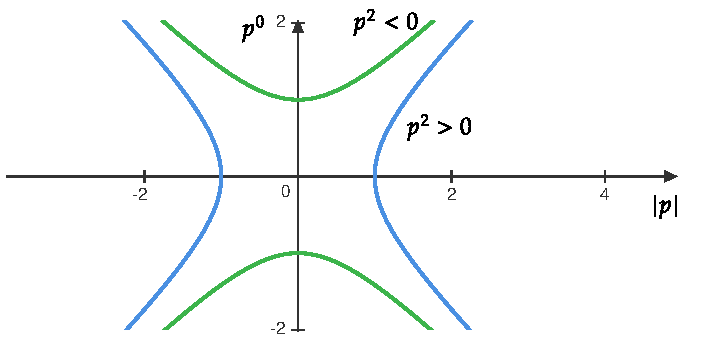
\includegraphics[scale=0.8]{p0andp.pdf}
	\label{fig:p0andp}
\end{center}

由于固有正时洛伦兹变换与单位元连通,因此只能从在图\ref{fig:p0andp}上可以看出对于$ p^{2} < 0$的曲线,两支不能通过$ \Lambda ^{\mu }{}_{\nu }$互相转换,即$ p^{0}$不能改变符号;而对于$ p^{2}  >0$的曲线,由于在$ | \boldsymbol{p}|  >0$的部分是连通的,因此$ p^{0}$的符号可以改变。



从而我们可以利用$ p^{2}$的值以及($ p^{2} \leq 0$时)的$ p^{0}$的符号来选择一个“标准动量”$ k^{\mu }$,使得
\begin{equation*}
	p^{\mu } =L^{\mu }{}_{\nu }( p) k^{\nu } ,
\end{equation*}
其中$ L^{\mu }{}_{\nu }( p)$为依赖于$ p^{\mu }$的洛伦兹变换。从而我们可以将动量为$ p$的态$ \ket{\psi ,p,\sigma }$定义为
\begin{equation*}
	\ket{\psi ,p,\sigma } \equiv N( p) U( L( p))\ket{\psi ,k,\sigma '}
\end{equation*}
其中$ N( p)$为归一化系数,稍后我们会证明$ N( p)$可以取
\begin{equation*}
	N( p) =\sqrt{\frac{k^{0}}{p^{0}}} ,
\end{equation*}
使得
\begin{equation*}
	\bra{\psi ,p',\sigma '}\ket{\psi ,p,\sigma } =\delta _{\sigma '\sigma } \delta ^{3}(\boldsymbol{p} '-\boldsymbol{p}) .
\end{equation*}
如果我们将齐次洛伦兹变换$ U( \Lambda )$作用在态$ \ket{\psi ,p,\sigma }$上,有
\begin{equation*}
	U( \Lambda )\ket{\psi ,p,\sigma } =N( p) U( \Lambda L( p))\ket{\psi ,k,\sigma } =N( p) U( L( \Lambda p)) U(L^{-1}( \Lambda p) \Lambda L( p) )\ket{\psi ,k,\sigma }
\end{equation*}
注意到变换$ L^{-1}( \Lambda p) \Lambda L( p)$先将$ k$变为$ p$,再变为$ \Lambda p$,最后再变回$ k$,因此保持$ k^{\mu }$不变。这样的保持$ k^{\mu }$不变的洛伦兹变换$ W^{\mu } \nu $构成齐次洛伦兹群的子群,被称为小群(little group)。对于这样的$ W$,我们有
\begin{equation}
	U( W)\ket{\psi ,k,\sigma } =\sum _{\sigma '} D_{\sigma '\sigma }( W)\ket{\psi ,k,\sigma '} ,
	\label{eq:litgrouprep}
\end{equation}
这样的$ D( W)$给出了小群的一个表示。那么洛伦兹变换作用在单粒子态上的效果就变成了

\begin{equation*}
	U( \Lambda )\ket{\psi ,p,\sigma } =N( p) U( L( p))\sum _{\sigma ,\sigma '} D_{\sigma ,\sigma '}( W( \Lambda ,p))\ket{\psi ,k,\sigma '} .
\end{equation*}根据$ \ket{\psi ,k,\sigma }$的定义,我们有
\begin{equation}
	\begin{aligned}
		U( \Lambda )\ket{\psi ,p,\sigma } & =\frac{N( p)}{N( \Lambda p)}\sum _{\sigma ,\sigma '} D_{\sigma ,\sigma '}( W( \Lambda ,p))\ket{\psi ,\Lambda p,\sigma '}\\
		& =\sqrt{\frac{( \Lambda p)^{0}}{p^{0}}}\sum _{\sigma ,\sigma '} D_{\sigma ,\sigma '}( W( \Lambda ,p))\ket{\psi ,\Lambda p,\sigma '} ,
		\label{eq:general_lorentz_transformation_and_litgrp}
	\end{aligned}
\end{equation}
这意味着原先的解出$C_{\sigma '\sigma }( \Lambda ,p)$在非齐次洛伦兹群不可约表示中的结构的问题现在变成了寻找小群表示$ D( W( \Lambda ,p))$的问题。在表\ref{tbl:litgrp}中,我们给出了一种标准$ k^{\mu }$的选择以及不同$ p^{2} ,p^{0}$的值给出的小群。我们的任务就是针对不同的情况,找出相应的小群表示。这被称为诱导表示法。



\begin{table}
	\centering
	\caption{不同$p^2$以及$p^0$的符号给出标准$k^{\mu}$及其对应的小群}
	\label{tbl:litgrp}
	\begin{tabular}{cllc}
		\toprule\toprule 
		& \multicolumn{1}{c}{} & \multicolumn{1}{c}{standard $ k^{\mu }$} & little group \\
		\midrule 
		(a) & $ p^{2} =-M^{2} < 0,p^{0}  >0$ & $ ( M,0,0,0)$ & $SO( 3)$ \\
		(b) & $ p^{2} =-M^{2} < 0,p^{0} < 0$ & $ ( -M,0,0,0)$ & $SO( 3)$ \\
		(c) & $ p^{2} =0,p^{0}  >0$ & $ ( \kappa ,0,0,\kappa )$ & $E( 2)$ \\
		(d) & $ p^{2} =0,p^{0} < 0$ & $ ( -\kappa ,0,0,\kappa )$ & $E( 2)$ \\
		(e) & $ p^{2} =N^{2}  >0$ & $ ( 0,0,0,N)$ & $SO( 2,1)$ \\
		(f) & $ p^{\mu } =0$ & $ ( 0,0,0,0)$ & $SO( 3,1)$ \\
		\bottomrule\bottomrule
	\end{tabular}
\end{table}



这几种情况中,只有(a),(c),(f)已知有物理解释,而(f)则是真空,因此我们只需要考虑(a),即正质量粒子的情况以及(c),即零质量粒子的情况。



下面我们考虑归一化系数的问题。首先,我们可以很自然地令$k^{\mu }$标记的态是正交的,即
\begin{equation*}
	\bra{\psi ,k',\sigma '}\ket{\psi ,k,\sigma } =\delta ^{3}(\boldsymbol{k} '-\boldsymbol{k}) \delta _{\sigma '\sigma } .
\end{equation*}
从这里我们可以看出来,小群表示$D( W)$一定是幺正的,因为
\begin{equation*}
	\begin{aligned}
		\bra{\psi ,k',\sigma '}\ket{\psi ,k,\sigma } & =\mel**{\psi ,k',\sigma '}{U^{\dagger }( \Lambda ) U( \Lambda )}{\psi ,k,\sigma }\\
		& =\sum _{\rho ,\rho '}\mel**{\psi ,k',\rho '}{D_{\rho '\sigma '}^{\dagger }( W) D_{\rho \sigma }( W)}{\psi ,k,\rho }\\
		& =\sum _{\rho ,\rho '} D_{\rho '\sigma '}^{\dagger }( W) D_{\rho \sigma }( W) \delta ^{3}(\boldsymbol{k} '-\boldsymbol{k}) \delta _{\sigma '\sigma }\\
		& =\sum _{\rho ,\rho '} D_{\rho '\sigma }^{\dagger }( W) D_{\rho \sigma }( W) \delta ^{3}(\boldsymbol{k} '-\boldsymbol{k})\stackrel{!}{=} \delta ^{3}(\boldsymbol{k} '-\boldsymbol{k}) ,
	\end{aligned}
\end{equation*}
即这意味着
\begin{equation*}
	D^{\dagger }( W) =D^{-1}( W) .
\end{equation*}
如果我们计算上述内积,可以得到:
\begin{equation*}
	\bra{\psi ,p',\sigma '}\ket{\psi ,p,\sigma } =N( p)\bra{U^{-1}( L( p)) \psi ,p',\sigma '}\ket{\psi ,k,\sigma } =N( p) N^{*}( p') D\left( W\left( L^{-1}( p) ,p'\right)\right)_{\sigma \sigma '}^{*} \delta ^{3}(\boldsymbol{k} '-\boldsymbol{k})
\end{equation*}
这里$k'\equiv L^{-1}( p) p'$。由于$k=L^{-1}( p) p$,根据$\delta $函数的性质
\begin{equation*}
	\delta ( F( x)) =\sum _{i=1}^{m}\frac{\delta ( x-a_{i})}{| F'( a_{i})| } ,F( a_{i}) =0,
\end{equation*}
我们有
\begin{equation*}
	\delta ^{3}(\boldsymbol{k} -\boldsymbol{k} ') \varpropto \delta ^{3}(\boldsymbol{p} -\boldsymbol{p} ') ,
\end{equation*}
因此随后我们需要解出比例因子。注意到对于满足$p^{2} =-M^{2} \geq 0,p^{0}  >0$的区域上,标量函数$f( p)$可以写为
\begin{equation*}
	\begin{aligned}
		\int \mathrm{d}^{4} p\delta (p^{2} +M^{2} )\theta (p^{0} )f( p) & =\int \mathrm{d}^{3}\boldsymbol{p}\mathrm{d} p^{0} \delta ((p^{0} )^{2} -\boldsymbol{p}^{2} -M^{2} )\theta (p^{0} )f(\boldsymbol{p} ,p^{0} )\\
		& =\int \mathrm{d}^{3}\boldsymbol{p}\frac{f\left(\boldsymbol{p} ,\sqrt{\boldsymbol{p}^{2} +M^{2}}\right)}{2\sqrt{\boldsymbol{p}^{2} +M^{2}}} ,
	\end{aligned}
\end{equation*}
即在$p^{2} =-M^{2}$上积分时,不变体元实际上为
\begin{equation*}
	\mathrm{d}^{3}\boldsymbol{p}\frac{f\left(\boldsymbol{p} ,\sqrt{\boldsymbol{p}^{2} +M^{2}}\right)}{\sqrt{\boldsymbol{p}^{2} +M^{2}}} .
\end{equation*}
根据$\delta $函数的定义:
\begin{equation*}
	\begin{aligned}
		F(\boldsymbol{p}) & =\int F(\boldsymbol{p} ') \delta ^{3}(\boldsymbol{p} -\boldsymbol{p} ')\mathrm{d}^{3}\boldsymbol{p} '\\
		& =\int F(\boldsymbol{p} ')\left[\sqrt{\boldsymbol{p} ^{\prime 2} +M^{2}} \delta ^{3}(\boldsymbol{p} '-\boldsymbol{p})\right]\frac{\mathrm{d}^{3}\boldsymbol{p} '}{\sqrt{\boldsymbol{p} '+M^{2}}}\\
		& =\int F(\boldsymbol{p} ')\left[ p^{0} \delta ^{3}(\boldsymbol{p} '-\boldsymbol{p})\right]\frac{\mathrm{d}^{3}\boldsymbol{p} '}{\sqrt{\boldsymbol{p} '+M^{2}}} ,
	\end{aligned}
\end{equation*}
因而我们有
\begin{equation*}
	p^{0} \delta ^{3} (\boldsymbol{p} '-\boldsymbol{p} )=k^{0} \delta ^{3} (\boldsymbol{k} '-\boldsymbol{k} ),
\end{equation*}
从而我们选择归一化因子
\begin{equation*}
	N( p) =\sqrt{\frac{k^{0}}{p^{0}}} ,
\end{equation*}
从而我们有
\begin{equation*}
	\bra{\psi ,p',\sigma '}\ket{\psi ,p,\sigma } =| N( p)| ^{2} \delta _{\sigma '\sigma }\left(\frac{p^{0}}{k^{0}}\right) \delta ^{3} (\boldsymbol{p} '-\boldsymbol{p} )=\delta _{\sigma '\sigma } \delta ^{3} (\boldsymbol{p} '-\boldsymbol{p} ).
\end{equation*}
下面我们可以考虑正质量粒子和零质量粒子给出的小群表示。

\subsubsection{正质量粒子}

正质量粒子满足的情况即$ p^{2} =-M^{2}$,其标准$ k^{\mu } =( M,0,0,0)$,保持$ k^{\mu }$不变的洛伦兹变换构成的小群为$ SO( 3)$。我们知道$ SO( 3)$的表示可以用$ D_{\sigma '\sigma }^{( j)}( R)$来分类,其中$ j$为正整数或正半整数为表示的维数。具体的表示可以用无穷小旋转$ R_{ik} =\delta _{ik} +\omega _{ik}$进行构造,其中$ \omega _{ik} =-\omega _{ik}$为无穷小量:
\begin{equation*}
	\begin{aligned}
		D_{\sigma '\sigma }^{( j)}( 1+\omega ) & =\delta _{\sigma '\sigma } +\frac{\mathrm{i}}{2} \omega _{ik} (J_{ik}^{( j)} )_{\sigma '\sigma }\\
		(J_{23}^{( j)} \pm \mathrm{i} J_{31}^{( j)} )_{\sigma ’\sigma } & =(J_{1}^{( j)} \pm \mathrm{i} J_{2}^{( j)} )=\delta _{\sigma ',\sigma \pm 1}\sqrt{( j\mp \sigma )( j\mp \sigma ) +1}\\
		(J_{12}^{( j)} )_{\sigma ’\sigma } & =(J_{3}^{( j)} )_{\sigma '\sigma } =\sigma \delta _{\sigma '\sigma } ,
	\end{aligned}
\end{equation*}
其中$ \sigma =-j,-j+1,\cdots ,j$。对于$ M >0$,自旋为$ j$的粒子,齐次洛伦兹变换作用在此单粒子态上的效果为

\begin{equation}
	U( \Lambda )\ket{\psi ,p,\sigma } =\sqrt{\frac{( \Lambda p)^{0}}{p^{0}}}\sum _{\sigma '} D_{\sigma '\sigma }^{( j)}( W( \Lambda ,p))\ket{\psi ,\Lambda p,\sigma '} ,
	\label{eq:lorentz_trans_on_single_particle_state}
\end{equation}其小群群元$ W( \Lambda ,p)$即为Wigner转动:
\begin{equation}
	W( \Lambda ,p) =L^{-1}( \Lambda p) \Lambda L( p) .
	\label{eq:little_grp_element}
\end{equation}
如果我们能证明对于任意的三维旋转$ \mathcal{R}$,$ W(\mathcal{R} ,p) =\mathcal{R}$,就是说对于一个运动的有质量粒子的态,它在旋转下的变换与非相对论量子力学中相同,那么我们可以将幼儿园学过的球谐函数,CG系数等工具直接照搬过来。

下面我们来证明这件事。首先我们需要选择一个“标准推动”$ L( p)$,使得$ k^{\mu }$变为$ p^{\mu }$。我们直接给出这样一个构造:
\begin{equation}
	\begin{aligned}
		L^{i}{}_{k}( p) & =\delta _{ik} +( \gamma -1)\hat{p}_{i}\hat{p}_{k} ,\\
		L^{i}{}_{0}( p) & =L^{0}{}_{i}( p) =\hat{p}_{i}\sqrt{\gamma ^{2} -1} ,L^{0}{}_{0}( p) =\gamma ,
		\label{eq:standard_boost}
	\end{aligned}
\end{equation}
其中
\begin{equation*}
	\hat{p}_{i} \equiv \frac{p_{i}}{| \boldsymbol{p}| } ,\gamma \equiv \frac{\sqrt{\boldsymbol{p}^{2} +M^{2}}}{M} .
\end{equation*}
我们可以验证对于$ k^{\mu } =( M,0,0,0)$,我们有:
\begin{equation*}
	\begin{aligned}
		p^{0} & =L^{0}{}_{\nu }( p) k^{\nu } =\gamma M+\hat{p}_{i}\sqrt{\gamma ^{2} -1} \cdot 0=\sqrt{\boldsymbol{p}^{2} +M^{2}} ,\\
		p^{i} & =L^{i}{}_{\nu }( p) k^{\nu } =\hat{p}^{i}\sqrt{\gamma ^{2} -1} \cdot M=\frac{p^{i}}{| \boldsymbol{p}| }\sqrt{\frac{\boldsymbol{p}^{2}}{M^{2}}} \cdot M=p^{i} ,
	\end{aligned}
\end{equation*}
即$ p^{\mu } =(\sqrt{\boldsymbol{p}^{2} +M^{2}} ,p^{i} )$,满足$ p^{\mu } p_{\mu } =-\boldsymbol{p}^{2} -M^{2} +\boldsymbol{p}^{2} =-M^{2}$。为什么$ L( p)$是一个推动?我们实际上可以发现下列关系:
\begin{equation}
	L( p) =R(\hat{\boldsymbol{p}}) B(| \boldsymbol{p}| ) R^{-1}(\hat{\boldsymbol{p}}) ,
	\label{eq:massiveLp}
\end{equation}
其中$ R(\hat{\boldsymbol{p}})$为令$ z$轴指向$ \boldsymbol{p}$方向的旋转,$ B(| \boldsymbol{p}| )$为我们熟悉的推动的标准形式:
\begin{equation*}
	B(| \boldsymbol{p}| ) =\begin{pmatrix}
		\gamma  & 0 & 0 & \sqrt{\gamma ^{2} -1}\\
		0 & 1 & 0 & 0\\
		0 & 0 & 1 & 0\\
		\sqrt{\gamma ^{2} -1} & 0 & 0 & \gamma 
	\end{pmatrix} .
\end{equation*}
这个关系是显然的,因为在令$\boldsymbol{p}$只有$z$轴分量后,$\hat{p}_{1} =\hat{p}_{2} =0,\hat{p}_{3}\hat{p}_{3} =1$,将其带入$L( p)$的表达式就可以获得$B(| \boldsymbol{p}| )$的形式。那么对于任意旋转$\mathcal{R}$,我们有
\begin{equation*}
	W(\mathcal{R} ,p)=R(\mathcal{R}\hat{\boldsymbol{p}} )B^{-1} (|\boldsymbol{p} |)R^{-1} (\mathcal{R}\hat{\boldsymbol{p}} )\mathcal{R} R(\hat{\boldsymbol{p}} )B(|\boldsymbol{p} |)R^{-1} (\hat{\boldsymbol{p}} )
\end{equation*}
但由于$R(\hat{\boldsymbol{p}})$将$z$轴转到$\hat{\boldsymbol{p}}$方向,再转到$\mathcal{R}\hat{\boldsymbol{p}}$方向,最后再转回原来的方向,因此$R^{-1} (\mathcal{R}\hat{\boldsymbol{p}} )\mathcal{R} R(\hat{\boldsymbol{p}} )$一定是朝第三轴某个方向的旋转,可以写为:
\begin{equation*}
	R^{-1} (\mathcal{R}\hat{\boldsymbol{p}} )\mathcal{R} R(\hat{\boldsymbol{p}} )=R(\theta )\equiv \begin{pmatrix}
		1 & 0 & 0 & 0\\
		0 & \cos \theta  & \sin \theta  & 0\\
		0 & -\sin \theta  & \cos \theta  & 0\\
		0 & 0 & 0 & 1
	\end{pmatrix} ,
\end{equation*}
而$R(\theta )$与$B(| \boldsymbol{p}| )$对易,因此
\begin{equation*}
	W(\mathcal{R} ,p)=R(\mathcal{R}\hat{\boldsymbol{p}} )B^{-1} (|\boldsymbol{p} |)R(\theta )B(|\boldsymbol{p} |)R^{-1} (\hat{\boldsymbol{p}} )=R(\mathcal{R}\hat{\boldsymbol{p}} )R(\theta )R^{-1} (\hat{\boldsymbol{p}} ),
\end{equation*}
即
\begin{equation*}
	W(\mathcal{R} ,p)=\mathcal{R} .
\end{equation*}
从而我们可以和非相对论量子力学一样对待有质量粒子的旋转。

\subsubsection{零质量例子}
对于无质量粒子,我们取标准的4-动量为$ k^{\mu } =( 1,0,0,1)$,小群群元$ W^{\mu }{}_{\nu }$满足$ W^{\mu }{}_{\nu } k^{\nu } =k^{\mu }$。下面我们需要解$ W$的具体形式,因此考虑$ W$作用在类时矢量$ t^{\mu } =( 1,0,0,0)$上,由于$ W$作为洛伦兹变换满足$ | W| ^{2} =1$,因此我们有
\begin{equation*}
	\begin{aligned}
		t^{\mu } t_{\mu } & =| t| ^{2} =| Wt| ^{2} =(Wt )^{\mu }( Wt)_{\mu } =-1\\
		t^{\mu } k_{\mu } & =(Wt )^{\mu }( Wk)_{\mu } =(Wt )^{\mu } k_{\mu } =-1.
	\end{aligned}
\end{equation*}
满足第二个条件的4-矢可写成
\begin{equation*}
	( Wt)^{\mu } =( 1+\zeta ,\alpha ,\beta ,\zeta ) ,
\end{equation*}
因为显然满足
\begin{equation*}
	(Wt )^{\mu } k_{\mu } =-1-\zeta +\zeta =-1.
\end{equation*}
第一个条件给出约束
\begin{equation*}
	\zeta =\frac{\alpha ^{2} +\beta ^{2}}{2} ,
\end{equation*}
因此可以知道$ W^{\mu }{}_{\nu }$作用在$ t^{\nu }$上的效果与$ S^{\mu }{}_{\nu }$作用在$ t^{\nu }$上的效果相同:
\begin{equation*}
	W^{\mu }{}_{\nu } t^{\nu } =\begin{pmatrix}
		1+\zeta \\
		\alpha \\
		\beta \\
		\zeta 
	\end{pmatrix} =\begin{pmatrix}
		1+\zeta  & \alpha  & \beta  & -\zeta \\
		\alpha  & 1 & 0 & -\alpha \\
		\beta  & 0 & 1 & -\beta \\
		\zeta  & \alpha  & \beta  & 1-\zeta 
	\end{pmatrix}\begin{pmatrix}
		1\\
		0\\
		0\\
		0
	\end{pmatrix} \equiv S^{\mu }{}_{\nu }( \alpha ,\beta ) t^{\nu }
\end{equation*}
显然,$ S^{\mu }{}_{\nu } k^{\nu } =k^{\mu }$,$ | S| =1$,且满足$ S^{\mu }{}_{\sigma } S^{\nu }{}_{\rho } \eta ^{\sigma \rho } =\eta ^{\mu \nu }$。但这不意味着$ W^{\mu }{}_{\nu } =S^{\mu }{}_{\nu }$,不过至少我们有
\begin{equation*}
	(S^{-1} W)t=t,
\end{equation*}
即保时间分量不变,因此$ S^{-1} W$为一个纯旋转;同时由于$ S^{-1} W$保$ k^{\mu } =( 1,0,0,1)$不变,因此为绕$ z$轴方向的纯旋转,可以写成
\begin{equation*}
	S^{-1}( \alpha ,\beta ) W=R( \theta ) ,R( \theta ) =\begin{pmatrix}
		1 & 0 & 0 & 0\\
		0 & \cos \theta  & \sin \theta  & 0\\
		0 & -\sin \theta  & \cos \theta  & 0\\
		0 & 0 & 0 & 1
	\end{pmatrix} .
\end{equation*}
从而我们可以写出小群群元$ W$的一般形式:
\begin{equation*}
	W( \theta ,\alpha ,\beta ) =S( \alpha ,\beta ) R( \theta ) .
\end{equation*}
下面我们看看这个群的结构:注意对子群$ \alpha =\beta =0$或者$ \theta =0$都是阿贝尔的,同时$ \theta =0$的子群为不变子群,即
\begin{equation*}
	R( \theta ) S( \alpha ,\beta ) R^{-1}( \theta ) =S( \alpha \cos \theta +\beta \sin \theta ,-\alpha \sin \theta +\beta \cos \theta ) .
\end{equation*}
因此我们可以看出这其实是$ E( 2)$的乘法规则,即平移($ \alpha ,\beta $做参数)和旋转($ \theta $做参数)构成的群。下面我们考虑$ E( 2)$的李代数:
\begin{equation*}
	W( \theta ,\alpha ,\beta )^{\mu }{}_{\nu } =\delta ^{\mu }{}_{\nu } +\omega ^{\mu }{}_{\nu } ,\omega _{\mu \nu } =\begin{pmatrix}
		0 & -\alpha  & -\beta  & 0\\
		\alpha  & 0 & \theta  & -\alpha \\
		\beta  & -\theta  & 0 & -\beta \\
		0 & \alpha  & \beta  & 0
	\end{pmatrix} .
\end{equation*}
那么相应的希尔伯特空间的算符是
\begin{equation*}
	U( W( \theta ,\alpha ,\beta )) =1+\mathrm{i} \alpha A+\mathrm{i} \beta B+\mathrm{i} \theta J_{3} ,
\end{equation*}
其中
\begin{equation*}
	\begin{aligned}
		A & =-J^{13} +J^{10} =J_{2} +K_{1} ,\\
		B & =-J^{23} +J^{20} =-J_{1} +K_{2} .
	\end{aligned}
\end{equation*}
其对易关系易得
\begin{equation*}
	\begin{aligned}
		[ J_{3} ,A] & =+\mathrm{i} B\\
		[ J_{3} ,B] & =-\mathrm{i} A\\
		[ A,B] & =0.
	\end{aligned}
\end{equation*}
由于$ A,B$对易,可以被同时对角化,因此我们有
\begin{equation*}
	\begin{aligned}
		A\ket{\psi ,a,b} & =a\ket{\psi ,a,b}\\
		B\ket{\psi ,a,b} & =b\ket{\psi ,a,b} .
	\end{aligned}
\end{equation*}
容易计算出
\begin{equation*}
	\begin{aligned}
		U[ R( \theta )] AU^{-1}[ R( \theta )] & =A\cos \theta -B\sin \theta ,\\
		U[ R( \theta )] BU^{-1}[ R( \theta )] & =A\cos \theta + B\sin \theta ,
	\end{aligned}
\end{equation*}
因而我们考虑$ A,B$作用在$ \ket{\psi ,k,\alpha ,b,\theta } \equiv U^{-1}( R( \theta ))\ket{\psi ,k,a,b}$上,有
\begin{equation*}
	\begin{aligned}
		A\ket{\psi ,a,b,\theta } & =( a\cos \theta -b\sin \theta )\ket{\psi ,k,a,b,\theta }\\
		B\ket{\psi ,a,b,\theta } & =( a\cos \theta +b\sin \theta )\ket{\psi ,k,a,b,\theta } .
	\end{aligned}
\end{equation*}
如果$ a,b$不为0,那么我们会得到一个完全连续的谱,这被称为连续自旋表示。但实验上我们并没有发现像$ \theta $这样的自由度,因此我们要求$ a=b=0$,即
\begin{equation*}
	A\ket{\psi ,k,\sigma } =B\ket{\psi ,k,\sigma } =0.
\end{equation*}
那么这些态可以通过剩下的唯一的自由度进行区分:
\begin{equation*}
	J_{3}\ket{\psi ,k,\sigma } =\sigma \ket{\psi ,k,\sigma } ,
\end{equation*}
其中$ \sigma $给出角动量在运动方向上的分量,或者称其为螺旋度。

那么随后我们就可以考察一般无质量态在洛伦兹变换下的变换性质。由于$ A,B$对易,因此任意一个小群群元可以写成
\begin{equation*}
	U( W)\ket{\psi ,k,\sigma } =\exp(\mathrm{i} \alpha A+\mathrm{i} \beta B)\exp(\mathrm{i} \theta J_{3})\ket{\psi ,k,\sigma } =\exp(\mathrm{i} \theta \sigma )\ket{\psi ,k,\sigma } .
\end{equation*}
从而,根据方程\ref{eq:litgrouprep},我们可以写出
\begin{equation*}
	D_{\sigma '\sigma }( W) =\exp(\mathrm{i} \theta \sigma ) \delta _{\sigma '\sigma } .
\end{equation*}
根据之前推出的洛伦兹变换作用在态上以小群表示作为系数的方程\ref{eq:general_lorentz_transformation_and_litgrp},我们有
\begin{equation}
	U( \Lambda )\ket{\psi ,p,\sigma } =\sqrt{\frac{( \Lambda p)^{0}}{p^{0}}}\exp(\mathrm{i} \sigma \theta ( \Lambda ,p))\ket{\psi ,\Lambda p,\sigma } ,
	\label{eq:lorentz_trans_on_massless_part}
\end{equation}
其中$ \theta ( \Lambda ,p)$定义为
\begin{equation*}
	W( \Lambda ,p) \equiv L^{-1}( \Lambda p) \Lambda L( p) \equiv S( \alpha ( \Lambda ,p) ,\beta ( \Lambda ,p)) R( \theta ( \Lambda ,p)) .
\end{equation*}
后面我们会看到,电磁理论的规范不变性来自于小群中被$ \alpha $和$ \beta $参数化的部分。目前$ \sigma $还可以取任意实数,但是某些拓扑上的原因让$ \sigma $与有质量粒子相同,只能取整数或者半整数。

我们定义
\begin{equation*}
	P_{\pm } =A\pm \mathrm{i} B,
\end{equation*}
那么根据之前的对易关系,我们可以推出
\begin{equation*}
	[ J_{3} ,P_{\pm }] =P_{\pm } ,[ P_{\pm } ,P_{\pm }] =0.
\end{equation*}
由于$ J_{3}$为$ SO( 2)$的生成元,而$ SO( 2)$的表示可以用一个整数$ m$来刻画:
\begin{equation*}
	D^{m}( R( \theta )) =\mathrm{e}^{\mathrm{i} m\theta } .
\end{equation*}
记表示$ D^{m}$的表示空间的基为$ \ket{m}$,那么群元素对态的作用自然可以表示为
\begin{equation*}
	\mathrm{e}^{\mathrm{i} \theta J_{3}}\ket{m} =D^{m} (\mathrm{e}^{\mathrm{i} \theta J_{3}} )\ket{m} =\mathrm{e}^{\mathrm{i} m\theta }\ket{m} \Rightarrow J_{3}\ket{m} =m\ket{m} ,
\end{equation*}
即$ \ket{m}$为$ J_{3}$的本征态,也因此$ m$刻画了$ SO( 2)$的不可约表示。对于$ E( 2)$,我们可以用$ SO( 2)$的不可约表示生成$ E( 2)$的忠实不可约表示。考虑$ P_{\pm }$作用在$ \ket{m}$上(此时$ \ket{m}$被看做$ E( 2)$的表示空间的一个基):
\begin{equation*}
	J_{3} (P_{\pm }\ket{m} )=([ J_{3} ,P_{\pm }] +P_{\pm } J_{3} )\ket{m} =\pm P_{\pm }\ket{m} +P_{\pm } m\ket{m} =( m\pm 1) P_{\pm }\ket{m} ,
\end{equation*}
即$ P_{\pm }\ket{m}$为$ J_{3}$的本征值为$ m\pm 1$的本征态,即$ P_{\pm }\ket{m} =\ket{m\pm 1}$。因此,当我们把$ D^{m}$当做$ E( 2)$的表示时,他们不再是单个独立的表示,而通过升降算符$ P_{\pm }$所连接,即所有可能的$ D^{m}$都被单个纳入单个的$ E( 2)$的不可约表示,并且其基为$ \{\ket{m} |m\in \mathbb{Z} \}$。

因此我们用$ J_{3}$作为小群的生成元后,其作用在单粒子态上的作用就是绕动量方向旋转,而由于在拓扑上,洛伦兹变换的底流形——非齐次洛伦兹群同构于$ \mathbb{R}_{4} \times \mathbb{R}_{3} \times S_{3} /\mathbb{Z}_{2}$,其并非单连通群,而绕动量方向角度为$ 4\pi $的旋转与单位元相同,因此$ \exp( 4\pi \mathrm{i} \sigma ) =1$,从而$ \sigma $必须是整数或者半整数。

下面我们计算给定$ \Lambda ,p$后的小群群元$ W( \Lambda ,p)$。首先我们要选一个能将$ k^{\mu } =( \kappa ,0,0,\kappa )$变为原始$ p^{\mu }$的标准洛伦兹变换:
\begin{equation*}
	L( p) =R(\hat{\boldsymbol{p}}) B(| \boldsymbol{p}| /\kappa ) ,
\end{equation*}
其中$ B( u)$为沿$ z$方向的推动:
\begin{equation*}
	B( u) =\begin{pmatrix}
		(u^{2} +1)/2u & 0 & 0 & (u^{2} -1)/2u\\
		0 & 1 & 0 & 0\\
		0 & 0 & 1 & 0\\
		(u^{2} -1)/2u & 0 & 0 & (u^{2} +1)/2u
	\end{pmatrix} ,
\end{equation*}
这里$u=\gamma \pm \sqrt{\gamma ^{2} -1} =\gamma \pm \beta $。而$ R(\hat{\boldsymbol{p}})$是使$ z$轴转向$ \hat{\boldsymbol{p}}$方向的转动,例如$ \hat{\boldsymbol{p}} =(\sin \theta \cos \phi ,\sin \theta \sin \phi ,\cos \theta )$,那么我们可以将$ R(\hat{\boldsymbol{p}})$取成绕第二轴旋转$ \theta $,从而$ ( 0,0,1)$变为$ (\sin \theta ,0,\cos \theta )$,然后再绕第三轴旋转角度$ \phi $得到$ \hat{\boldsymbol{p}}$,如图\ref{fig:standard-rotation}所示

\begin{figure}
	\centering
	
	

\tikzset{every picture/.style={line width=0.75pt}} %set default line width to 0.75pt        

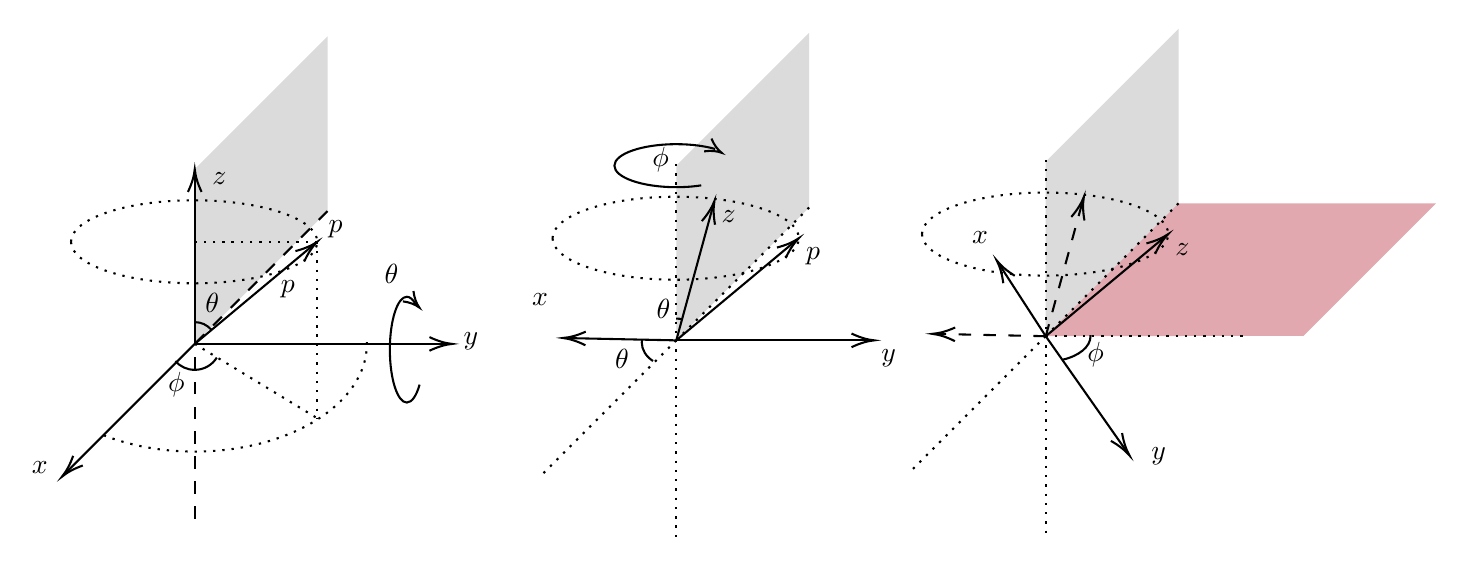
\begin{tikzpicture}[x=0.75pt,y=0.75pt,yscale=-1,xscale=1]
	%uncomment if require: \path (0,252); %set diagram left start at 0, and has height of 252
	
	%Shape: Polygon [id:ds18553688977251004] 
	\draw  [draw opacity=0][fill={rgb, 255:red, 155; green, 155; blue, 155 }  ,fill opacity=0.36 ] (376.99,5.61) -- (313,69.6) -- (313,153.76) -- (376.99,89.76) -- cycle ;
	%Straight Lines [id:da8286147690514769] 
	\draw    (313,153.76) -- (406.37,153.76) ;
	\draw [shift={(408.37,153.76)}, rotate = 180] [color={rgb, 255:red, 0; green, 0; blue, 0 }  ][line width=0.75]    (10.93,-3.29) .. controls (6.95,-1.4) and (3.31,-0.3) .. (0,0) .. controls (3.31,0.3) and (6.95,1.4) .. (10.93,3.29)   ;
	%Straight Lines [id:da9014336008611334] 
	\draw    (313,153.76) -- (330.84,88.55) ;
	\draw [shift={(331.37,86.62)}, rotate = 465.3] [color={rgb, 255:red, 0; green, 0; blue, 0 }  ][line width=0.75]    (10.93,-3.29) .. controls (6.95,-1.4) and (3.31,-0.3) .. (0,0) .. controls (3.31,0.3) and (6.95,1.4) .. (10.93,3.29)   ;
	%Straight Lines [id:da5929501825881884] 
	\draw    (313,153.76) -- (260.37,152.66) ;
	\draw [shift={(258.37,152.62)}, rotate = 361.2] [color={rgb, 255:red, 0; green, 0; blue, 0 }  ][line width=0.75]    (10.93,-3.29) .. controls (6.95,-1.4) and (3.31,-0.3) .. (0,0) .. controls (3.31,0.3) and (6.95,1.4) .. (10.93,3.29)   ;
	%Straight Lines [id:da3177504690100901] 
	\draw    (313,153.76) -- (370.47,105.84) ;
	\draw [shift={(372.01,104.56)}, rotate = 500.18] [color={rgb, 255:red, 0; green, 0; blue, 0 }  ][line width=0.75]    (10.93,-3.29) .. controls (6.95,-1.4) and (3.31,-0.3) .. (0,0) .. controls (3.31,0.3) and (6.95,1.4) .. (10.93,3.29)   ;
	%Straight Lines [id:da17393266134098084] 
	\draw  [dash pattern={on 0.84pt off 2.51pt}]  (313,68.76) -- (313,251.34) ;
	%Shape: Arc [id:dp2963276160933155] 
	\draw  [draw opacity=0] (312.87,143.26) .. controls (312.91,143.26) and (312.96,143.26) .. (313,143.26) .. controls (314.03,143.26) and (315.02,143.4) .. (315.96,143.68) -- (313,153.76) -- cycle ; \draw   (312.87,143.26) .. controls (312.91,143.26) and (312.96,143.26) .. (313,143.26) .. controls (314.03,143.26) and (315.02,143.4) .. (315.96,143.68) ;
	%Straight Lines [id:da8522591281060661] 
	\draw  [dash pattern={on 0.84pt off 2.51pt}]  (313,153.76) -- (249.01,217.75) ;
	%Straight Lines [id:da16464993164061537] 
	\draw  [dash pattern={on 0.84pt off 2.51pt}]  (376.99,89.76) -- (313,153.76) ;
	%Shape: Arc [id:dp6729156208740699] 
	\draw  [draw opacity=0] (301.8,163.72) .. controls (298.49,161.61) and (296.37,158.38) .. (296.37,154.76) .. controls (296.37,154.23) and (296.41,153.71) .. (296.5,153.19) -- (310.93,154.76) -- cycle ; \draw   (301.8,163.72) .. controls (298.49,161.61) and (296.37,158.38) .. (296.37,154.76) .. controls (296.37,154.23) and (296.41,153.71) .. (296.5,153.19) ;
	%Shape: Ellipse [id:dp4117946545762907] 
	\draw  [dash pattern={on 0.84pt off 2.51pt}] (253.37,104.56) .. controls (253.37,93.52) and (279.92,84.56) .. (312.69,84.56) .. controls (345.45,84.56) and (372.01,93.52) .. (372.01,104.56) .. controls (372.01,115.61) and (345.45,124.56) .. (312.69,124.56) .. controls (279.92,124.56) and (253.37,115.61) .. (253.37,104.56) -- cycle ;
	%Shape: Arc [id:dp49870475871297937] 
	\draw  [draw opacity=0] (325.03,79.08) .. controls (321.35,79.65) and (317.28,79.96) .. (313,79.96) .. controls (296.53,79.96) and (283.18,75.32) .. (283.18,69.6) .. controls (283.18,63.88) and (296.53,59.24) .. (313,59.24) .. controls (320.1,59.24) and (326.61,60.1) .. (331.73,61.54) -- (313,69.6) -- cycle ; \draw   (325.03,79.08) .. controls (321.35,79.65) and (317.28,79.96) .. (313,79.96) .. controls (296.53,79.96) and (283.18,75.32) .. (283.18,69.6) .. controls (283.18,63.88) and (296.53,59.24) .. (313,59.24) .. controls (320.1,59.24) and (326.61,60.1) .. (331.73,61.54) ;
	\draw   (329.94,56.53) .. controls (331.18,59.51) and (332.82,61.79) .. (334.84,63.39) .. controls (332.43,62.48) and (329.63,62.24) .. (326.43,62.7) ;
	
	%Shape: Polygon [id:ds11156348396049554] 
	\draw  [draw opacity=0][fill={rgb, 255:red, 197; green, 84; blue, 98 }  ,fill opacity=0.51 ] (679,87.76) -- (615.2,151.57) -- (491,151.76) -- (554.99,87.76) -- cycle ;
	%Straight Lines [id:da01481571122021963] 
	\draw    (491,151.76) -- (530.22,207.61) ;
	\draw [shift={(531.37,209.25)}, rotate = 234.92000000000002] [color={rgb, 255:red, 0; green, 0; blue, 0 }  ][line width=0.75]    (10.93,-3.29) .. controls (6.95,-1.4) and (3.31,-0.3) .. (0,0) .. controls (3.31,0.3) and (6.95,1.4) .. (10.93,3.29)   ;
	%Shape: Polygon [id:ds29763797832053585] 
	\draw  [draw opacity=0][fill={rgb, 255:red, 155; green, 155; blue, 155 }  ,fill opacity=0.36 ] (554.99,3.61) -- (491,67.6) -- (491,151.76) -- (554.99,87.76) -- cycle ;
	%Straight Lines [id:da6717184651887242] 
	\draw  [dash pattern={on 0.84pt off 2.51pt}]  (491,151.76) -- (586.37,151.76) ;
	%Straight Lines [id:da009520160805830402] 
	\draw    (491,151.76) -- (468.45,116.92) ;
	\draw [shift={(467.37,115.25)}, rotate = 417.09000000000003] [color={rgb, 255:red, 0; green, 0; blue, 0 }  ][line width=0.75]    (10.93,-3.29) .. controls (6.95,-1.4) and (3.31,-0.3) .. (0,0) .. controls (3.31,0.3) and (6.95,1.4) .. (10.93,3.29)   ;
	%Straight Lines [id:da3101466777730266] 
	\draw    (491,151.76) -- (548.47,103.84) ;
	\draw [shift={(550.01,102.56)}, rotate = 500.18] [color={rgb, 255:red, 0; green, 0; blue, 0 }  ][line width=0.75]    (10.93,-3.29) .. controls (6.95,-1.4) and (3.31,-0.3) .. (0,0) .. controls (3.31,0.3) and (6.95,1.4) .. (10.93,3.29)   ;
	%Straight Lines [id:da376391670348758] 
	\draw  [dash pattern={on 0.84pt off 2.51pt}]  (491,66.76) -- (491,249.34) ;
	%Straight Lines [id:da5056342698223466] 
	\draw  [dash pattern={on 0.84pt off 2.51pt}]  (491,151.76) -- (427.01,215.75) ;
	%Straight Lines [id:da39840072618958344] 
	\draw  [dash pattern={on 0.84pt off 2.51pt}]  (554.99,87.76) -- (491,151.76) ;
	%Shape: Arc [id:dp1813411465273418] 
	\draw  [draw opacity=0] (512.55,151.24) .. controls (512.57,151.41) and (512.57,151.58) .. (512.57,151.76) .. controls (512.57,156.87) and (507.03,161.25) .. (499.17,163.08) -- (491,151.76) -- cycle ; \draw   (512.55,151.24) .. controls (512.57,151.41) and (512.57,151.58) .. (512.57,151.76) .. controls (512.57,156.87) and (507.03,161.25) .. (499.17,163.08) ;
	%Straight Lines [id:da436177747427259] 
	\draw  [dash pattern={on 4.5pt off 4.5pt}]  (491,151.76) -- (508.84,86.55) ;
	\draw [shift={(509.37,84.62)}, rotate = 465.3] [color={rgb, 255:red, 0; green, 0; blue, 0 }  ][line width=0.75]    (10.93,-3.29) .. controls (6.95,-1.4) and (3.31,-0.3) .. (0,0) .. controls (3.31,0.3) and (6.95,1.4) .. (10.93,3.29)   ;
	%Shape: Ellipse [id:dp5404504293689079] 
	\draw  [dash pattern={on 0.84pt off 2.51pt}] (431.37,102.56) .. controls (431.37,91.52) and (457.92,82.56) .. (490.69,82.56) .. controls (523.45,82.56) and (550.01,91.52) .. (550.01,102.56) .. controls (550.01,113.61) and (523.45,122.56) .. (490.69,122.56) .. controls (457.92,122.56) and (431.37,113.61) .. (431.37,102.56) -- cycle ;
	%Straight Lines [id:da41467136881732425] 
	\draw  [dash pattern={on 4.5pt off 4.5pt}]  (491,151.76) -- (438.37,150.66) ;
	\draw [shift={(436.37,150.62)}, rotate = 361.2] [color={rgb, 255:red, 0; green, 0; blue, 0 }  ][line width=0.75]    (10.93,-3.29) .. controls (6.95,-1.4) and (3.31,-0.3) .. (0,0) .. controls (3.31,0.3) and (6.95,1.4) .. (10.93,3.29)   ;
	
	%Shape: Polygon [id:ds8364857098821488] 
	\draw  [draw opacity=0][fill={rgb, 255:red, 155; green, 155; blue, 155 }  ,fill opacity=0.36 ] (144.99,7.32) -- (81,71.31) -- (81,155.47) -- (144.99,91.48) -- cycle ;
	%Straight Lines [id:da8586412175269085] 
	\draw    (81,155.47) -- (203.01,155.47) ;
	\draw [shift={(205.01,155.47)}, rotate = 180] [color={rgb, 255:red, 0; green, 0; blue, 0 }  ][line width=0.75]    (10.93,-3.29) .. controls (6.95,-1.4) and (3.31,-0.3) .. (0,0) .. controls (3.31,0.3) and (6.95,1.4) .. (10.93,3.29)   ;
	%Straight Lines [id:da854032974366228] 
	\draw    (81,155.47) -- (81,73.31) ;
	\draw [shift={(81,71.31)}, rotate = 450] [color={rgb, 255:red, 0; green, 0; blue, 0 }  ][line width=0.75]    (10.93,-3.29) .. controls (6.95,-1.4) and (3.31,-0.3) .. (0,0) .. controls (3.31,0.3) and (6.95,1.4) .. (10.93,3.29)   ;
	%Straight Lines [id:da47128480383265225] 
	\draw    (81,155.47) -- (18.42,218.05) ;
	\draw [shift={(17.01,219.46)}, rotate = 315] [color={rgb, 255:red, 0; green, 0; blue, 0 }  ][line width=0.75]    (10.93,-3.29) .. controls (6.95,-1.4) and (3.31,-0.3) .. (0,0) .. controls (3.31,0.3) and (6.95,1.4) .. (10.93,3.29)   ;
	%Straight Lines [id:da613938241812592] 
	\draw    (81,155.47) -- (138.47,107.55) ;
	\draw [shift={(140.01,106.27)}, rotate = 500.18] [color={rgb, 255:red, 0; green, 0; blue, 0 }  ][line width=0.75]    (10.93,-3.29) .. controls (6.95,-1.4) and (3.31,-0.3) .. (0,0) .. controls (3.31,0.3) and (6.95,1.4) .. (10.93,3.29)   ;
	%Straight Lines [id:da8320950495713932] 
	\draw  [dash pattern={on 0.84pt off 2.51pt}]  (140.01,106.27) -- (140.01,191.27) ;
	%Straight Lines [id:da09432820232701] 
	\draw  [dash pattern={on 0.84pt off 2.51pt}]  (81,155.47) -- (140.01,191.27) ;
	%Shape: Arc [id:dp12333927429158065] 
	\draw  [draw opacity=0] (80.8,144.97) .. controls (80.86,144.97) and (80.93,144.97) .. (81,144.97) .. controls (84.19,144.97) and (87.04,146.38) .. (88.96,148.62) -- (81,155.47) -- cycle ; \draw   (80.8,144.97) .. controls (80.86,144.97) and (80.93,144.97) .. (81,144.97) .. controls (84.19,144.97) and (87.04,146.38) .. (88.96,148.62) ;
	%Shape: Arc [id:dp4722400304498686] 
	\draw  [draw opacity=0][dash pattern={on 0.84pt off 2.51pt}] (163.92,154.57) .. controls (163.93,154.87) and (163.94,155.17) .. (163.94,155.47) .. controls (163.94,184.12) and (126.8,207.34) .. (81,207.34) .. controls (64.81,207.34) and (49.71,204.44) .. (36.94,199.42) -- (81,155.47) -- cycle ; \draw  [dash pattern={on 0.84pt off 2.51pt}] (163.92,154.57) .. controls (163.93,154.87) and (163.94,155.17) .. (163.94,155.47) .. controls (163.94,184.12) and (126.8,207.34) .. (81,207.34) .. controls (64.81,207.34) and (49.71,204.44) .. (36.94,199.42) ;
	%Shape: Arc [id:dp7198902215988827] 
	\draw  [draw opacity=0] (91.62,162.07) .. controls (89.42,165.61) and (85.48,167.97) .. (81,167.97) .. controls (77.29,167.97) and (73.95,166.35) .. (71.66,163.78) -- (81,155.47) -- cycle ; \draw   (91.62,162.07) .. controls (89.42,165.61) and (85.48,167.97) .. (81,167.97) .. controls (77.29,167.97) and (73.95,166.35) .. (71.66,163.78) ;
	%Straight Lines [id:da29554111278949446] 
	\draw  [dash pattern={on 4.5pt off 4.5pt}]  (144.99,91.48) -- (81,155.47) ;
	%Straight Lines [id:da7749592314975127] 
	\draw  [dash pattern={on 4.5pt off 4.5pt}]  (81,239.63) -- (81,155.47) ;
	%Shape: Ellipse [id:dp35951516859181276] 
	\draw  [dash pattern={on 0.84pt off 2.51pt}] (21.37,106.27) .. controls (21.37,95.23) and (47.92,86.27) .. (80.69,86.27) .. controls (113.45,86.27) and (140.01,95.23) .. (140.01,106.27) .. controls (140.01,117.32) and (113.45,126.27) .. (80.69,126.27) .. controls (47.92,126.27) and (21.37,117.32) .. (21.37,106.27) -- cycle ;
	%Straight Lines [id:da8633221720382833] 
	\draw  [dash pattern={on 0.84pt off 2.51pt}]  (140.01,106.27) -- (80.69,106.27) ;
	%Shape: Arc [id:dp436825029013578] 
	\draw  [draw opacity=0] (189.32,175.09) .. controls (187.82,180.38) and (185.63,183.72) .. (183.18,183.72) .. controls (178.66,183.72) and (175,172.31) .. (175,158.23) .. controls (175,144.16) and (178.66,132.75) .. (183.18,132.75) .. controls (184.72,132.75) and (186.15,134.06) .. (187.38,136.35) -- (183.18,158.23) -- cycle ; \draw   (189.32,175.09) .. controls (187.82,180.38) and (185.63,183.72) .. (183.18,183.72) .. controls (178.66,183.72) and (175,172.31) .. (175,158.23) .. controls (175,144.16) and (178.66,132.75) .. (183.18,132.75) .. controls (184.72,132.75) and (186.15,134.06) .. (187.38,136.35) ;
	\draw   (186.37,130) .. controls (186.75,133.2) and (187.69,135.85) .. (189.2,137.95) .. controls (187.13,136.4) and (184.5,135.41) .. (181.3,134.97) ;
	
	
	% Text Node
	\draw (171,115.37) node [anchor=north west][inner sep=0.75pt]    {$\theta $};
	% Text Node
	\draw (300,59.37) node [anchor=north west][inner sep=0.75pt]    {$\phi $};
	% Text Node
	\draw (121,123.58) node [anchor=north west][inner sep=0.75pt]    {$p$};
	% Text Node
	\draw (144,94.58) node [anchor=north west][inner sep=0.75pt]    {$\boldsymbol{p}$};
	% Text Node
	\draw (84.66,129.78) node [anchor=north west][inner sep=0.75pt]    {$\theta $};
	% Text Node
	\draw (66.66,167.78) node [anchor=north west][inner sep=0.75pt]    {$\phi $};
	% Text Node
	\draw (88,71.58) node [anchor=north west][inner sep=0.75pt]    {$z$};
	% Text Node
	\draw (209,148.58) node [anchor=north west][inner sep=0.75pt]    {$y$};
	% Text Node
	\draw (1,210.58) node [anchor=north west][inner sep=0.75pt]    {$x$};
	% Text Node
	\draw (509.55,153.24) node [anchor=north west][inner sep=0.75pt]    {$\phi $};
	% Text Node
	\draw (552.01,105.56) node [anchor=north west][inner sep=0.75pt]    {$z$};
	% Text Node
	\draw (540.37,203.96) node [anchor=north west][inner sep=0.75pt]    {$y$};
	% Text Node
	\draw (454,99.87) node [anchor=north west][inner sep=0.75pt]    {$x$};
	% Text Node
	\draw (282,156.68) node [anchor=north west][inner sep=0.75pt]    {$\theta $};
	% Text Node
	\draw (302,132.68) node [anchor=north west][inner sep=0.75pt]    {$\theta $};
	% Text Node
	\draw (374.01,107.56) node [anchor=north west][inner sep=0.75pt]    {$\boldsymbol{p}$};
	% Text Node
	\draw (333.37,89.62) node [anchor=north west][inner sep=0.75pt]    {$z$};
	% Text Node
	\draw (410.37,156.76) node [anchor=north west][inner sep=0.75pt]    {$y$};
	% Text Node
	\draw (242,129.87) node [anchor=north west][inner sep=0.75pt]    {$x$};
	
	
\end{tikzpicture}
	
	\caption{将$z$轴转到$\boldsymbol{p}$方向的标准旋转}
	
	\label{fig:standard-rotation}
\end{figure}

于是我们有
\begin{equation*}
	U( R(\hat{\boldsymbol{p}})) =\exp( -\mathrm{i} \phi J_{3})\exp( -\mathrm{i} \theta J_{2}) .
\end{equation*}
当我们选择了$ L( p)$后,根据公式$ W( \Lambda ,p) \equiv L^{-1}( \Lambda p) \Lambda L( p)$我们便可直接得到$ W( \Lambda ,p)$的表达式。

注意到螺旋度是洛伦兹不变的,从而给定了$ \sigma $的无质量粒子在所有惯性系下看起来是相同的,而我们认为螺旋度不同的无质量粒子是不同种类的粒子。但实际上,螺旋度相反的粒子通过空间反演对称性相关联,而电磁力与引力都是空间反演对称的,从而我们称螺旋度为$ \pm 1$的粒子为光子,而螺旋度为$ \pm 2$的粒子为引力子。在标准模型框架下,$ \beta $衰变中发出的螺旋度为$ 1/2$的无质量粒子\footnote{对中微子质量的描述的模型超出标准模型的范畴。}并不参与引力以外的具有空间反演对称性的相互作用,因此我们称$ 1/2$螺旋度的为中微子,而$ -1/2$螺旋度的为反中微子,它们被认为是不同种粒子。我们一般认为光子和引力子为螺旋度为$ \pm 1,2$的态的线性叠加。

虽然无质量粒子的螺旋度是洛伦兹不变的,但态本身却不是,根据\ref{eq:lorentz_trans_on_massless_part},我们可以看出对于混合了正负螺旋度的光子和引力子来说,它们在一个洛伦兹变换后会变为另一个不同的态,例如4-动量为$ p$的一般光子态可以被写成
\begin{equation*}
	\ket{\psi ,p,\alpha } =\alpha _{+}\ket{\psi ,p,+1} +\alpha _{-}\ket{\psi ,p,-1} ,
\end{equation*}
其中$ | \alpha _{+}| ^{2} +| \alpha _{-}| ^{2} =1$。我们一般称这种现象为偏振。$ \alpha _{-} =\alpha _{+}^{*}$时,我们称其为线偏振,而$ \alpha _{+}$的相位可以视为偏振面与某个垂直于$ \boldsymbol{p}$的固定参考系之间的夹角,洛伦兹变换$ \Lambda $会让这个角度旋转$ \theta ( \Lambda ,p)$。注意,对于引力子的偏振,方程\ref{eq:lorentz_trans_on_massless_part}中系数$ \exp(\mathrm{i} \sigma \theta )$说明洛伦兹变换会将偏振面旋转角度$ 2\theta ( \Lambda ,p)$。

\paragraph{例1}
假设观测者$ \mathcal{O}$观测到一个$ W$玻色子(自旋为1且质量$ m\neq 0$),动量为$ \boldsymbol{p}$,动量方向为$ y$方向且自旋$ z$分量为$ \sigma $。第二个观测者$ \mathcal{O} '$相对第一个观测者以速度$ \boldsymbol{v}$沿着$ z$方向运动,那么$ \mathcal{O} '$会怎么描述$ W$的这个态?

\begin{figure}
	\centering
	
	

\tikzset{every picture/.style={line width=0.75pt}} %set default line width to 0.75pt        

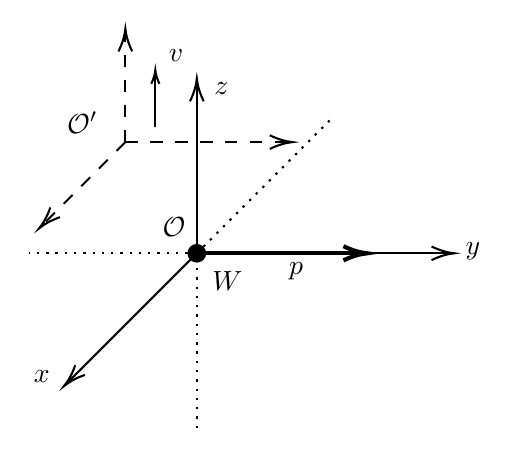
\begin{tikzpicture}[x=0.75pt,y=0.75pt,yscale=-1,xscale=1]
	%uncomment if require: \path (0,197); %set diagram left start at 0, and has height of 197
	
	%Straight Lines [id:da3320609672207786] 
	\draw  [dash pattern={on 0.84pt off 2.51pt}]  (301,109.47) -- (220,109.47) ;
	%Straight Lines [id:da0019449533056650203] 
	\draw    (301,109.47) -- (423.01,109.47) ;
	\draw [shift={(425.01,109.47)}, rotate = 180] [color={rgb, 255:red, 0; green, 0; blue, 0 }  ][line width=0.75]    (10.93,-3.29) .. controls (6.95,-1.4) and (3.31,-0.3) .. (0,0) .. controls (3.31,0.3) and (6.95,1.4) .. (10.93,3.29)   ;
	%Straight Lines [id:da35965824565982163] 
	\draw    (301,109.47) -- (301,27.31) ;
	\draw [shift={(301,25.31)}, rotate = 450] [color={rgb, 255:red, 0; green, 0; blue, 0 }  ][line width=0.75]    (10.93,-3.29) .. controls (6.95,-1.4) and (3.31,-0.3) .. (0,0) .. controls (3.31,0.3) and (6.95,1.4) .. (10.93,3.29)   ;
	%Straight Lines [id:da24691145277823567] 
	\draw    (301,109.47) -- (238.42,172.05) ;
	\draw [shift={(237.01,173.46)}, rotate = 315] [color={rgb, 255:red, 0; green, 0; blue, 0 }  ][line width=0.75]    (10.93,-3.29) .. controls (6.95,-1.4) and (3.31,-0.3) .. (0,0) .. controls (3.31,0.3) and (6.95,1.4) .. (10.93,3.29)   ;
	%Straight Lines [id:da7876238424914852] 
	\draw [line width=1.5]    (301,109.47) -- (380,109.47) ;
	\draw [shift={(383,109.47)}, rotate = 180] [color={rgb, 255:red, 0; green, 0; blue, 0 }  ][line width=1.5]    (11.37,-3.42) .. controls (7.23,-1.45) and (3.44,-0.31) .. (0,0) .. controls (3.44,0.31) and (7.23,1.45) .. (11.37,3.42)   ;
	\draw [shift={(301,109.47)}, rotate = 0] [color={rgb, 255:red, 0; green, 0; blue, 0 }  ][fill={rgb, 255:red, 0; green, 0; blue, 0 }  ][line width=1.5]      (0, 0) circle [x radius= 3.48, y radius= 3.48]   ;
	%Straight Lines [id:da5550885761878284] 
	\draw  [dash pattern={on 0.84pt off 2.51pt}]  (364.99,45.48) -- (301,109.47) ;
	%Straight Lines [id:da6613513151925012] 
	\draw  [dash pattern={on 0.84pt off 2.51pt}]  (301,193.63) -- (301,109.47) ;
	%Straight Lines [id:da21238637764144053] 
	\draw  [dash pattern={on 4.5pt off 4.5pt}]  (266.56,55.91) -- (345.07,55.91) ;
	\draw [shift={(347.07,55.91)}, rotate = 180] [color={rgb, 255:red, 0; green, 0; blue, 0 }  ][line width=0.75]    (10.93,-3.29) .. controls (6.95,-1.4) and (3.31,-0.3) .. (0,0) .. controls (3.31,0.3) and (6.95,1.4) .. (10.93,3.29)   ;
	%Straight Lines [id:da1528335475321898] 
	\draw  [dash pattern={on 4.5pt off 4.5pt}]  (266.56,55.91) -- (266.56,3.27) ;
	\draw [shift={(266.56,1.27)}, rotate = 450] [color={rgb, 255:red, 0; green, 0; blue, 0 }  ][line width=0.75]    (10.93,-3.29) .. controls (6.95,-1.4) and (3.31,-0.3) .. (0,0) .. controls (3.31,0.3) and (6.95,1.4) .. (10.93,3.29)   ;
	%Straight Lines [id:da1861354405272635] 
	\draw  [dash pattern={on 4.5pt off 4.5pt}]  (266.56,55.91) -- (226.42,96.05) ;
	\draw [shift={(225.01,97.46)}, rotate = 315] [color={rgb, 255:red, 0; green, 0; blue, 0 }  ][line width=0.75]    (10.93,-3.29) .. controls (6.95,-1.4) and (3.31,-0.3) .. (0,0) .. controls (3.31,0.3) and (6.95,1.4) .. (10.93,3.29)   ;
	%Straight Lines [id:da4199529155239894] 
	\draw [line width=0.75]    (281,48.47) -- (281,23.27) ;
	\draw [shift={(281,21.27)}, rotate = 450] [color={rgb, 255:red, 0; green, 0; blue, 0 }  ][line width=0.75]    (6.56,-1.97) .. controls (4.17,-0.84) and (1.99,-0.18) .. (0,0) .. controls (1.99,0.18) and (4.17,0.84) .. (6.56,1.97)   ;
	
	% Text Node
	\draw (221,164.58) node [anchor=north west][inner sep=0.75pt]    {$x$};
	% Text Node
	\draw (429,102.58) node [anchor=north west][inner sep=0.75pt]    {$y$};
	% Text Node
	\draw (308,25.58) node [anchor=north west][inner sep=0.75pt]    {$z$};
	% Text Node
	\draw (344,112.47) node [anchor=north west][inner sep=0.75pt]    {$\boldsymbol{p}$};
	% Text Node
	\draw (283,91) node [anchor=north west][inner sep=0.75pt]    {$\mathcal{O}$};
	% Text Node
	\draw (237,40) node [anchor=north west][inner sep=0.75pt]    {$\mathcal{O} '$};
	% Text Node
	\draw (286,10) node [anchor=north west][inner sep=0.75pt]    {$\boldsymbol{v}$};
	% Text Node
	\draw (307,117) node [anchor=north west][inner sep=0.75pt]    {$W$};
	
	
\end{tikzpicture}
	
	\caption{以$\mathcal{O}$为静止系观察动量为$y$方向的粒子。}
\end{figure}

在$ \mathcal{O}$系下,我们标记这个本征态为$ \ket{\psi ,p,\sigma }$,其中$ p=(p^{0} ,0,\rho ,0),p^{0} =\sqrt{\rho ^{2} +m^{2}} ,\rho \equiv | \boldsymbol{p}| $。我们选择标准$ k^{\mu } =( m,0,0,0,0)$,那么根据之前推出的变换规则(3)
\begin{equation*}
	U( \Lambda )\ket{\psi ,p,\sigma } =\sqrt{\frac{( \Lambda p)^{0}}{p^{0}}}\sum _{\sigma '} D_{\sigma '\sigma }^{( j)}( W( \Lambda ,p))\ket{\psi ,\Lambda p,\sigma '} ,
\end{equation*}
便可计算。首先我们需要知道小群群元(4):
\begin{equation*}
	W( \Lambda ,p) =L^{-1}( \Lambda p) \Lambda L( p) ,
\end{equation*}
这里我们的洛伦兹变换为
\begin{equation*}
	\Lambda ( v)^{\mu }{}_{\nu } =\begin{pmatrix}
		\gamma  & 0 & 0 & \sqrt{\gamma ^{2} -1}\\
		0 & 1 & 0 & 0\\
		0 & 0 & 1 & 0\\
		\sqrt{\gamma ^{2} -1} & 0 & 0 & \gamma 
	\end{pmatrix} ,\gamma =\frac{1}{\sqrt{1-v^{2}}} .
\end{equation*}
而我们选取的将$k^{\mu }{}_{\nu }$变回$p^{\mu }{}_{\nu }$的洛伦兹变换为:
\begin{equation*}
	L( p)^{\mu }{}_{\nu } =R(\hat{\boldsymbol{p}})\begin{pmatrix}
		\gamma ' & 0 & 0 & \sqrt{\gamma ^{\prime 2} -1}\\
		0 & 1 & 0 & 0\\
		0 & 0 & 1 & 0\\
		\sqrt{\gamma ^{\prime 2} -1} & 0 & 0 & \gamma '
	\end{pmatrix} R^{-1}(\hat{\boldsymbol{p}}) ,\gamma \equiv \frac{\sqrt{\boldsymbol{p}^{2} +m^{2}}}{m} .
\end{equation*}
注意这里,$\gamma $给出$\mathcal{O}$和$\mathcal{O} '$之间的洛伦兹变换,而$\gamma '$则是我们选择的“标准推动”的参数,依赖于四矢量$p$。那么我们可以计算出$W( \Lambda ,p) =L^{-1}( \Lambda p) \Lambda L( p)$的具体值为
\begin{equation}
	W( \Lambda ,p)^{\mu }{}_{\nu } =\left(\begin{matrix}
		1 & 0 & 0 & 0\\
		0 & 1 & 0 & 0\\
		0 & 0 & \cos \theta  & -\sin \theta \\
		0 & 0 & \sin \theta  & \cos \theta 
	\end{matrix}\right) =\mathscr{R}( \theta ) ,
\end{equation}
其中
\begin{equation*}
	\cos \theta =\frac{\gamma \left( \gamma m\sqrt{m^{2} +\rho ^{2}} +\rho ^{2}\right) -m\sqrt{m^{2} +\rho ^{2}}}{\gamma ^{2} \rho ^{2} +\left( \gamma ^{2} -1\right) m^{2}} ,\sin \theta =\frac{\rho \left( -\sqrt{\gamma ^{2} -1} m+\gamma \sqrt{\left( \gamma ^{2} -1\right)\left( m^{2} +\rho ^{2}\right)}\right)}{\gamma ^{2} \rho ^{2} +\left( \gamma ^{2} -1\right) m^{2}} .
\end{equation*}
注意这里在计算时,$L^{-1}( \Lambda p)$中需要计算$R(\mathbf{\Lambda }\boldsymbol{p})$,而非简单的$R(\boldsymbol{p})$。我们可以发现,$W$确实是小群$SO( 3)$的群元:
\begin{equation*}
	W^{\mu }{}_{\nu } k^{\nu } =k^{\mu } ,W^{\mu }{}_{\nu } W^{\nu }{}_{\rho } =\delta ^{\mu }{}_{\rho } .
\end{equation*}
那么由于$W$玻色子的自旋$j=1$,我们需要求出$D^{1}( W)$,即Wigner旋转。考虑对$SO( 3)$的一个元素$R$做$z-y-z$分解,即将一个旋转写成
\begin{equation*}
	R( \alpha ,\beta ,\gamma ) =R_{z}( \alpha ) R_{y}( \beta ) R_{z}( \gamma ) =\mathrm{e}^{-\mathrm{i} \alpha J_{3}}\mathrm{e}^{-\mathrm{i} \beta J_{2}}\mathrm{e}^{-\mathrm{i} \gamma J_{3}} ,
\end{equation*}
其中$\alpha ,\beta ,\gamma $为该旋转的欧拉角。那么表示$D^{( 1)}( R)$为:
\begin{equation*}
	D^{( 1)} (\alpha ,\beta ,\gamma )=\left(\begin{matrix}
		\mathrm{e}^{\mathrm{i} (\alpha +\gamma )}\cos^{2}\frac{\beta }{2} & -\frac{\mathrm{e}^{\mathrm{i} \alpha }\sin \beta }{\sqrt{2}} & \mathrm{e}^{\mathrm{i} (\alpha -\gamma )}\sin^{2}\frac{\beta }{2}\\
		\frac{\mathrm{e}^{\mathrm{i} \gamma }\sin \beta }{\sqrt{2}} & \cos \beta  & -\frac{\mathrm{e}^{-\mathrm{i} \gamma }\sin \beta }{\sqrt{2}}\\
		\mathrm{e}^{-\mathrm{i} (\alpha -\gamma )}\sin^{2}\frac{\beta }{2} & \frac{\mathrm{e}^{-\mathrm{i} \alpha }\sin \beta }{\sqrt{2}} & \mathrm{e}^{-\mathrm{i} (\alpha +\gamma )}\cos^{2}\frac{\beta }{2}
	\end{matrix}\right)\text{. }
\end{equation*}
对于$W( \Lambda ,p)$,这是一个绕$x$轴的旋转,那么我们只需先将绕$z$轴旋转使得$x$轴与原来的$y$轴重合,再沿着$y$轴旋转原来的角度,最后转回去即可,那么我们得到
\begin{equation*}
	\mathscr{R}( \alpha ,\beta ,\gamma ) =R_{z}\left( -\frac{\pi }{2}\right) R_{y}( \theta ) R_{z}\left(\frac{\pi }{2}\right) =\begin{pmatrix}
		0 & 1 & 0\\
		-1 & 0 & 0\\
		0 & 0 & 1
	\end{pmatrix}\begin{pmatrix}
		\cos \theta  & 0 & \sin \theta \\
		0 & 1 & 0\\
		-\sin \theta  & 0 & \cos \theta 
	\end{pmatrix}\begin{pmatrix}
		0 & -1 & 0\\
		1 & 0 & 0\\
		0 & 0 & 1
	\end{pmatrix} .
\end{equation*}
于是$D^{( 1)}( W)$就为
\begin{equation*}
	D^{( 1)} (W)=\left(\begin{matrix}
		\cos^{2}\frac{\theta }{2} & \frac{\mathrm{i}\sin \theta }{\sqrt{2}} & -\sin^{2}\frac{\theta }{2}\\
		\frac{\mathrm{i}\sin \theta }{\sqrt{2}} & \cos \theta  & \frac{\mathrm{i}\sin \theta }{\sqrt{2}}\\
		-\sin^{2}\frac{\theta }{2} & \frac{\mathrm{i}\sin \theta }{\sqrt{2}} & \cos^{2}\frac{\theta }{2}
	\end{matrix}\right) .
\end{equation*}
那么,作用了该洛伦兹变换后,该单粒子态变为
\begin{equation*}
	U( \Lambda )\ket{\psi ,p,\sigma } =\sqrt{\frac{( \Lambda p)^{0}}{p^{0}}}\sum _{\sigma '} D_{\sigma '\sigma }^{( j)}( W( \Lambda ,p))\ket{\psi ,\Lambda p,\sigma '} =\sqrt{\gamma }\sum _{\sigma '\in \{-1,0,1\}} D_{\sigma '\sigma }^{( 1)}( W)\ket{\psi ,\Lambda p,\sigma '} .
\end{equation*}
例如,如果$\sigma =-1$,那么我们有
\begin{equation*}
	\begin{aligned}
		U( \Lambda )\ket{\psi ,p,-1} & =\sqrt{\gamma }\left( D_{-1,-1}^{( 1)}( W)\ket{\psi ,\Lambda p,-1} +D_{0,-1}^{( 1)}( W)\ket{\psi ,\Lambda p,0} +D_{1,-1}^{( 1)}( W)\ket{\psi ,\Lambda p,1}\right)\\
		& =\sqrt{\gamma }\left(\cos^{2}\frac{\theta }{2}\ket{\psi ,\Lambda p,-1} +\frac{\mathrm{i}\sin \theta }{\sqrt{2}}\ket{\psi ,\Lambda p,-1} -\sin^{2}\frac{\theta }{2}\ket{\psi ,\Lambda p,1}\right) .
	\end{aligned}
\end{equation*}

\paragraph{例2}
假设观测者$ \mathcal{O}$观测到一个光子,动量为$ \boldsymbol{p}$,动量方向为$ y$方向且极化矢量在$z$方向。第二个观测者$ \mathcal{O} '$相对第一个观测者以速度$ \boldsymbol{v}$沿着$ z$方向运动,那么$ \mathcal{O} '$会怎么描述这个光子?

首先我们需要将该光子的态写出来:
\begin{equation*}
	\ket{\psi ,p,\alpha } =\alpha _{+}\ket{\psi ,p,1} +\alpha _{-}\ket{\psi ,p,-1} ,
\end{equation*}
随后根据之前给出的式\ref{eq:lorentz_trans_on_massless_part}
\begin{equation*}
	U( \Lambda )\ket{\psi ,p,\sigma } =\sqrt{\frac{( \Lambda p)^{0}}{p^{0}}}\exp(\mathrm{i} \sigma \theta ( \Lambda ,p))\ket{\psi ,\Lambda p,\sigma }
\end{equation*}
计算即可。与有质量态的情况相似,区别在于我们选择标准4动量为$k^{\mu } =( 1,0,0,1)$。我们首先计算小群群元$W( \Lambda ,p)$。取$L( p) =R(\hat{\boldsymbol{p}}) B(| \boldsymbol{p}| )$,我们有
\begin{equation*}
	W( \Lambda ,p) =\left(\begin{matrix}
		1-\frac{1-\gamma ^{2}}{2\rho ^{2} \gamma ^{2}} & -\frac{\sqrt{\gamma ^{2} -1}}{\gamma \rho } & 0 & -\frac{\gamma ^{2} -1}{2\gamma ^{2} \rho ^{2}}\\
		-\frac{\sqrt{\gamma ^{2} -1}}{\gamma \rho } & 1 & 0 & \frac{\sqrt{\gamma ^{2} -1}}{\gamma \rho }\\
		0 & 0 & 1 & 0\\
		\frac{\gamma ^{2} -1}{2\gamma ^{2} \rho ^{2}} & -\frac{\sqrt{\gamma ^{2} -1}}{\gamma \rho } & 0 & \frac{1-\gamma ^{2}}{2\rho ^{2} \gamma ^{2}} +1
	\end{matrix}\right) =S( \alpha ,\beta ) R( \theta ) .
\end{equation*}
下面我们需要将$W$分解,求出参数$\theta $。由于
\begin{equation*}
	S( \alpha ,\beta ) R( \theta ) =\left(\begin{array}{ c c c c }
		\zeta +1 & \alpha \cos \theta -\beta \sin \theta  & \alpha \sin \theta +\beta \cos \theta  & -\zeta \\
		\alpha  & \cos \theta  & \sin \theta  & -\alpha \\
		\beta  & -\sin \theta  & \cos \theta  & -\beta \\
		\zeta  & \alpha \cos \theta -\beta \sin \theta  & \alpha \sin \theta +\beta \cos \theta  & 1-\zeta 
	\end{array}\right) ,
\end{equation*}
对比系数可得
\begin{equation*}
	\zeta =\frac{\gamma ^{2} -1}{2\gamma ^{2} \rho ^{2}} ,\alpha =-\frac{\sqrt{\gamma ^{2} -1}}{\gamma \rho } ,\beta =0,\theta =0.
\end{equation*}
从而作用了该洛伦兹变换后,该单粒子态变为
\begin{equation*}
	U( \Lambda )\ket{\psi ,p,\alpha } =\sqrt{\gamma }\left( \alpha _{+}\ket{\psi ,p,1} +\alpha _{-}\ket{\psi ,p,-1}\right) .
\end{equation*}

\subsubsection{时间反演与空间反演}
我们已经知道,任何齐次洛伦兹变换都可以由固有正时洛伦兹变换($ \det \Lambda =1,\Lambda ^{0}{}_{0} \geq 0$)以及时间反演$ \mathscr{T}$和空间反演$ \mathscr{P}$生成,这里$ \mathscr{T}$和$ \mathscr{P}$为
\begin{equation*}
	\mathscr{P}^{\mu }{}_{\nu } =\begin{pmatrix}
		1 &  &  & \\
		& -1 &  & \\
		&  & -1 & \\
		&  &  & -1
	\end{pmatrix} ,\mathscr{T}^{\mu }{}_{\nu } =\begin{pmatrix}
		-1 &  &  & \\
		& 1 &  & \\
		&  & 1 & \\
		&  &  & 1
	\end{pmatrix} .
\end{equation*}
曾经人们相信对于包含了$ \mathscr{P} ,\mathscr{T}$的$ \Lambda $,庞加莱群的乘积规则
\begin{equation*}
	U( \Lambda _{1} ,a_{1}) U( \Lambda _{2} ,a_{2}) =U( \Lambda _{1} \Lambda _{2} ,\Lambda _{2} a_{2} +a_{1})
\end{equation*}
是不证自明的,同时人们也相信对应于$ \mathscr{P} ,\mathscr{T}$的算符$ \mathsf{P} \equiv U(\mathscr{P} ,0) ,\mathsf{T} \equiv U(\mathscr{T} ,0)$,以及任何固有正时洛伦兹变换$ \Lambda ^{\mu }{}_{\nu }$和平移$ a^{\mu }$,都有
\begin{equation}
	\begin{aligned}
		\mathsf{P} U( \Lambda ,a)\mathsf{P}^{-1} & =U(\mathscr{P} \Lambda \mathscr{P}^{-1} ,\mathscr{P} a),\\
		\mathsf{T} U( \Lambda ,a)\mathsf{T}^{-1} & =U(\mathscr{T} \Lambda \mathscr{T}^{-1} ,\mathscr{T} a).
		\label{eq:cpconservation}
	\end{aligned}
\end{equation}
这就是我们通常所说的“宇称守恒”的含义。但后来人们才意识到,这些仅在弱相互作用可以被忽略的近似下,对于$ \mathsf{P} ,\mathsf{T}$才是近似正确的。在后文中,我们先假设满足方程\ref{eq:cpconservation}的算符$ \mathsf{P} ,\mathsf{T}$真的存在。

下面考虑无穷小洛伦兹变换,即
\begin{equation*}
	\Lambda ^{\mu }{}_{\nu } =\delta ^{\mu }{}_{\nu } +\omega ^{\mu }{}_{\nu } ,a^{\mu } =\epsilon ^{\mu } ,
\end{equation*}
那么
\begin{equation*}
	\begin{aligned}
		\Lambda ^{\prime \mu }_{\nu } =\mathscr{P}^{\mu }{}_{\rho }\mathscr{(\delta ^{\rho }{}_{\sigma } +\omega ^{\rho }{}_{\sigma } )P}^{\sigma }{}_{\nu } & =\delta ^{\mu }{}_{\nu } +\mathscr{P}^{\mu }{}_{\rho }\mathscr{\omega ^{\rho }{}_{\sigma } P}^{\sigma }{}_{\nu } ,\\
		a^{\prime \mu } & =\mathscr{P}^{\mu }{}_{\nu } \epsilon ^{\nu } .
	\end{aligned}
\end{equation*}
带入其表示
\begin{equation*}
	U( 1+\omega ,\epsilon ) =1+\frac{\mathrm{i}}{2} \omega _{\rho \sigma } J^{\rho \sigma } -\mathrm{i} \epsilon _{\rho } P^{\rho } ,
\end{equation*}
我们可以得到$\mathsf{P}$和$\mathsf{T}$的变换性质:
\begin{equation*}
	\begin{aligned}
		\mathsf{P} (1+\frac{\mathrm{i}}{2} \omega _{\rho \sigma } J^{\rho \sigma } -\mathrm{i} \epsilon _{\rho } P^{\rho } )\mathsf{P}^{-1} & =1+\mathsf{P}\frac{\mathrm{i}}{2} \omega _{\rho \sigma } J^{\rho \sigma }\mathsf{P}^{-1} -\mathbb{P}\mathrm{i} \epsilon _{\rho } P^{\rho }\mathsf{P}^{-1}\\
		& \stackrel{!}{=} 1+\frac{\mathrm{i}}{2}\mathscr{P}_{\rho \alpha }\mathscr{\omega ^{\alpha }{}_{\beta } P}^{\beta }{}_{\sigma } J^{\rho \sigma } -\mathrm{i}\mathscr{P}_{\rho \sigma } \epsilon ^{\sigma } P^{\rho }
	\end{aligned}
\end{equation*}
令$\omega _{\rho \sigma } ,\epsilon _{\rho }$的系数相等,我们有
\begin{equation*}
	\mathsf{P}\mathrm{i} J^{\rho \sigma }\mathsf{P}^{-1} =\mathrm{i}\mathscr{P}{_{\mu }}\mathscr{^{\rho } P}{_{\nu }}^{\sigma } J^{\mu } ,\mathsf{P}\mathrm{i} P^{\rho }\mathsf{P}^{-1} =\mathrm{i}\mathscr{P}{_{\mu }}^{\rho } P^{\mu } .
\end{equation*}
对于$\mathsf{T}$,我们可以同样计算得到
\begin{equation*}
	\mathsf{T}\mathrm{i} J^{\rho \sigma }\mathsf{T}^{-1} =\mathrm{i}\mathscr{T}{_{\mu }}\mathscr{^{\rho } T}{_{\nu }}^{\sigma } J^{\mu } ,\mathsf{T}\mathrm{i} P^{\rho }\mathsf{T}^{-1} =\mathrm{i}\mathscr{T}{_{\mu }}^{\rho } P^{\mu } .
\end{equation*}
注意,这里我们没有消掉两边的$\mathrm{i}$是因为这时我们还没决定$\mathsf{P} ,\mathsf{T}$是线性还是反线性(即是否与$\mathrm{i}$反对易)的。但如果我们令$\rho =0$,便可以得到
\begin{equation*}
	\mathsf{P}\mathrm{i} H\mathsf{P}^{-1} =\mathrm{i} H,
\end{equation*}
其中$H=P^{0}$为能量。如果$\mathsf{P}$反线性且反幺正,那么它与$\mathrm{i}$反对易,从而有$\mathsf{P} H\mathsf{P}^{-1} =-H$,但这意味着对于一个能量为$E >0$的态$\ket{\psi }$,我们有
\begin{equation*}
	H\mathsf{P}^{-1}\ket{\psi } =-\mathsf{P}^{-1} H\ket{\psi } =-\mathsf{P}^{-1} E\ket{\psi } =-E\mathsf{P}^{-1}\ket{\psi } ,
\end{equation*}
即存在一个能量为$-E$的态$\mathsf{P}^{-1}\ket{\psi }$,但由于不可能存在比真空能量还低的态,因此$\mathsf{P}$必须是线性且幺正的,并且与$H$对易。

同理,对于$\mathsf{T}$,我们同样有
\begin{equation*}
	\mathsf{T}\mathrm{i} H\mathsf{T}^{-1} =-\mathrm{i} H,
\end{equation*}
若$\mathsf{T}$是幺正且线性的,我们也可以得出同样的矛盾,因此$\mathsf{T}$必须是反线性且反幺正的。从而我们有
\begin{equation*}
	\mathsf{P} H\mathsf{P}^{-1} =\mathsf{T} H\mathsf{T}^{-1} =H
\end{equation*}
在加上其他几个分量:
\begin{equation*}
	\begin{array}{ l c }
		\mathsf{P}\boldsymbol{J}\mathsf{P}^{-1} =+\boldsymbol{J} , & \mathsf{T}\boldsymbol{J}\mathsf{T}^{-1} =-\boldsymbol{J} ,\\
		\mathsf{P}\boldsymbol{K}\mathsf{P}^{-1} =-\boldsymbol{K} , & \mathsf{T}\boldsymbol{K}\mathsf{T}^{-1} =+\boldsymbol{K} ,\\
		\mathsf{P}\boldsymbol{P}\mathsf{P}^{-1} =-\mathbf{P} , & \mathsf{T}\boldsymbol{P}\mathsf{T}^{-1} =-\boldsymbol{P} .
	\end{array}
\end{equation*}
记得其中
\begin{equation*}
	\boldsymbol{J} =\{J^{23} ,J^{31} ,J^{12} \},\boldsymbol{K} =\{J^{01} ,J^{02} ,J^{03} \},\boldsymbol{P} =\{P^{3} ,P^{2} ,P^{1} \}.
\end{equation*}
我们可以轻松证明上述关系和庞加莱群的对易关系是相容的,例如对于
\begin{equation*}
	[ J_{i} ,J_{j}] =\mathrm{i} \epsilon _{ijk} J_{k} ,
\end{equation*}
我们有
\begin{equation*}
	\begin{aligned}
		[ J_{i} ,J_{j}] =[\mathsf{P} J_{i}\mathsf{P}^{-1} ,\mathsf{P} J_{j}\mathsf{P}^{-1} ] & =\mathsf{P} J_{i}\mathsf{P}^{-1}\mathsf{P} J_{j}\mathsf{P}^{-1} -\mathsf{P} J_{j}\mathsf{P}^{-1}\mathsf{P} J_{i}\mathsf{P}^{-1}\\
		& =\mathsf{P} [J_{i} ,J_{j} ]\mathsf{P}^{-1}\\
		& =\mathsf{P}\mathrm{i} \epsilon _{ijk} J_{k}\mathsf{P}^{-1}\\
		& =\mathrm{i} \epsilon _{ijk}\mathsf{P} J_{k}\mathsf{P}^{-1} =\mathrm{i} \epsilon _{ijk} J_{k} .
	\end{aligned}
\end{equation*}
下面我们考虑$\mathsf{T} ,\mathsf{P}$对单粒子态的作用。

\paragraph{正质量态,空间反演}
我们将单粒子态$\ket{\psi ,k,\sigma }$定义为$\boldsymbol{P} ,H,J_{3}$的本征矢,本征值分别为$0,M,\sigma $。根据我们得到的对易关系:
\begin{equation*}
	\mathsf{P} J_{3}\ket{\psi ,k,\sigma } =\mathsf{P} \sigma \ket{\psi ,k,\sigma } =\sigma \mathsf{P}\ket{\psi ,k,\sigma } =J_{3} P\ket{\psi ,k,\sigma } ,
\end{equation*}
因此我们知道$\mathsf{P}\ket{\psi ,k,\sigma }$对$\boldsymbol{P} ,H,J_{3}$的本征值同样为$0,M,\sigma $,且与本来的态只差一个相位
\begin{equation*}
	\mathsf{P}\ket{\psi ,k,\sigma } =\eta _{\sigma }\ket{\psi ,k,\sigma } .
\end{equation*}
实际上,$\eta _{\sigma }$独立于$\sigma $,因为由
\begin{equation*}
	J_{1} \pm \mathrm{i} J_{2}\ket{\psi ,k,\sigma } =\sqrt{( j\mp \sigma )( j\pm \sigma +1)}\ket{\psi ,k,\sigma \pm 1} ,
\end{equation*}
两边作用$\mathsf{P}$,我们有
\begin{equation*}
	\eta _{\sigma } =\eta _{\sigma \pm 1} .
\end{equation*}
从而
\begin{equation*}
	\mathsf{P}\ket{\psi ,k,\sigma } =\eta \ket{\psi ,k,\sigma } ,
\end{equation*}
我们称相位$\eta $为内禀宇称,因为它仅依赖于$\mathsf{P}$所作用的粒子种类。对于一般的动量$p$态,我们有
\begin{equation*}
	\ket{\psi ,p,\sigma } =\sqrt{\frac{M}{p^{0}}} U( L( p))\ket{\psi ,k,\sigma } ,
\end{equation*}
其中对于$L( p)$,我们选择式\ref{eq:standard_boost}所给出的标准推动。注意到(写成矩阵形式则是显然的):
\begin{equation*}
	\mathscr{P} L( p)\mathscr{P}^{-1} =L(\mathscr{P} p) ,\mathscr{P} p=\left(\sqrt{\boldsymbol{p}^{2} +M^{2}} ,-\boldsymbol{p}\right) ,
\end{equation*}
我们有
\begin{equation*}
	\mathsf{P}\ket{\psi ,p,\sigma } =\sqrt{\frac{M}{p^{0}}}\mathsf{P} U( L( p))\ket{\psi ,k,\sigma } =\sqrt{\frac{M}{p^{0}}}\mathsf{P} U( L( p))\mathsf{P}^{-1}\mathsf{P}\ket{\psi ,k,\sigma } =\sqrt{\frac{M}{p^{0}}} U( L(\mathscr{P} p)) \eta \ket{\psi ,k,\sigma } ,
\end{equation*}
即
\begin{equation*}
	\mathsf{P}\ket{\psi ,p,\sigma } =\eta \ket{\psi ,\mathscr{P} p,\sigma } .
\end{equation*}

\paragraph{正质量态,时间反演}
与之前相同,我们可以直接看出$\mathsf{T}$作用在$\ket{\psi ,k,\sigma }$上的效果是
\begin{equation*}
	\boldsymbol{P} (\mathsf{T}\ket{\psi ,k,\sigma } )=0,H(\mathsf{T}\ket{\psi ,k,\sigma } )=M(\mathsf{T}\ket{\psi ,k,\sigma } ),J_{3} (\mathsf{T}\ket{\psi ,k,\sigma } )=-\sigma (\mathsf{T}\ket{\psi ,k,\sigma } ).
\end{equation*}
从而我们有
\begin{equation*}
	\mathsf{T}\ket{\psi ,k,\sigma } =\zeta _{\sigma }\ket{\psi ,k,-\sigma } .
\end{equation*}
这里相因子$\zeta _{\sigma }$与$\sigma $相关,因为由于$\mathsf{T}$与$\boldsymbol{J} ,\mathrm{i}$反对易,我们知道
\begin{equation*}
	( -J_{1} \pm \mathrm{i} J_{2}) \zeta _{\sigma }\ket{\psi ,k,-\sigma } =\sqrt{( j\mp \sigma )( j\pm \sigma +1)} \zeta _{\sigma \pm 1}\ket{\psi ,k,-\sigma \mp 1} ,
\end{equation*}
从而有
\begin{equation*}
	-\zeta _{\sigma } =\zeta _{\sigma \pm 1} .
\end{equation*}
这里我们将相位重新写成
\begin{equation*}
	\begin{aligned}
		\zeta _{\sigma } & =\zeta ( -)^{j-\sigma }\\
		\Rightarrow \mathsf{T}\ket{\psi ,k,\sigma } & =\zeta ( -)^{j-\sigma }\ket{\psi ,k,-\sigma } ,
	\end{aligned}
\end{equation*}
这里$\zeta $只依赖于粒子的种类。注意这里相位$\zeta $并没有物理意义,因为如果我们重新定义粒子态为
\begin{equation*}
	\ket{\psi ,k,\sigma }\rightarrow \ket{\psi ',k,\sigma } =\zeta ^{1/2}\ket{\psi ,k,\sigma } ,
\end{equation*}
这样在变换中,
\begin{equation*}
	\mathsf{T}\ket{\psi ',k,\sigma } =\zeta ^{*1/2}\mathsf{T}\ket{\psi ,k,\sigma } =\zeta ^{*1/2} \zeta ( -)^{j-\sigma }\ket{\psi ,k,-\sigma } =( -)^{j-\sigma }\ket{\psi ',k,-\sigma } ,
\end{equation*}
即与$\zeta $无关。

对于一般的动量态,推导过程与之前完全一样,注意到
\begin{equation*}
	\mathscr{T} L( p)\mathscr{T}^{-1} =L(\mathscr{P} p) ,
\end{equation*}
我们有:
\begin{equation*}
	\mathsf{T}\ket{\psi ,p,\sigma } =\zeta ( -)^{j-\sigma }\ket{\psi ,\mathscr{P} p,-\sigma } .
\end{equation*}

\paragraph{零质量态,空间反演}
下面我们来证明前文提到过的重要结论,即空间反演对称性要求任何种类的螺旋度非零的无质量粒子都必须伴随着另一个螺旋度相反的粒子。

我们继续取$ \ket{\psi ,k,\sigma }$为$ P^{\mu }$和$ J_{3}$的本征矢,其本征值为$ k^{\mu } =( \kappa ,0,0,\kappa ) ,\sigma $,那么当$ \mathsf{P}$作用在这个态上时,它会产生4-动量为$ (\mathscr{P} k)^{\mu } =( \kappa ,0,0,-\kappa )$而$ J_{3}$本征值仍为$ \sigma $的态,这意味着如果存在空间反演对称性,那么这意味着螺旋度为$ \sigma $的态和$ -\sigma $的态实际上是一样的,这正是我们所要证明的。

下面我们考虑$ \mathsf{P}$作用在一般的动量态$ p$上。与有质量态不同,对于有质量态,$ \mathsf{P}$保持$ \ket{\psi ,k,\sigma }$不变,而对于无质量态则不是,因此我们考虑构造一个保持标准动量不变的算符,即$ U(R_{2}^{-1} )\mathsf{P}$,这里的$ R_{2}$是一个能让$ k$变为$ \mathscr{P} k$的旋转,我们将其取为绕$ y$轴旋转$ \pi $:
\begin{equation*}
	U( R_{2}) =\exp(\mathrm{i} \pi J_{2}) .
\end{equation*}
注意到$ U(R{_{2}}^{-1} )$改变$ J_{3}$的符号,我们可以写出:
\begin{equation*}
	U(R_{2}^{-1} )\mathsf{P}\ket{\psi ,k,\sigma } =\eta _{\sigma }\ket{\psi ,k,-\sigma } .
\end{equation*}
为了让$ k$变回到一般的$ p$,我们取与之前相同的标准推动$ L( p) =R(\hat{\boldsymbol{p}}) B(| \boldsymbol{p}| /\kappa )$,注意到$ \mathscr{P}$与$ R(\hat{\boldsymbol{p}})$对易,同时$ R_{2}^{-1}\mathscr{P}$与$ B$对易,我们有
\begin{equation*}
	\begin{aligned}
		\mathsf{P}\ket{\psi ,p,\sigma } & =\sqrt{\frac{\kappa ^{0}}{p^{0}}} U( R(\hat{\boldsymbol{p}}) R_{2} B(| \boldsymbol{p}| /\kappa )) U(R_{2}^{-1} )\mathsf{P}\ket{\psi ,k,\sigma }\\
		& =\sqrt{\frac{\kappa ^{0}}{p^{0}}} U( R(\hat{\boldsymbol{p}}) R_{2} B(| \boldsymbol{p}| /\kappa )) \eta _{\sigma }\ket{\psi ,k,-\sigma } .
	\end{aligned}
\end{equation*}
这里注意,$ R(\hat{\boldsymbol{p}}) R_{2}$虽然使第三轴转向$ -\hat{\boldsymbol{p}}$,但是$ U( R(\hat{\boldsymbol{p}}) R_{2})$并不等于$ U( R( -\hat{\boldsymbol{p}}))$,而是多了一个沿着第三轴方向的旋转:
\begin{equation*}
	U( R(\hat{\boldsymbol{p}}) R_{2}) =U( R( -\hat{\boldsymbol{p}}))\exp( \pm \mathrm{i} \pi J_{3}) .
\end{equation*}
因为我们考虑$U( R( -\hat{\boldsymbol{p}}))$:
\begin{equation*}
	U( R( -\hat{\boldsymbol{p}})) =\exp( -\mathrm{i}( \phi \pm \pi ) J_{3})\exp( -\mathrm{i}( \pi -\theta ) J_{2}) ,
\end{equation*}
这里选择绕第二轴旋转的角度为$\pi -\theta $,是为了保证$\pi -\theta $也在$[ 0,\pi ]$的范围内。而根据$\phi $的范围,再让其保持在$[ 0,2\pi ]$的范围内后选择$\pm $号。从而我们有
\begin{equation*}
	\begin{aligned}
		U^{-1}( R( -\hat{\boldsymbol{p}})) U( R(\hat{\boldsymbol{p}}) R_{2}) & =\mathrm{e}^{\mathrm{i}( \pi -\theta ) J_{2}}\mathrm{e}^{\mathrm{i}( \phi \pm \pi ) J_{3}}\mathrm{e}^{-\mathrm{i} \phi J_{3}}\mathrm{e}^{-\mathrm{i} \theta J_{2}}\mathrm{e}^{\mathrm{i} \pi J_{2}}\\
		& =\mathrm{e}^{\mathrm{i}( \pi -\theta ) J_{2}}\mathrm{e}^{\pm \mathrm{i} \pi J_{3}}\mathrm{e}^{\mathrm{i}( \pi -\theta ) J_{2}} =\mathrm{e}^{\pm \mathrm{i} \pi J_{3}} ,
	\end{aligned}
\end{equation*}
最后一个等号是由于绕第三轴的$180\degree $旋转会改变$J_{2}$的符号。从而我们有
\begin{equation*}
	U( R(\hat{\boldsymbol{p}}) R_{2}) =U( R( -\hat{\boldsymbol{p}}))\exp( \pm \mathrm{i} \pi J_{3}) .
\end{equation*}
但这意味着$R( -\hat{\boldsymbol{p}}) B(| \boldsymbol{p}| /\kappa )$实际上为$\mathscr{P} p$方向上的标准增速$L(\mathscr{P} p)$,从而对于一个一般的$p$态来说:
\begin{equation*}
	\mathsf{P}\ket{\psi ,p,\sigma } =\eta _{\sigma }\exp( \mp \mathrm{i} \pi \sigma )\ket{\psi ,\mathscr{P} p,-\sigma } .
\end{equation*}
其中正负号的选择取决于$\boldsymbol{p}$的第二个分量是正或负。

\paragraph{零质量态,时间反演}
同样取$ \ket{\psi ,k,\sigma }$为$ P^{\mu }$和$ J_{3}$的本征矢,其本征值为$ k^{\mu } =( \kappa ,0,0,\kappa ) ,\sigma $,那么当$ \mathsf{T}$作用在这个态上时,它会产生4-动量为$ (\mathscr{P} k)^{\mu } =( \kappa ,0,0,-\kappa )$而$ J_{3}$本征值为$ -\sigma $的态,即$\mathsf{T}$不改变螺旋度$\boldsymbol{J} \cdot \hat{k}$。

同理考虑作用在一般的态上,与之前相同,我们考虑$U(R_{2}^{-1} )\mathsf{T}$,有
\begin{equation*}
	U(R_{2}^{-1} )\mathsf{T}\ket{\psi ,k,\sigma } =\zeta _{\sigma }\ket{\psi ,k,\sigma } .
\end{equation*}
同样的过程给出
\begin{equation*}
	\mathsf{T}\ket{\psi ,p,\sigma } =\sqrt{\frac{\kappa ^{0}}{p^{0}}} U( R(\hat{\boldsymbol{p}}) R_{2} B(| \boldsymbol{p}| /\kappa )) \zeta _{\sigma }\ket{\psi ,k,\sigma } =\zeta _{\sigma }\exp( \pm \mathrm{i} \pi \sigma )\ket{\psi ,\mathscr{P} p,\sigma } .
\end{equation*}

\paragraph{Kramers简并}
所谓的Kramers简并是指对于满足条件$\mathsf{T}^{2}\ket{\psi } =-\ket{\psi }$的态,$\mathsf{T}\ket{\psi }$必然与$\ket{\psi }$能量相同且不是同一个态(或相差一个相位)。

我们首先考虑$\mathsf{T}^{2}$作用在单粒子态上,首先考虑正质量态:
\begin{equation*}
	\mathsf{T}^{2}\ket{\psi ,p,\sigma } =\mathsf{T} \zeta ( -)^{j-\sigma }\ket{\psi ,\mathscr{P} p,-\sigma } =( -)^{2j}\ket{\psi ,p,\sigma } .
\end{equation*}
而对于零质量态:
\begin{equation*}
	\mathsf{T}^{2}\ket{\psi ,p,\sigma } =\mathsf{T} \zeta _{\sigma }\exp( \pm \mathrm{i} \pi \sigma )\ket{\psi ,\mathscr{P} p,\sigma } =\zeta _{\sigma }^{*}\exp( \mp \mathrm{i} \pi \sigma ) \zeta _{\sigma }\exp( \mp \mathrm{i} \pi \sigma )\ket{\psi ,p,\sigma } =\exp( \mp 2\mathrm{i} \pi \sigma )\ket{\psi ,p,\sigma } .
\end{equation*}
由于$\sigma $为整数或者半整数,我们有
\begin{equation*}
	\mathsf{T}^{2}\ket{\psi ,p,\sigma } =( -)^{2| \sigma | }\ket{\psi ,p,\sigma } .
\end{equation*}
如果态满足$\mathsf{T}^{2}\ket{\psi } =-\ket{\psi }$,即“自旋”为半整数,考虑$\mathsf{T}\ket{\psi }$。如果$\mathsf{T}\ket{\psi }$与$\ket{\psi }$是同一个态,那么
\begin{equation*}
	\mathsf{T}\ket{\psi } =\zeta \ket{\psi } ,
\end{equation*}
但这样就有
\begin{equation*}
	\mathsf{T}^{2}\ket{\psi } =| \zeta | ^{2}\ket{\psi } =\ket{\psi } ,
\end{equation*}
这与假设矛盾。从而$\mathsf{T}\ket{\psi }$与$\ket{\psi }$简并。
% TODO

\subsubsection{电荷}

\subsubsection{粒子-反粒子共轭}